\documentclass[a4paper,12pt,oneside]{amsbook}

\linespread{1.05}

\usepackage{amssymb}

\usepackage{amsfonts}

% Deutsche Sprache verwenden
\usepackage{german}

% Umlaute normal eingeben
\usepackage[utf8]{inputenc}

\usepackage{graphicx}

\usepackage{tikz}

\usepackage{listings}
\renewcommand{\lstlistingname}{Code}

\usepackage{color}

\definecolor{mygreen}{rgb}{0,0.6,0}
\definecolor{mygray}{rgb}{0.5,0.5,0.5}
\definecolor{mymauve}{rgb}{0.58,0,0.82}
\lstset{ %
  backgroundcolor=\color{white},   % choose the background color; you must add \usepackage{color} or \usepackage{xcolor}
  basicstyle=\footnotesize,        % the size of the fonts that are used for the code
  breakatwhitespace=false,         % sets if automatic breaks should only happen at whitespace
  breaklines=true,                 % sets automatic line breaking
  captionpos=b,                    % sets the caption-position to bottom
  commentstyle=\color{mygreen},    % comment style
  deletekeywords={...},            % if you want to delete keywords from the given language
  escapeinside={\%*}{*)},          % if you want to add LaTeX within your code
  extendedchars=true,              % lets you use non-ASCII characters; for 8-bits encodings only, does not work with UTF-8
  frame=single,                    % adds a frame around the code
  keepspaces=true,                 % keeps spaces in text, useful for keeping indentation of code (possibly needs columns=flexible)
  keywordstyle=\color{blue},       % keyword style
  morekeywords={*,...},            % if you want to add more keywords to the set
  numbers=left,                    % where to put the line-numbers; possible values are (none, left, right)
  numbersep=5pt,                   % how far the line-numbers are from the code
  numberstyle=\tiny\color{mygray}, % the style that is used for the line-numbers
  rulecolor=\color{black},         % if not set, the frame-color may be changed on line-breaks within not-black text (e.g. comments (green here))
  showspaces=false,                % show spaces everywhere adding particular underscores; it overrides 'showstringspaces'
  showstringspaces=false,          % underline spaces within strings only
  showtabs=false,                  % show tabs within strings adding particular underscores
  stepnumber=1,                    % the step between two line-numbers. If it's 1, each line will be numbered
  stringstyle=\color{mymauve},     % string literal style
  tabsize=2,                       % sets default tabsize to 2 spaces
  title=\lstname                   % show the filename of files included with \lstinputlisting; also try caption instead of title
}

% oben Ueberschriften
\pagestyle{headings}

\textwidth=15 cm
\textheight=22 cm
\topmargin=1.2 cm
\oddsidemargin=0.5 cm
\evensidemargin=0.5 cm
\footskip=40 pt
\parskip5pt


\begin{document}


\begin{titlepage}
\begin{center}
{\large Universität Osnabrück}


\vspace{9em}
{\LARGE \emph{Smoothed Particle Hydrodynamics}}

\vspace{2em}
{\large Tobias Graf\\ Dominik Grodt\\ Sascha Bachmann}

\vspace{9em}
{\large Projektdokumentation zur Veranstaltung\\ Parallele Algorithmen mit OpenCL\\ SoSe 2013}



\end{center}
\end{titlepage}

\tableofcontents

\chapter*{Einleitung}
\thispagestyle{empty}

\begin{center}
\emph{{\small Dominik Grodt}}
\end{center}

\bigskip

Text...
\chapter{Programmstruktur}
\thispagestyle{empty}

\begin{center}
\emph{{\small Dominik Grodt}}
\end{center}

\bigskip

Die oben genannte Aufteilung des Projekts in Simulation und Visualisation findet sich auch in der implementierten Programmstruktur wieder. Einen groben Überblick darüber und über den Ablauf bietet Abbildung~\ref{fig:programmstruktur}.\\
\begin{figure}
  \centering
    % Graphic for TeX using PGF
% Title: D:\workspace\uos_pa_sph\doku\images\programmstruktur.dia
% Creator: Dia v0.97.2
% CreationDate: Tue Sep 10 14:09:50 2013
% For: Nikki
% \usepackage{tikz}
% The following commands are not supported in PSTricks at present
% We define them conditionally, so when they are implemented,
% this pgf file will use them.
\ifx\du\undefined
  \newlength{\du}
\fi
\setlength{\du}{15\unitlength}
\begin{tikzpicture}
\pgftransformxscale{1.000000}
\pgftransformyscale{-1.000000}
\definecolor{dialinecolor}{rgb}{0.000000, 0.000000, 0.000000}
\pgfsetstrokecolor{dialinecolor}
\definecolor{dialinecolor}{rgb}{1.000000, 1.000000, 1.000000}
\pgfsetfillcolor{dialinecolor}
\pgfsetlinewidth{0.100000\du}
\pgfsetdash{}{0pt}
\definecolor{dialinecolor}{rgb}{1.000000, 1.000000, 1.000000}
\pgfsetfillcolor{dialinecolor}
\fill (25.450000\du,15.700000\du)--(25.450000\du,20.973357\du)--(34.750000\du,20.973357\du)--(34.750000\du,15.700000\du)--cycle;
\definecolor{dialinecolor}{rgb}{0.000000, 0.000000, 0.000000}
\pgfsetstrokecolor{dialinecolor}
\draw (25.450000\du,15.700000\du)--(25.450000\du,20.973357\du)--(34.750000\du,20.973357\du)--(34.750000\du,15.700000\du)--cycle;
\definecolor{dialinecolor}{rgb}{1.000000, 1.000000, 1.000000}
\pgfsetfillcolor{dialinecolor}
\fill (25.450000\du,14.700000\du)--(25.450000\du,15.700000\du)--(29.500000\du,15.700000\du)--(29.500000\du,14.700000\du)--cycle;
\definecolor{dialinecolor}{rgb}{0.000000, 0.000000, 0.000000}
\pgfsetstrokecolor{dialinecolor}
\draw (25.450000\du,14.700000\du)--(25.450000\du,15.700000\du)--(29.500000\du,15.700000\du)--(29.500000\du,14.700000\du)--cycle;
% setfont left to latex
\definecolor{dialinecolor}{rgb}{0.000000, 0.000000, 0.000000}
\pgfsetstrokecolor{dialinecolor}
\node[anchor=west] at (25.550000\du,15.400000\du){Simulation};
\definecolor{dialinecolor}{rgb}{1.000000, 1.000000, 1.000000}
\pgfsetfillcolor{dialinecolor}
\fill (26.532500\du,16.750000\du)--(26.532500\du,18.650000\du)--(33.577500\du,18.650000\du)--(33.577500\du,16.750000\du)--cycle;
\pgfsetlinewidth{0.100000\du}
\pgfsetdash{}{0pt}
\pgfsetdash{}{0pt}
\pgfsetmiterjoin
\definecolor{dialinecolor}{rgb}{0.000000, 0.000000, 0.000000}
\pgfsetstrokecolor{dialinecolor}
\draw (26.532500\du,16.750000\du)--(26.532500\du,18.650000\du)--(33.577500\du,18.650000\du)--(33.577500\du,16.750000\du)--cycle;
% setfont left to latex
\definecolor{dialinecolor}{rgb}{0.000000, 0.000000, 0.000000}
\pgfsetstrokecolor{dialinecolor}
\node at (30.055000\du,17.887500\du){Zustandsberechnung};
\pgfsetlinewidth{0.100000\du}
\pgfsetdash{}{0pt}
\definecolor{dialinecolor}{rgb}{1.000000, 1.000000, 1.000000}
\pgfsetfillcolor{dialinecolor}
\fill (34.710000\du,15.707955\du)--(34.710000\du,20.973357\du)--(50.705692\du,20.973357\du)--(50.705692\du,15.707955\du)--cycle;
\definecolor{dialinecolor}{rgb}{0.000000, 0.000000, 0.000000}
\pgfsetstrokecolor{dialinecolor}
\draw (34.710000\du,15.707955\du)--(34.710000\du,20.973357\du)--(50.705692\du,20.973357\du)--(50.705692\du,15.707955\du)--cycle;
\definecolor{dialinecolor}{rgb}{1.000000, 1.000000, 1.000000}
\pgfsetfillcolor{dialinecolor}
\fill (34.710000\du,14.707955\du)--(34.710000\du,15.707955\du)--(39.915000\du,15.707955\du)--(39.915000\du,14.707955\du)--cycle;
\definecolor{dialinecolor}{rgb}{0.000000, 0.000000, 0.000000}
\pgfsetstrokecolor{dialinecolor}
\draw (34.710000\du,14.707955\du)--(34.710000\du,15.707955\du)--(39.915000\du,15.707955\du)--(39.915000\du,14.707955\du)--cycle;
% setfont left to latex
\definecolor{dialinecolor}{rgb}{0.000000, 0.000000, 0.000000}
\pgfsetstrokecolor{dialinecolor}
\node[anchor=west] at (34.810000\du,15.407955\du){Visualisation};
\definecolor{dialinecolor}{rgb}{1.000000, 1.000000, 1.000000}
\pgfsetfillcolor{dialinecolor}
\fill (35.770708\du,16.757816\du)--(35.770708\du,18.657816\du)--(43.755708\du,18.657816\du)--(43.755708\du,16.757816\du)--cycle;
\pgfsetlinewidth{0.100000\du}
\pgfsetdash{}{0pt}
\pgfsetdash{}{0pt}
\pgfsetmiterjoin
\definecolor{dialinecolor}{rgb}{0.000000, 0.000000, 0.000000}
\pgfsetstrokecolor{dialinecolor}
\draw (35.770708\du,16.757816\du)--(35.770708\du,18.657816\du)--(43.755708\du,18.657816\du)--(43.755708\du,16.757816\du)--cycle;
% setfont left to latex
\definecolor{dialinecolor}{rgb}{0.000000, 0.000000, 0.000000}
\pgfsetstrokecolor{dialinecolor}
\node at (39.763208\du,17.895316\du){Oberflächengenerierung};
\definecolor{dialinecolor}{rgb}{1.000000, 1.000000, 1.000000}
\pgfsetfillcolor{dialinecolor}
\fill (45.374312\du,16.742529\du)--(45.374312\du,18.642529\du)--(49.781812\du,18.642529\du)--(49.781812\du,16.742529\du)--cycle;
\pgfsetlinewidth{0.100000\du}
\pgfsetdash{}{0pt}
\pgfsetdash{}{0pt}
\pgfsetmiterjoin
\definecolor{dialinecolor}{rgb}{0.000000, 0.000000, 0.000000}
\pgfsetstrokecolor{dialinecolor}
\draw (45.374312\du,16.742529\du)--(45.374312\du,18.642529\du)--(49.781812\du,18.642529\du)--(49.781812\du,16.742529\du)--cycle;
% setfont left to latex
\definecolor{dialinecolor}{rgb}{0.000000, 0.000000, 0.000000}
\pgfsetstrokecolor{dialinecolor}
\node at (47.578062\du,17.880029\du){Darstellung};
\pgfsetlinewidth{0.100000\du}
\pgfsetdash{}{0pt}
\pgfsetdash{}{0pt}
\pgfsetbuttcap
{
\definecolor{dialinecolor}{rgb}{0.000000, 0.000000, 0.000000}
\pgfsetfillcolor{dialinecolor}
% was here!!!
\pgfsetarrowsend{stealth}
\definecolor{dialinecolor}{rgb}{0.000000, 0.000000, 0.000000}
\pgfsetstrokecolor{dialinecolor}
\draw (33.577500\du,17.700000\du)--(35.770708\du,17.707816\du);
}
\pgfsetlinewidth{0.100000\du}
\pgfsetdash{}{0pt}
\pgfsetdash{}{0pt}
\pgfsetbuttcap
{
\definecolor{dialinecolor}{rgb}{0.000000, 0.000000, 0.000000}
\pgfsetfillcolor{dialinecolor}
% was here!!!
\pgfsetarrowsend{stealth}
\definecolor{dialinecolor}{rgb}{0.000000, 0.000000, 0.000000}
\pgfsetstrokecolor{dialinecolor}
\draw (43.755708\du,17.707816\du)--(45.374312\du,17.692529\du);
}
\pgfsetlinewidth{0.100000\du}
\pgfsetdash{}{0pt}
\pgfsetdash{}{0pt}
\pgfsetmiterjoin
\pgfsetbuttcap
{
\definecolor{dialinecolor}{rgb}{0.000000, 0.000000, 0.000000}
\pgfsetfillcolor{dialinecolor}
% was here!!!
\pgfsetarrowsend{stealth}
{\pgfsetcornersarced{\pgfpoint{0.000000\du}{0.000000\du}}\definecolor{dialinecolor}{rgb}{0.000000, 0.000000, 0.000000}
\pgfsetstrokecolor{dialinecolor}
\draw (39.763208\du,18.657816\du)--(39.763208\du,19.707816\du)--(31.816250\du,19.707816\du)--(31.816250\du,18.650000\du);
}}
\pgfsetlinewidth{0.100000\du}
\pgfsetdash{}{0pt}
\pgfsetdash{}{0pt}
\pgfsetmiterjoin
\pgfsetbuttcap
{
\definecolor{dialinecolor}{rgb}{0.000000, 0.000000, 0.000000}
\pgfsetfillcolor{dialinecolor}
% was here!!!
\pgfsetarrowsend{stealth}
{\pgfsetcornersarced{\pgfpoint{0.000000\du}{0.000000\du}}\definecolor{dialinecolor}{rgb}{0.000000, 0.000000, 0.000000}
\pgfsetstrokecolor{dialinecolor}
\draw (47.578062\du,18.642529\du)--(47.578062\du,20.468821\du)--(28.293750\du,20.468821\du)--(28.293750\du,18.650000\du);
}}
\end{tikzpicture}

  \caption{Skizze der Programmstruktur}
  \label{fig:programmstruktur}
\end{figure}
Lässt man das Host-Programm außer Acht, da es neben den Metafunktionalitäten Initialisierung und Organisation keine substanziellen Funktionen zu der Wassersimulation beiträgt, besteht das Programm also aus den drei Teilen \textit{Zustandsberechnung}, \textit{Oberflächengenerierung} und \textit{Darstellung}. \\
Sowohl die Zustandsberechnung als auch die Oberflächengenerierung wurden mithilfe von OpenCL implementiert und werden, da die entsprechenden Kernel in dieselbe geordnete Warteschlange eingereiht werden, streng sequentiell ausgeführt. Die Darstellung hingegen wurde mithilfe von OpenGL umgesetzt und wird tendenziell jeweils nach den OpenCL-Berechnungen ausgeführt, allerdings wird dieses Verhalten nicht vom Host-Programm forciert.\\
Getreu der dargestellten Trennung wird im weiteren Verlauf dieser Ausarbeitung in Kapitel~\ref{chap:sph} auf die Simulation und in Kapitel~\ref{chap:visualisierung} auf die Visualisierung näher eingegangen.
\chapter{Der SPH Algorithmus}
\thispagestyle{empty}

\section{Physikalische Herleitung}

\begin{center}
\emph{{\small Sascha Bachmann}}
\end{center}

\bigskip

Text...

\section{Implementation und Performance}


\begin{center}
\emph{{\small Dominik Grodt}}
\end{center}

\bigskip

Da der Fokus der Veranstaltung auf der Nebenläufigkeit der zu implementierenden Algorithmen und auf OpenCL liegt, werden im Folgenden die technischen Aspekte der Implementation erörtert. Dabei wird zuerst die zugrundeliegende Datenstruktur erläutert und darauf folgend die Umsetzung der oben dargestellten Berechnungen mittels OpenCL.

\subsection{Datenstruktur und Neighboring Search}
Im allgemeinen Fall müssen zur Berechnung des neuen Zustands eines Partikels alle anderen simulierten Partikel einbezogen werden. Dazu müssen allerdings $\mathcal O(n^2)$ Berechnungen durchgeführt werden, was, vor allem durch die Tatsache, dass Partikelsysteme dieser Art mit steigender Partikelzahl genauere Ergebnisse liefern, schnell zu Performanceproblemen führen kann.\\
Aus diesem Grunde musste eine Möglichkeit gefunden werden, die Zahl der Interaktionsberechnungen zu reduzieren, ohne die Genauigkeit zu vermindern. Von verschiedenen diskutierten und implementierten Ansätzen hat sich der folgende durchgesetzt, wobei die weiteren, nicht weiterverfolgten, Ansätze ebenfalls im weiteren Verlauf kurz skizziert werden.
\subsubsection{Speicherung und Sortierung der Partikelindices in einem vierdimensionalen Array}
Hierbei wird der zur Verfügung stehende Raum mithilfe eines dreidimensionalen Grids diskretisiert und die vierte Dimension dazu genutzt, die Indices aller Partikel innerhalb einer Zelle dieses Grids zu speichern. Dazu wird bei der Programminitialisierung ein - eindimensionales, aber im Kernel als vierdimensional addressiertes - Array angelegt, welches es einem Work Item ermöglicht, die Indices der Partikel in den umliegenden Zellen abzurufen und somit auf die Attribute dieser Partikel mithilfe der entsprechenden Buffer zuzugreifen.\\
In Abbildung~\ref{fig:datenstruktur_grid} wird die Datenstruktur für den dreidimensionalen Fall dargestellt, wobei die dritte Dimension alle in einer Zelle vorhandenen Partikel enthält.\\
\begin{figure}[h]
  \centering
    % Graphic for TeX using PGF
% Title: D:\workspace\uos_pa_sph\doku\images\datenstruktur_grid.dia
% Creator: Dia v0.97.2
% CreationDate: Wed Sep 11 14:07:54 2013
% For: Nikki
% \usepackage{tikz}
% The following commands are not supported in PSTricks at present
% We define them conditionally, so when they are implemented,
% this pgf file will use them.
\ifx\du\undefined
  \newlength{\du}
\fi
\setlength{\du}{15\unitlength}
\begin{tikzpicture}
\pgftransformxscale{1.000000}
\pgftransformyscale{-1.000000}
\definecolor{dialinecolor}{rgb}{0.000000, 0.000000, 0.000000}
\pgfsetstrokecolor{dialinecolor}
\definecolor{dialinecolor}{rgb}{1.000000, 1.000000, 1.000000}
\pgfsetfillcolor{dialinecolor}
\pgfsetmiterjoin
\pgfsetdash{}{0pt}
\definecolor{dialinecolor}{rgb}{1.000000, 1.000000, 1.000000}
\pgfsetfillcolor{dialinecolor}
\fill (46.029684\du,24.094863\du)--(46.029684\du,34.863608\du)--(57.997986\du,34.863608\du)--(57.997986\du,24.094863\du)--cycle;
\pgfsetlinewidth{0.100000\du}
\definecolor{dialinecolor}{rgb}{0.000000, 0.000000, 0.000000}
\pgfsetstrokecolor{dialinecolor}
\draw (46.029684\du,26.248612\du)--(57.997986\du,26.248612\du);
\definecolor{dialinecolor}{rgb}{0.000000, 0.000000, 0.000000}
\pgfsetstrokecolor{dialinecolor}
\draw (46.029684\du,28.402361\du)--(57.997986\du,28.402361\du);
\definecolor{dialinecolor}{rgb}{0.000000, 0.000000, 0.000000}
\pgfsetstrokecolor{dialinecolor}
\draw (46.029684\du,30.556110\du)--(57.997986\du,30.556110\du);
\definecolor{dialinecolor}{rgb}{0.000000, 0.000000, 0.000000}
\pgfsetstrokecolor{dialinecolor}
\draw (46.029684\du,32.709859\du)--(57.997986\du,32.709859\du);
\definecolor{dialinecolor}{rgb}{0.000000, 0.000000, 0.000000}
\pgfsetstrokecolor{dialinecolor}
\draw (48.423345\du,24.094863\du)--(48.423345\du,34.863608\du);
\definecolor{dialinecolor}{rgb}{0.000000, 0.000000, 0.000000}
\pgfsetstrokecolor{dialinecolor}
\draw (50.817005\du,24.094863\du)--(50.817005\du,34.863608\du);
\definecolor{dialinecolor}{rgb}{0.000000, 0.000000, 0.000000}
\pgfsetstrokecolor{dialinecolor}
\draw (53.210666\du,24.094863\du)--(53.210666\du,34.863608\du);
\definecolor{dialinecolor}{rgb}{0.000000, 0.000000, 0.000000}
\pgfsetstrokecolor{dialinecolor}
\draw (55.604326\du,24.094863\du)--(55.604326\du,34.863608\du);
\pgfsetlinewidth{0.100000\du}
\definecolor{dialinecolor}{rgb}{0.000000, 0.000000, 0.000000}
\pgfsetstrokecolor{dialinecolor}
\draw (46.029684\du,24.094863\du)--(46.029684\du,34.863608\du)--(57.997986\du,34.863608\du)--(57.997986\du,24.094863\du)--cycle;
\pgfsetlinewidth{0.100000\du}
\pgfsetdash{}{0pt}
\pgfsetdash{}{0pt}
\pgfsetbuttcap
\pgfsetmiterjoin
\pgfsetlinewidth{0.100000\du}
\pgfsetbuttcap
\pgfsetmiterjoin
\pgfsetdash{}{0pt}
\definecolor{dialinecolor}{rgb}{1.000000, 1.000000, 1.000000}
\pgfsetfillcolor{dialinecolor}
\pgfpathellipse{\pgfpoint{47.890360\du}{24.755982\du}}{\pgfpoint{0.279442\du}{0\du}}{\pgfpoint{0\du}{0.279442\du}}
\pgfusepath{fill}
\definecolor{dialinecolor}{rgb}{0.000000, 0.000000, 0.000000}
\pgfsetstrokecolor{dialinecolor}
\pgfpathellipse{\pgfpoint{47.890360\du}{24.755982\du}}{\pgfpoint{0.279442\du}{0\du}}{\pgfpoint{0\du}{0.279442\du}}
\pgfusepath{stroke}
\pgfsetbuttcap
\pgfsetmiterjoin
\pgfsetdash{}{0pt}
\definecolor{dialinecolor}{rgb}{0.000000, 0.000000, 0.000000}
\pgfsetstrokecolor{dialinecolor}
\pgfpathellipse{\pgfpoint{47.890360\du}{24.755982\du}}{\pgfpoint{0.279442\du}{0\du}}{\pgfpoint{0\du}{0.279442\du}}
\pgfusepath{stroke}
\pgfsetlinewidth{0.100000\du}
\pgfsetdash{}{0pt}
\pgfsetdash{}{0pt}
\pgfsetbuttcap
\pgfsetmiterjoin
\pgfsetlinewidth{0.100000\du}
\pgfsetbuttcap
\pgfsetmiterjoin
\pgfsetdash{}{0pt}
\definecolor{dialinecolor}{rgb}{1.000000, 1.000000, 1.000000}
\pgfsetfillcolor{dialinecolor}
\pgfpathellipse{\pgfpoint{46.773519\du}{26.768892\du}}{\pgfpoint{0.279442\du}{0\du}}{\pgfpoint{0\du}{0.279442\du}}
\pgfusepath{fill}
\definecolor{dialinecolor}{rgb}{0.000000, 0.000000, 0.000000}
\pgfsetstrokecolor{dialinecolor}
\pgfpathellipse{\pgfpoint{46.773519\du}{26.768892\du}}{\pgfpoint{0.279442\du}{0\du}}{\pgfpoint{0\du}{0.279442\du}}
\pgfusepath{stroke}
\pgfsetbuttcap
\pgfsetmiterjoin
\pgfsetdash{}{0pt}
\definecolor{dialinecolor}{rgb}{0.000000, 0.000000, 0.000000}
\pgfsetstrokecolor{dialinecolor}
\pgfpathellipse{\pgfpoint{46.773519\du}{26.768892\du}}{\pgfpoint{0.279442\du}{0\du}}{\pgfpoint{0\du}{0.279442\du}}
\pgfusepath{stroke}
\pgfsetlinewidth{0.100000\du}
\pgfsetdash{}{0pt}
\pgfsetdash{}{0pt}
\pgfsetbuttcap
\pgfsetmiterjoin
\pgfsetlinewidth{0.100000\du}
\pgfsetbuttcap
\pgfsetmiterjoin
\pgfsetdash{}{0pt}
\definecolor{dialinecolor}{rgb}{1.000000, 1.000000, 1.000000}
\pgfsetfillcolor{dialinecolor}
\pgfpathellipse{\pgfpoint{47.160648\du}{28.895379\du}}{\pgfpoint{0.279442\du}{0\du}}{\pgfpoint{0\du}{0.279442\du}}
\pgfusepath{fill}
\definecolor{dialinecolor}{rgb}{0.000000, 0.000000, 0.000000}
\pgfsetstrokecolor{dialinecolor}
\pgfpathellipse{\pgfpoint{47.160648\du}{28.895379\du}}{\pgfpoint{0.279442\du}{0\du}}{\pgfpoint{0\du}{0.279442\du}}
\pgfusepath{stroke}
\pgfsetbuttcap
\pgfsetmiterjoin
\pgfsetdash{}{0pt}
\definecolor{dialinecolor}{rgb}{0.000000, 0.000000, 0.000000}
\pgfsetstrokecolor{dialinecolor}
\pgfpathellipse{\pgfpoint{47.160648\du}{28.895379\du}}{\pgfpoint{0.279442\du}{0\du}}{\pgfpoint{0\du}{0.279442\du}}
\pgfusepath{stroke}
\pgfsetlinewidth{0.100000\du}
\pgfsetdash{}{0pt}
\pgfsetdash{}{0pt}
\pgfsetbuttcap
\pgfsetmiterjoin
\pgfsetlinewidth{0.100000\du}
\pgfsetbuttcap
\pgfsetmiterjoin
\pgfsetdash{}{0pt}
\definecolor{dialinecolor}{rgb}{1.000000, 1.000000, 1.000000}
\pgfsetfillcolor{dialinecolor}
\pgfpathellipse{\pgfpoint{49.919628\du}{27.614034\du}}{\pgfpoint{0.279442\du}{0\du}}{\pgfpoint{0\du}{0.279442\du}}
\pgfusepath{fill}
\definecolor{dialinecolor}{rgb}{0.000000, 0.000000, 0.000000}
\pgfsetstrokecolor{dialinecolor}
\pgfpathellipse{\pgfpoint{49.919628\du}{27.614034\du}}{\pgfpoint{0.279442\du}{0\du}}{\pgfpoint{0\du}{0.279442\du}}
\pgfusepath{stroke}
\pgfsetbuttcap
\pgfsetmiterjoin
\pgfsetdash{}{0pt}
\definecolor{dialinecolor}{rgb}{0.000000, 0.000000, 0.000000}
\pgfsetstrokecolor{dialinecolor}
\pgfpathellipse{\pgfpoint{49.919628\du}{27.614034\du}}{\pgfpoint{0.279442\du}{0\du}}{\pgfpoint{0\du}{0.279442\du}}
\pgfusepath{stroke}
\pgfsetlinewidth{0.100000\du}
\pgfsetdash{}{0pt}
\pgfsetdash{}{0pt}
\pgfsetbuttcap
\pgfsetmiterjoin
\pgfsetlinewidth{0.100000\du}
\pgfsetbuttcap
\pgfsetmiterjoin
\pgfsetdash{}{0pt}
\definecolor{dialinecolor}{rgb}{1.000000, 1.000000, 1.000000}
\pgfsetfillcolor{dialinecolor}
\pgfpathellipse{\pgfpoint{48.970888\du}{26.741630\du}}{\pgfpoint{0.279442\du}{0\du}}{\pgfpoint{0\du}{0.279442\du}}
\pgfusepath{fill}
\definecolor{dialinecolor}{rgb}{0.000000, 0.000000, 0.000000}
\pgfsetstrokecolor{dialinecolor}
\pgfpathellipse{\pgfpoint{48.970888\du}{26.741630\du}}{\pgfpoint{0.279442\du}{0\du}}{\pgfpoint{0\du}{0.279442\du}}
\pgfusepath{stroke}
\pgfsetbuttcap
\pgfsetmiterjoin
\pgfsetdash{}{0pt}
\definecolor{dialinecolor}{rgb}{0.000000, 0.000000, 0.000000}
\pgfsetstrokecolor{dialinecolor}
\pgfpathellipse{\pgfpoint{48.970888\du}{26.741630\du}}{\pgfpoint{0.279442\du}{0\du}}{\pgfpoint{0\du}{0.279442\du}}
\pgfusepath{stroke}
\pgfsetlinewidth{0.100000\du}
\pgfsetdash{}{0pt}
\pgfsetdash{}{0pt}
\pgfsetbuttcap
\pgfsetmiterjoin
\pgfsetlinewidth{0.100000\du}
\pgfsetbuttcap
\pgfsetmiterjoin
\pgfsetdash{}{0pt}
\definecolor{dialinecolor}{rgb}{1.000000, 1.000000, 1.000000}
\pgfsetfillcolor{dialinecolor}
\pgfpathellipse{\pgfpoint{49.194442\du}{29.795046\du}}{\pgfpoint{0.279442\du}{0\du}}{\pgfpoint{0\du}{0.279442\du}}
\pgfusepath{fill}
\definecolor{dialinecolor}{rgb}{0.000000, 0.000000, 0.000000}
\pgfsetstrokecolor{dialinecolor}
\pgfpathellipse{\pgfpoint{49.194442\du}{29.795046\du}}{\pgfpoint{0.279442\du}{0\du}}{\pgfpoint{0\du}{0.279442\du}}
\pgfusepath{stroke}
\pgfsetbuttcap
\pgfsetmiterjoin
\pgfsetdash{}{0pt}
\definecolor{dialinecolor}{rgb}{0.000000, 0.000000, 0.000000}
\pgfsetstrokecolor{dialinecolor}
\pgfpathellipse{\pgfpoint{49.194442\du}{29.795046\du}}{\pgfpoint{0.279442\du}{0\du}}{\pgfpoint{0\du}{0.279442\du}}
\pgfusepath{stroke}
\pgfsetlinewidth{0.100000\du}
\pgfsetdash{}{0pt}
\pgfsetdash{}{0pt}
\pgfsetbuttcap
\pgfsetmiterjoin
\pgfsetlinewidth{0.100000\du}
\pgfsetbuttcap
\pgfsetmiterjoin
\pgfsetdash{}{0pt}
\definecolor{dialinecolor}{rgb}{1.000000, 1.000000, 1.000000}
\pgfsetfillcolor{dialinecolor}
\pgfpathellipse{\pgfpoint{47.782237\du}{31.267229\du}}{\pgfpoint{0.279442\du}{0\du}}{\pgfpoint{0\du}{0.279442\du}}
\pgfusepath{fill}
\definecolor{dialinecolor}{rgb}{0.000000, 0.000000, 0.000000}
\pgfsetstrokecolor{dialinecolor}
\pgfpathellipse{\pgfpoint{47.782237\du}{31.267229\du}}{\pgfpoint{0.279442\du}{0\du}}{\pgfpoint{0\du}{0.279442\du}}
\pgfusepath{stroke}
\pgfsetbuttcap
\pgfsetmiterjoin
\pgfsetdash{}{0pt}
\definecolor{dialinecolor}{rgb}{0.000000, 0.000000, 0.000000}
\pgfsetstrokecolor{dialinecolor}
\pgfpathellipse{\pgfpoint{47.782237\du}{31.267229\du}}{\pgfpoint{0.279442\du}{0\du}}{\pgfpoint{0\du}{0.279442\du}}
\pgfusepath{stroke}
\pgfsetlinewidth{0.100000\du}
\pgfsetdash{}{0pt}
\pgfsetdash{}{0pt}
\pgfsetbuttcap
\pgfsetmiterjoin
\pgfsetlinewidth{0.100000\du}
\pgfsetbuttcap
\pgfsetmiterjoin
\pgfsetdash{}{0pt}
\definecolor{dialinecolor}{rgb}{1.000000, 1.000000, 1.000000}
\pgfsetfillcolor{dialinecolor}
\pgfpathellipse{\pgfpoint{49.396185\du}{31.839745\du}}{\pgfpoint{0.279442\du}{0\du}}{\pgfpoint{0\du}{0.279442\du}}
\pgfusepath{fill}
\definecolor{dialinecolor}{rgb}{0.000000, 0.000000, 0.000000}
\pgfsetstrokecolor{dialinecolor}
\pgfpathellipse{\pgfpoint{49.396185\du}{31.839745\du}}{\pgfpoint{0.279442\du}{0\du}}{\pgfpoint{0\du}{0.279442\du}}
\pgfusepath{stroke}
\pgfsetbuttcap
\pgfsetmiterjoin
\pgfsetdash{}{0pt}
\definecolor{dialinecolor}{rgb}{0.000000, 0.000000, 0.000000}
\pgfsetstrokecolor{dialinecolor}
\pgfpathellipse{\pgfpoint{49.396185\du}{31.839745\du}}{\pgfpoint{0.279442\du}{0\du}}{\pgfpoint{0\du}{0.279442\du}}
\pgfusepath{stroke}
\pgfsetlinewidth{0.100000\du}
\pgfsetdash{}{0pt}
\pgfsetdash{}{0pt}
\pgfsetbuttcap
\pgfsetmiterjoin
\pgfsetlinewidth{0.100000\du}
\pgfsetbuttcap
\pgfsetmiterjoin
\pgfsetdash{}{0pt}
\definecolor{dialinecolor}{rgb}{1.000000, 1.000000, 1.000000}
\pgfsetfillcolor{dialinecolor}
\pgfpathellipse{\pgfpoint{48.038506\du}{32.902988\du}}{\pgfpoint{0.279442\du}{0\du}}{\pgfpoint{0\du}{0.279442\du}}
\pgfusepath{fill}
\definecolor{dialinecolor}{rgb}{0.000000, 0.000000, 0.000000}
\pgfsetstrokecolor{dialinecolor}
\pgfpathellipse{\pgfpoint{48.038506\du}{32.902988\du}}{\pgfpoint{0.279442\du}{0\du}}{\pgfpoint{0\du}{0.279442\du}}
\pgfusepath{stroke}
\pgfsetbuttcap
\pgfsetmiterjoin
\pgfsetdash{}{0pt}
\definecolor{dialinecolor}{rgb}{0.000000, 0.000000, 0.000000}
\pgfsetstrokecolor{dialinecolor}
\pgfpathellipse{\pgfpoint{48.038506\du}{32.902988\du}}{\pgfpoint{0.279442\du}{0\du}}{\pgfpoint{0\du}{0.279442\du}}
\pgfusepath{stroke}
\pgfsetlinewidth{0.100000\du}
\pgfsetdash{}{0pt}
\pgfsetdash{}{0pt}
\pgfsetbuttcap
\pgfsetmiterjoin
\pgfsetlinewidth{0.100000\du}
\pgfsetbuttcap
\pgfsetmiterjoin
\pgfsetdash{}{0pt}
\definecolor{dialinecolor}{rgb}{1.000000, 1.000000, 1.000000}
\pgfsetfillcolor{dialinecolor}
\pgfpathellipse{\pgfpoint{48.834575\du}{34.593272\du}}{\pgfpoint{0.279442\du}{0\du}}{\pgfpoint{0\du}{0.279442\du}}
\pgfusepath{fill}
\definecolor{dialinecolor}{rgb}{0.000000, 0.000000, 0.000000}
\pgfsetstrokecolor{dialinecolor}
\pgfpathellipse{\pgfpoint{48.834575\du}{34.593272\du}}{\pgfpoint{0.279442\du}{0\du}}{\pgfpoint{0\du}{0.279442\du}}
\pgfusepath{stroke}
\pgfsetbuttcap
\pgfsetmiterjoin
\pgfsetdash{}{0pt}
\definecolor{dialinecolor}{rgb}{0.000000, 0.000000, 0.000000}
\pgfsetstrokecolor{dialinecolor}
\pgfpathellipse{\pgfpoint{48.834575\du}{34.593272\du}}{\pgfpoint{0.279442\du}{0\du}}{\pgfpoint{0\du}{0.279442\du}}
\pgfusepath{stroke}
\pgfsetlinewidth{0.100000\du}
\pgfsetdash{}{0pt}
\pgfsetdash{}{0pt}
\pgfsetbuttcap
\pgfsetmiterjoin
\pgfsetlinewidth{0.100000\du}
\pgfsetbuttcap
\pgfsetmiterjoin
\pgfsetdash{}{0pt}
\definecolor{dialinecolor}{rgb}{1.000000, 1.000000, 1.000000}
\pgfsetfillcolor{dialinecolor}
\pgfpathellipse{\pgfpoint{46.582680\du}{33.202877\du}}{\pgfpoint{0.279442\du}{0\du}}{\pgfpoint{0\du}{0.279442\du}}
\pgfusepath{fill}
\definecolor{dialinecolor}{rgb}{0.000000, 0.000000, 0.000000}
\pgfsetstrokecolor{dialinecolor}
\pgfpathellipse{\pgfpoint{46.582680\du}{33.202877\du}}{\pgfpoint{0.279442\du}{0\du}}{\pgfpoint{0\du}{0.279442\du}}
\pgfusepath{stroke}
\pgfsetbuttcap
\pgfsetmiterjoin
\pgfsetdash{}{0pt}
\definecolor{dialinecolor}{rgb}{0.000000, 0.000000, 0.000000}
\pgfsetstrokecolor{dialinecolor}
\pgfpathellipse{\pgfpoint{46.582680\du}{33.202877\du}}{\pgfpoint{0.279442\du}{0\du}}{\pgfpoint{0\du}{0.279442\du}}
\pgfusepath{stroke}
\pgfsetlinewidth{0.100000\du}
\pgfsetdash{}{0pt}
\pgfsetdash{}{0pt}
\pgfsetbuttcap
\pgfsetmiterjoin
\pgfsetlinewidth{0.100000\du}
\pgfsetbuttcap
\pgfsetmiterjoin
\pgfsetdash{}{0pt}
\definecolor{dialinecolor}{rgb}{1.000000, 1.000000, 1.000000}
\pgfsetfillcolor{dialinecolor}
\pgfpathellipse{\pgfpoint{52.395076\du}{25.869225\du}}{\pgfpoint{0.279442\du}{0\du}}{\pgfpoint{0\du}{0.279442\du}}
\pgfusepath{fill}
\definecolor{dialinecolor}{rgb}{0.000000, 0.000000, 0.000000}
\pgfsetstrokecolor{dialinecolor}
\pgfpathellipse{\pgfpoint{52.395076\du}{25.869225\du}}{\pgfpoint{0.279442\du}{0\du}}{\pgfpoint{0\du}{0.279442\du}}
\pgfusepath{stroke}
\pgfsetbuttcap
\pgfsetmiterjoin
\pgfsetdash{}{0pt}
\definecolor{dialinecolor}{rgb}{0.000000, 0.000000, 0.000000}
\pgfsetstrokecolor{dialinecolor}
\pgfpathellipse{\pgfpoint{52.395076\du}{25.869225\du}}{\pgfpoint{0.279442\du}{0\du}}{\pgfpoint{0\du}{0.279442\du}}
\pgfusepath{stroke}
\pgfsetlinewidth{0.100000\du}
\pgfsetdash{}{0pt}
\pgfsetdash{}{0pt}
\pgfsetbuttcap
\pgfsetmiterjoin
\pgfsetlinewidth{0.100000\du}
\pgfsetbuttcap
\pgfsetmiterjoin
\pgfsetdash{}{0pt}
\definecolor{dialinecolor}{rgb}{1.000000, 1.000000, 1.000000}
\pgfsetfillcolor{dialinecolor}
\pgfpathellipse{\pgfpoint{54.417965\du}{27.941186\du}}{\pgfpoint{0.279442\du}{0\du}}{\pgfpoint{0\du}{0.279442\du}}
\pgfusepath{fill}
\definecolor{dialinecolor}{rgb}{0.000000, 0.000000, 0.000000}
\pgfsetstrokecolor{dialinecolor}
\pgfpathellipse{\pgfpoint{54.417965\du}{27.941186\du}}{\pgfpoint{0.279442\du}{0\du}}{\pgfpoint{0\du}{0.279442\du}}
\pgfusepath{stroke}
\pgfsetbuttcap
\pgfsetmiterjoin
\pgfsetdash{}{0pt}
\definecolor{dialinecolor}{rgb}{0.000000, 0.000000, 0.000000}
\pgfsetstrokecolor{dialinecolor}
\pgfpathellipse{\pgfpoint{54.417965\du}{27.941186\du}}{\pgfpoint{0.279442\du}{0\du}}{\pgfpoint{0\du}{0.279442\du}}
\pgfusepath{stroke}
\pgfsetlinewidth{0.100000\du}
\pgfsetdash{}{0pt}
\pgfsetdash{}{0pt}
\pgfsetbuttcap
\pgfsetmiterjoin
\pgfsetlinewidth{0.100000\du}
\pgfsetbuttcap
\pgfsetmiterjoin
\pgfsetdash{}{0pt}
\definecolor{dialinecolor}{rgb}{1.000000, 1.000000, 1.000000}
\pgfsetfillcolor{dialinecolor}
\pgfpathellipse{\pgfpoint{52.733133\du}{28.050237\du}}{\pgfpoint{0.279442\du}{0\du}}{\pgfpoint{0\du}{0.279442\du}}
\pgfusepath{fill}
\definecolor{dialinecolor}{rgb}{0.000000, 0.000000, 0.000000}
\pgfsetstrokecolor{dialinecolor}
\pgfpathellipse{\pgfpoint{52.733133\du}{28.050237\du}}{\pgfpoint{0.279442\du}{0\du}}{\pgfpoint{0\du}{0.279442\du}}
\pgfusepath{stroke}
\pgfsetbuttcap
\pgfsetmiterjoin
\pgfsetdash{}{0pt}
\definecolor{dialinecolor}{rgb}{0.000000, 0.000000, 0.000000}
\pgfsetstrokecolor{dialinecolor}
\pgfpathellipse{\pgfpoint{52.733133\du}{28.050237\du}}{\pgfpoint{0.279442\du}{0\du}}{\pgfpoint{0\du}{0.279442\du}}
\pgfusepath{stroke}
\pgfsetlinewidth{0.100000\du}
\pgfsetdash{}{0pt}
\pgfsetdash{}{0pt}
\pgfsetbuttcap
\pgfsetmiterjoin
\pgfsetlinewidth{0.100000\du}
\pgfsetbuttcap
\pgfsetmiterjoin
\pgfsetdash{}{0pt}
\definecolor{dialinecolor}{rgb}{1.000000, 1.000000, 1.000000}
\pgfsetfillcolor{dialinecolor}
\pgfpathellipse{\pgfpoint{55.034101\du}{29.031692\du}}{\pgfpoint{0.279442\du}{0\du}}{\pgfpoint{0\du}{0.279442\du}}
\pgfusepath{fill}
\definecolor{dialinecolor}{rgb}{0.000000, 0.000000, 0.000000}
\pgfsetstrokecolor{dialinecolor}
\pgfpathellipse{\pgfpoint{55.034101\du}{29.031692\du}}{\pgfpoint{0.279442\du}{0\du}}{\pgfpoint{0\du}{0.279442\du}}
\pgfusepath{stroke}
\pgfsetbuttcap
\pgfsetmiterjoin
\pgfsetdash{}{0pt}
\definecolor{dialinecolor}{rgb}{0.000000, 0.000000, 0.000000}
\pgfsetstrokecolor{dialinecolor}
\pgfpathellipse{\pgfpoint{55.034101\du}{29.031692\du}}{\pgfpoint{0.279442\du}{0\du}}{\pgfpoint{0\du}{0.279442\du}}
\pgfusepath{stroke}
\pgfsetlinewidth{0.100000\du}
\pgfsetdash{}{0pt}
\pgfsetdash{}{0pt}
\pgfsetbuttcap
\pgfsetmiterjoin
\pgfsetlinewidth{0.100000\du}
\pgfsetbuttcap
\pgfsetmiterjoin
\pgfsetdash{}{0pt}
\definecolor{dialinecolor}{rgb}{0.000000, 0.000000, 0.000000}
\pgfsetfillcolor{dialinecolor}
\pgfpathellipse{\pgfpoint{52.558652\du}{29.004429\du}}{\pgfpoint{0.279442\du}{0\du}}{\pgfpoint{0\du}{0.279442\du}}
\pgfusepath{fill}
\definecolor{dialinecolor}{rgb}{0.000000, 0.000000, 0.000000}
\pgfsetstrokecolor{dialinecolor}
\pgfpathellipse{\pgfpoint{52.558652\du}{29.004429\du}}{\pgfpoint{0.279442\du}{0\du}}{\pgfpoint{0\du}{0.279442\du}}
\pgfusepath{stroke}
\pgfsetbuttcap
\pgfsetmiterjoin
\pgfsetdash{}{0pt}
\definecolor{dialinecolor}{rgb}{0.000000, 0.000000, 0.000000}
\pgfsetstrokecolor{dialinecolor}
\pgfpathellipse{\pgfpoint{52.558652\du}{29.004429\du}}{\pgfpoint{0.279442\du}{0\du}}{\pgfpoint{0\du}{0.279442\du}}
\pgfusepath{stroke}
\pgfsetlinewidth{0.100000\du}
\pgfsetdash{}{0pt}
\pgfsetdash{}{0pt}
\pgfsetbuttcap
\pgfsetmiterjoin
\pgfsetlinewidth{0.100000\du}
\pgfsetbuttcap
\pgfsetmiterjoin
\pgfsetdash{}{0pt}
\definecolor{dialinecolor}{rgb}{1.000000, 1.000000, 1.000000}
\pgfsetfillcolor{dialinecolor}
\pgfpathellipse{\pgfpoint{51.528124\du}{29.549682\du}}{\pgfpoint{0.279442\du}{0\du}}{\pgfpoint{0\du}{0.279442\du}}
\pgfusepath{fill}
\definecolor{dialinecolor}{rgb}{0.000000, 0.000000, 0.000000}
\pgfsetstrokecolor{dialinecolor}
\pgfpathellipse{\pgfpoint{51.528124\du}{29.549682\du}}{\pgfpoint{0.279442\du}{0\du}}{\pgfpoint{0\du}{0.279442\du}}
\pgfusepath{stroke}
\pgfsetbuttcap
\pgfsetmiterjoin
\pgfsetdash{}{0pt}
\definecolor{dialinecolor}{rgb}{0.000000, 0.000000, 0.000000}
\pgfsetstrokecolor{dialinecolor}
\pgfpathellipse{\pgfpoint{51.528124\du}{29.549682\du}}{\pgfpoint{0.279442\du}{0\du}}{\pgfpoint{0\du}{0.279442\du}}
\pgfusepath{stroke}
\pgfsetlinewidth{0.100000\du}
\pgfsetdash{}{0pt}
\pgfsetdash{}{0pt}
\pgfsetbuttcap
\pgfsetmiterjoin
\pgfsetlinewidth{0.100000\du}
\pgfsetbuttcap
\pgfsetmiterjoin
\pgfsetdash{}{0pt}
\definecolor{dialinecolor}{rgb}{1.000000, 1.000000, 1.000000}
\pgfsetfillcolor{dialinecolor}
\pgfpathellipse{\pgfpoint{51.288213\du}{24.642406\du}}{\pgfpoint{0.279442\du}{0\du}}{\pgfpoint{0\du}{0.279442\du}}
\pgfusepath{fill}
\definecolor{dialinecolor}{rgb}{0.000000, 0.000000, 0.000000}
\pgfsetstrokecolor{dialinecolor}
\pgfpathellipse{\pgfpoint{51.288213\du}{24.642406\du}}{\pgfpoint{0.279442\du}{0\du}}{\pgfpoint{0\du}{0.279442\du}}
\pgfusepath{stroke}
\pgfsetbuttcap
\pgfsetmiterjoin
\pgfsetdash{}{0pt}
\definecolor{dialinecolor}{rgb}{0.000000, 0.000000, 0.000000}
\pgfsetstrokecolor{dialinecolor}
\pgfpathellipse{\pgfpoint{51.288213\du}{24.642406\du}}{\pgfpoint{0.279442\du}{0\du}}{\pgfpoint{0\du}{0.279442\du}}
\pgfusepath{stroke}
\pgfsetlinewidth{0.100000\du}
\pgfsetdash{}{0pt}
\pgfsetdash{}{0pt}
\pgfsetbuttcap
\pgfsetmiterjoin
\pgfsetlinewidth{0.100000\du}
\pgfsetbuttcap
\pgfsetmiterjoin
\pgfsetdash{}{0pt}
\definecolor{dialinecolor}{rgb}{1.000000, 1.000000, 1.000000}
\pgfsetfillcolor{dialinecolor}
\pgfpathellipse{\pgfpoint{52.771301\du}{30.994603\du}}{\pgfpoint{0.279442\du}{0\du}}{\pgfpoint{0\du}{0.279442\du}}
\pgfusepath{fill}
\definecolor{dialinecolor}{rgb}{0.000000, 0.000000, 0.000000}
\pgfsetstrokecolor{dialinecolor}
\pgfpathellipse{\pgfpoint{52.771301\du}{30.994603\du}}{\pgfpoint{0.279442\du}{0\du}}{\pgfpoint{0\du}{0.279442\du}}
\pgfusepath{stroke}
\pgfsetbuttcap
\pgfsetmiterjoin
\pgfsetdash{}{0pt}
\definecolor{dialinecolor}{rgb}{0.000000, 0.000000, 0.000000}
\pgfsetstrokecolor{dialinecolor}
\pgfpathellipse{\pgfpoint{52.771301\du}{30.994603\du}}{\pgfpoint{0.279442\du}{0\du}}{\pgfpoint{0\du}{0.279442\du}}
\pgfusepath{stroke}
\pgfsetlinewidth{0.100000\du}
\pgfsetdash{}{0pt}
\pgfsetdash{}{0pt}
\pgfsetbuttcap
\pgfsetmiterjoin
\pgfsetlinewidth{0.100000\du}
\pgfsetbuttcap
\pgfsetmiterjoin
\pgfsetdash{}{0pt}
\definecolor{dialinecolor}{rgb}{1.000000, 1.000000, 1.000000}
\pgfsetfillcolor{dialinecolor}
\pgfpathellipse{\pgfpoint{52.149713\du}{33.339190\du}}{\pgfpoint{0.279442\du}{0\du}}{\pgfpoint{0\du}{0.279442\du}}
\pgfusepath{fill}
\definecolor{dialinecolor}{rgb}{0.000000, 0.000000, 0.000000}
\pgfsetstrokecolor{dialinecolor}
\pgfpathellipse{\pgfpoint{52.149713\du}{33.339190\du}}{\pgfpoint{0.279442\du}{0\du}}{\pgfpoint{0\du}{0.279442\du}}
\pgfusepath{stroke}
\pgfsetbuttcap
\pgfsetmiterjoin
\pgfsetdash{}{0pt}
\definecolor{dialinecolor}{rgb}{0.000000, 0.000000, 0.000000}
\pgfsetstrokecolor{dialinecolor}
\pgfpathellipse{\pgfpoint{52.149713\du}{33.339190\du}}{\pgfpoint{0.279442\du}{0\du}}{\pgfpoint{0\du}{0.279442\du}}
\pgfusepath{stroke}
\pgfsetlinewidth{0.100000\du}
\pgfsetdash{}{0pt}
\pgfsetdash{}{0pt}
\pgfsetbuttcap
\pgfsetmiterjoin
\pgfsetlinewidth{0.100000\du}
\pgfsetbuttcap
\pgfsetmiterjoin
\pgfsetdash{}{0pt}
\definecolor{dialinecolor}{rgb}{1.000000, 1.000000, 1.000000}
\pgfsetfillcolor{dialinecolor}
\pgfpathellipse{\pgfpoint{56.244562\du}{30.122198\du}}{\pgfpoint{0.279442\du}{0\du}}{\pgfpoint{0\du}{0.279442\du}}
\pgfusepath{fill}
\definecolor{dialinecolor}{rgb}{0.000000, 0.000000, 0.000000}
\pgfsetstrokecolor{dialinecolor}
\pgfpathellipse{\pgfpoint{56.244562\du}{30.122198\du}}{\pgfpoint{0.279442\du}{0\du}}{\pgfpoint{0\du}{0.279442\du}}
\pgfusepath{stroke}
\pgfsetbuttcap
\pgfsetmiterjoin
\pgfsetdash{}{0pt}
\definecolor{dialinecolor}{rgb}{0.000000, 0.000000, 0.000000}
\pgfsetstrokecolor{dialinecolor}
\pgfpathellipse{\pgfpoint{56.244562\du}{30.122198\du}}{\pgfpoint{0.279442\du}{0\du}}{\pgfpoint{0\du}{0.279442\du}}
\pgfusepath{stroke}
\pgfsetlinewidth{0.100000\du}
\pgfsetdash{}{0pt}
\pgfsetdash{}{0pt}
\pgfsetbuttcap
\pgfsetmiterjoin
\pgfsetlinewidth{0.100000\du}
\pgfsetbuttcap
\pgfsetmiterjoin
\pgfsetdash{}{0pt}
\definecolor{dialinecolor}{rgb}{1.000000, 1.000000, 1.000000}
\pgfsetfillcolor{dialinecolor}
\pgfpathellipse{\pgfpoint{56.986106\du}{27.995711\du}}{\pgfpoint{0.279442\du}{0\du}}{\pgfpoint{0\du}{0.279442\du}}
\pgfusepath{fill}
\definecolor{dialinecolor}{rgb}{0.000000, 0.000000, 0.000000}
\pgfsetstrokecolor{dialinecolor}
\pgfpathellipse{\pgfpoint{56.986106\du}{27.995711\du}}{\pgfpoint{0.279442\du}{0\du}}{\pgfpoint{0\du}{0.279442\du}}
\pgfusepath{stroke}
\pgfsetbuttcap
\pgfsetmiterjoin
\pgfsetdash{}{0pt}
\definecolor{dialinecolor}{rgb}{0.000000, 0.000000, 0.000000}
\pgfsetstrokecolor{dialinecolor}
\pgfpathellipse{\pgfpoint{56.986106\du}{27.995711\du}}{\pgfpoint{0.279442\du}{0\du}}{\pgfpoint{0\du}{0.279442\du}}
\pgfusepath{stroke}
\pgfsetlinewidth{0.100000\du}
\pgfsetdash{}{0pt}
\pgfsetdash{}{0pt}
\pgfsetbuttcap
\pgfsetmiterjoin
\pgfsetlinewidth{0.100000\du}
\pgfsetbuttcap
\pgfsetmiterjoin
\pgfsetdash{}{0pt}
\definecolor{dialinecolor}{rgb}{1.000000, 1.000000, 1.000000}
\pgfsetfillcolor{dialinecolor}
\pgfpathellipse{\pgfpoint{56.609882\du}{25.732912\du}}{\pgfpoint{0.279442\du}{0\du}}{\pgfpoint{0\du}{0.279442\du}}
\pgfusepath{fill}
\definecolor{dialinecolor}{rgb}{0.000000, 0.000000, 0.000000}
\pgfsetstrokecolor{dialinecolor}
\pgfpathellipse{\pgfpoint{56.609882\du}{25.732912\du}}{\pgfpoint{0.279442\du}{0\du}}{\pgfpoint{0\du}{0.279442\du}}
\pgfusepath{stroke}
\pgfsetbuttcap
\pgfsetmiterjoin
\pgfsetdash{}{0pt}
\definecolor{dialinecolor}{rgb}{0.000000, 0.000000, 0.000000}
\pgfsetstrokecolor{dialinecolor}
\pgfpathellipse{\pgfpoint{56.609882\du}{25.732912\du}}{\pgfpoint{0.279442\du}{0\du}}{\pgfpoint{0\du}{0.279442\du}}
\pgfusepath{stroke}
\pgfsetlinewidth{0.100000\du}
\pgfsetdash{}{0pt}
\pgfsetdash{}{0pt}
\pgfsetbuttcap
\pgfsetmiterjoin
\pgfsetlinewidth{0.100000\du}
\pgfsetbuttcap
\pgfsetmiterjoin
\pgfsetdash{}{0pt}
\definecolor{dialinecolor}{rgb}{1.000000, 1.000000, 1.000000}
\pgfsetfillcolor{dialinecolor}
\pgfpathellipse{\pgfpoint{55.224939\du}{25.787437\du}}{\pgfpoint{0.279442\du}{0\du}}{\pgfpoint{0\du}{0.279442\du}}
\pgfusepath{fill}
\definecolor{dialinecolor}{rgb}{0.000000, 0.000000, 0.000000}
\pgfsetstrokecolor{dialinecolor}
\pgfpathellipse{\pgfpoint{55.224939\du}{25.787437\du}}{\pgfpoint{0.279442\du}{0\du}}{\pgfpoint{0\du}{0.279442\du}}
\pgfusepath{stroke}
\pgfsetbuttcap
\pgfsetmiterjoin
\pgfsetdash{}{0pt}
\definecolor{dialinecolor}{rgb}{0.000000, 0.000000, 0.000000}
\pgfsetstrokecolor{dialinecolor}
\pgfpathellipse{\pgfpoint{55.224939\du}{25.787437\du}}{\pgfpoint{0.279442\du}{0\du}}{\pgfpoint{0\du}{0.279442\du}}
\pgfusepath{stroke}
\pgfsetlinewidth{0.100000\du}
\pgfsetdash{}{0pt}
\pgfsetdash{}{0pt}
\pgfsetbuttcap
\pgfsetmiterjoin
\pgfsetlinewidth{0.100000\du}
\pgfsetbuttcap
\pgfsetmiterjoin
\pgfsetdash{}{0pt}
\definecolor{dialinecolor}{rgb}{1.000000, 1.000000, 1.000000}
\pgfsetfillcolor{dialinecolor}
\pgfpathellipse{\pgfpoint{56.266372\du}{24.833244\du}}{\pgfpoint{0.279442\du}{0\du}}{\pgfpoint{0\du}{0.279442\du}}
\pgfusepath{fill}
\definecolor{dialinecolor}{rgb}{0.000000, 0.000000, 0.000000}
\pgfsetstrokecolor{dialinecolor}
\pgfpathellipse{\pgfpoint{56.266372\du}{24.833244\du}}{\pgfpoint{0.279442\du}{0\du}}{\pgfpoint{0\du}{0.279442\du}}
\pgfusepath{stroke}
\pgfsetbuttcap
\pgfsetmiterjoin
\pgfsetdash{}{0pt}
\definecolor{dialinecolor}{rgb}{0.000000, 0.000000, 0.000000}
\pgfsetstrokecolor{dialinecolor}
\pgfpathellipse{\pgfpoint{56.266372\du}{24.833244\du}}{\pgfpoint{0.279442\du}{0\du}}{\pgfpoint{0\du}{0.279442\du}}
\pgfusepath{stroke}
\pgfsetlinewidth{0.100000\du}
\pgfsetdash{}{0pt}
\pgfsetdash{}{0pt}
\pgfsetbuttcap
\pgfsetmiterjoin
\pgfsetlinewidth{0.100000\du}
\pgfsetbuttcap
\pgfsetmiterjoin
\pgfsetdash{}{0pt}
\definecolor{dialinecolor}{rgb}{1.000000, 1.000000, 1.000000}
\pgfsetfillcolor{dialinecolor}
\pgfpathellipse{\pgfpoint{57.525907\du}{24.996820\du}}{\pgfpoint{0.279442\du}{0\du}}{\pgfpoint{0\du}{0.279442\du}}
\pgfusepath{fill}
\definecolor{dialinecolor}{rgb}{0.000000, 0.000000, 0.000000}
\pgfsetstrokecolor{dialinecolor}
\pgfpathellipse{\pgfpoint{57.525907\du}{24.996820\du}}{\pgfpoint{0.279442\du}{0\du}}{\pgfpoint{0\du}{0.279442\du}}
\pgfusepath{stroke}
\pgfsetbuttcap
\pgfsetmiterjoin
\pgfsetdash{}{0pt}
\definecolor{dialinecolor}{rgb}{0.000000, 0.000000, 0.000000}
\pgfsetstrokecolor{dialinecolor}
\pgfpathellipse{\pgfpoint{57.525907\du}{24.996820\du}}{\pgfpoint{0.279442\du}{0\du}}{\pgfpoint{0\du}{0.279442\du}}
\pgfusepath{stroke}
\pgfsetlinewidth{0.300000\du}
\pgfsetdash{{1.000000\du}{1.000000\du}}{0\du}
\pgfsetdash{{1.000000\du}{1.000000\du}}{0\du}
\pgfsetmiterjoin
\definecolor{dialinecolor}{rgb}{0.000000, 0.000000, 0.000000}
\pgfsetstrokecolor{dialinecolor}
\draw (48.428797\du,26.234814\du)--(48.428797\du,32.709859\du)--(55.626136\du,32.709859\du)--(55.626136\du,26.234814\du)--cycle;
% setfont left to latex
\definecolor{dialinecolor}{rgb}{0.000000, 0.000000, 0.000000}
\pgfsetstrokecolor{dialinecolor}
\node at (52.027467\du,29.712336\du){};
\end{tikzpicture}

  \caption{Schematische Datenstruktur}
  \label{fig:datenstruktur_grid}
\end{figure}

\noindent Bei der Erstellung und Nutzung des Arrays gibt es zwei Herangehensweisen, den vorhandenen Platz zu nutzen. Zum Einen ist es möglich, die Länge des Arrays exakt der Anzahl an Partikeln gleichzusetzen, wodurch nur der unbedingt benötigte Speicherplatz benutzt wird. Dies hätte allerdings zur Folge, dass in jedem Zeitschritt die Elemente des Arrays neu sortiert werden müssten, da die Anzahl an Partikeln innerhalb einer Zelle schwanken kann. Da sich gezeigt hat, dass bei der vorhandenen Grafikkarte die zur Verfügung stehende Leistung eine größere Rolle spielt als der Speicherplatz, wurde ein statischer Ansatz gewählt, bei dem beim Programmstart ein überdimensioniertes Array angelegt wird. Dazu wird jeder Zelle Platz für eine bestimmte Anzahl an Partikeln eingeräumt, unabhängig davon ob dieser Platz benötigt wird. Auf diese Weise entfällt der Sortiervorgang in jedem Zeitschritt, da der Speicherplatz für die einzelnen Partikel bereits vorhanden ist, und der Aufwand, das Grid stets im aktuellen Zustand zu behalten, reduziert sich auf eine atomic function, um die Indices ohne Seiteneffekte zu speichern. Abbildung~\ref{fig:datenstruktur_eintraege} zeigt ein Beispiel für die vierte Dimension dieses Grids, wobei der erste Eintrag die Anzahl an validen Folgeeinträgen speichert, um die Zahl der Zugriffe zu minimieren.
\begin{figure}[h]
  \centering
    % Graphic for TeX using PGF
% Title: D:\workspace\uos_pa_sph\doku\images\datenstruktur_eintraege.dia
% Creator: Dia v0.97.2
% CreationDate: Wed Sep 11 14:25:16 2013
% For: Nikki
% \usepackage{tikz}
% The following commands are not supported in PSTricks at present
% We define them conditionally, so when they are implemented,
% this pgf file will use them.
\ifx\du\undefined
  \newlength{\du}
\fi
\setlength{\du}{15\unitlength}
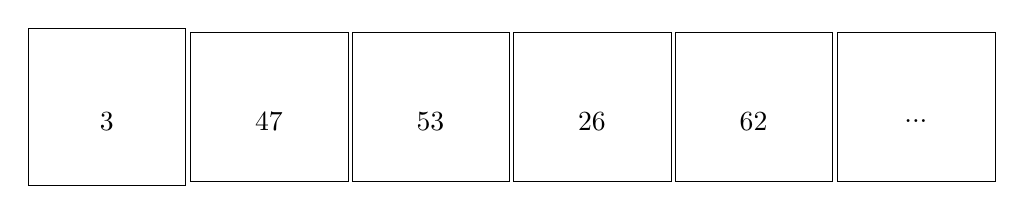
\begin{tikzpicture}
\pgftransformxscale{1.000000}
\pgftransformyscale{-1.000000}
\definecolor{dialinecolor}{rgb}{0.000000, 0.000000, 0.000000}
\pgfsetstrokecolor{dialinecolor}
\definecolor{dialinecolor}{rgb}{1.000000, 1.000000, 1.000000}
\pgfsetfillcolor{dialinecolor}
\definecolor{dialinecolor}{rgb}{1.000000, 1.000000, 1.000000}
\pgfsetfillcolor{dialinecolor}
\fill (46.050000\du,22.150000\du)--(46.050000\du,24.150000\du)--(48.050000\du,24.150000\du)--(48.050000\du,22.150000\du)--cycle;
\pgfsetlinewidth{0.200000\du}
\pgfsetdash{}{0pt}
\pgfsetdash{}{0pt}
\pgfsetmiterjoin
\definecolor{dialinecolor}{rgb}{0.000000, 0.000000, 0.000000}
\pgfsetstrokecolor{dialinecolor}
\draw (46.050000\du,22.150000\du)--(46.050000\du,24.150000\du)--(48.050000\du,24.150000\du)--(48.050000\du,22.150000\du)--cycle;
% setfont left to latex
\definecolor{dialinecolor}{rgb}{0.000000, 0.000000, 0.000000}
\pgfsetstrokecolor{dialinecolor}
\node at (47.050000\du,23.337500\du){3};
\definecolor{dialinecolor}{rgb}{1.000000, 1.000000, 1.000000}
\pgfsetfillcolor{dialinecolor}
\fill (48.110000\du,22.200000\du)--(48.110000\du,24.100000\du)--(50.110000\du,24.100000\du)--(50.110000\du,22.200000\du)--cycle;
\pgfsetlinewidth{0.100000\du}
\pgfsetdash{}{0pt}
\pgfsetdash{}{0pt}
\pgfsetmiterjoin
\definecolor{dialinecolor}{rgb}{0.000000, 0.000000, 0.000000}
\pgfsetstrokecolor{dialinecolor}
\draw (48.110000\du,22.200000\du)--(48.110000\du,24.100000\du)--(50.110000\du,24.100000\du)--(50.110000\du,22.200000\du)--cycle;
% setfont left to latex
\definecolor{dialinecolor}{rgb}{0.000000, 0.000000, 0.000000}
\pgfsetstrokecolor{dialinecolor}
\node at (49.110000\du,23.337500\du){47};
\definecolor{dialinecolor}{rgb}{1.000000, 1.000000, 1.000000}
\pgfsetfillcolor{dialinecolor}
\fill (50.161077\du,22.198863\du)--(50.161077\du,24.098863\du)--(52.161077\du,24.098863\du)--(52.161077\du,22.198863\du)--cycle;
\pgfsetlinewidth{0.100000\du}
\pgfsetdash{}{0pt}
\pgfsetdash{}{0pt}
\pgfsetmiterjoin
\definecolor{dialinecolor}{rgb}{0.000000, 0.000000, 0.000000}
\pgfsetstrokecolor{dialinecolor}
\draw (50.161077\du,22.198863\du)--(50.161077\du,24.098863\du)--(52.161077\du,24.098863\du)--(52.161077\du,22.198863\du)--cycle;
% setfont left to latex
\definecolor{dialinecolor}{rgb}{0.000000, 0.000000, 0.000000}
\pgfsetstrokecolor{dialinecolor}
\node at (51.161077\du,23.336363\du){53};
\definecolor{dialinecolor}{rgb}{1.000000, 1.000000, 1.000000}
\pgfsetfillcolor{dialinecolor}
\fill (52.212855\du,22.198863\du)--(52.212855\du,24.098863\du)--(54.212855\du,24.098863\du)--(54.212855\du,22.198863\du)--cycle;
\pgfsetlinewidth{0.100000\du}
\pgfsetdash{}{0pt}
\pgfsetdash{}{0pt}
\pgfsetmiterjoin
\definecolor{dialinecolor}{rgb}{0.000000, 0.000000, 0.000000}
\pgfsetstrokecolor{dialinecolor}
\draw (52.212855\du,22.198863\du)--(52.212855\du,24.098863\du)--(54.212855\du,24.098863\du)--(54.212855\du,22.198863\du)--cycle;
% setfont left to latex
\definecolor{dialinecolor}{rgb}{0.000000, 0.000000, 0.000000}
\pgfsetstrokecolor{dialinecolor}
\node at (53.212855\du,23.336363\du){26};
\definecolor{dialinecolor}{rgb}{1.000000, 1.000000, 1.000000}
\pgfsetfillcolor{dialinecolor}
\fill (54.264633\du,22.198863\du)--(54.264633\du,24.098863\du)--(56.264633\du,24.098863\du)--(56.264633\du,22.198863\du)--cycle;
\pgfsetlinewidth{0.100000\du}
\pgfsetdash{}{0pt}
\pgfsetdash{}{0pt}
\pgfsetmiterjoin
\definecolor{dialinecolor}{rgb}{0.000000, 0.000000, 0.000000}
\pgfsetstrokecolor{dialinecolor}
\draw (54.264633\du,22.198863\du)--(54.264633\du,24.098863\du)--(56.264633\du,24.098863\du)--(56.264633\du,22.198863\du)--cycle;
% setfont left to latex
\definecolor{dialinecolor}{rgb}{0.000000, 0.000000, 0.000000}
\pgfsetstrokecolor{dialinecolor}
\node at (55.264633\du,23.336363\du){62};
\definecolor{dialinecolor}{rgb}{1.000000, 1.000000, 1.000000}
\pgfsetfillcolor{dialinecolor}
\fill (56.326923\du,22.198863\du)--(56.326923\du,24.098863\du)--(58.326923\du,24.098863\du)--(58.326923\du,22.198863\du)--cycle;
\pgfsetlinewidth{0.100000\du}
\pgfsetdash{}{0pt}
\pgfsetdash{}{0pt}
\pgfsetmiterjoin
\definecolor{dialinecolor}{rgb}{0.000000, 0.000000, 0.000000}
\pgfsetstrokecolor{dialinecolor}
\draw (56.326923\du,22.198863\du)--(56.326923\du,24.098863\du)--(58.326923\du,24.098863\du)--(58.326923\du,22.198863\du)--cycle;
% setfont left to latex
\definecolor{dialinecolor}{rgb}{0.000000, 0.000000, 0.000000}
\pgfsetstrokecolor{dialinecolor}
\node at (57.326923\du,23.336363\du){...};
\end{tikzpicture}

  \caption{Beispielhafte vierte Dimension der Datenstruktur}
  \label{fig:datenstruktur_eintraege}
\end{figure}

\begin{minipage}{\linewidth}
\begin{lstlisting}[caption=Iteration über benachbarte Partikel, label=lst:grid_for]
int4 gridPos = convert_int4((BUFFER_SIZE_SIDE - 1) * (body_Pos[id] + (float4)1) / 2);
for (int l = max(gridPos.x - OFFSET, 0); l <= min(gridPos.x + OFFSET, BUFFER_SIZE_SIDE - 1) ; l++) {
	for (int j = max(gridPos.y - OFFSET, 0); j <= min(gridPos.y + OFFSET, BUFFER_SIZE_SIDE - 1) ; j++) {
		for (int k = max(gridPos.z - OFFSET, 0); k <= min(gridPos.z + OFFSET, BUFFER_SIZE_SIDE - 1) ; k++) {
			int cnt_ind = BUFFER_SIZE_DEPTH * (l + BUFFER_SIZE_SIDE * j + BUFFER_SIZE_SIDE * BUFFER_SIZE_SIDE * k);
			uint cnt = data[cnt_ind];			
			for (int o = 1; o <= cnt; o++) {
				int i = data[cnt_ind + o];
				...
			}
		}
	}
}
\end{lstlisting}
\end{minipage}

Mithilfe dieses Arrays lässt sich nun, zu sehen in Code~\ref{lst:grid_for}, über alle benachbarten Partikel iterieren. Die Konstante \texttt{BUFFER\_SIZE\_SIDE} gibt dabei die Anzahl an Zellen für jede der ersten drei Dimensionen an und \texttt{BUFFER\_SIZE\_DEPTH} der reservierte Platz für Partikel innerhalb einer Zelle, also die vierte Dimension, wobei mithilfe von \texttt{OFFSET} der gewünschte Radius um die betrachtete Zelle festgelegt wird.


Alle diese Konstanten können unabhängig von der Partikelzahl gewählt werden, mit Ausnahme von \texttt{BUFFER\_SIZE\_DEPTH}. Ist diese Konstante zu gering, könnte der verfügbare Speicherplatz bei zu vielen Partikeln innerhalb einer Zelle überlaufen. Sollte dieser Fall eintreten, werden alle nachfolgenden Partikel dieser Zelle nicht gespeichert, und werden bei den folgenden Nachbarschaftsberechnungen dementsprechend solange nicht berücksichtigt, bis sie wieder einen Platz finden.\\
Als \textit{guter} Wert für \texttt{BUFFER\_SIZE\_DEPTH} hat sich $\sqrt(n)$ bewiesen, wobei auch zu geringe Werte, die einen Überlauf induzieren, vor allem bei einer hohen Partikelanzahl erst spät zu Veränderungen in der Simulation führen, da nur einzelne Partikel davon betroffen sind.\\
Wenn man nun davon ausgeht, dass $\sqrt(n)$ ein guter Wert für \texttt{BUFFER\_SIZE\_DEPTH} sei, dann hat die Schleife, die über die benachbarten Partikel iteriert, eine Laufzeit von $\mathcal O(\sqrt(n))$ im worst-case. Dadurch verbessert sich die asymptotische Laufzeit des gesamten Algorithmus' auf $\mathcal O(n \cdot \sqrt(n))$.
\subsubsection{Speicherung der Partikelindices in einer dreidimensionalen Textur}
Dieser Ansatz wurde nur diskutiert, da die vorhergehende Herangehensweise bereits zufriedenstellende Ergebnisse lieferte.\\
Die Grundidee hierbei ist, für die Partikelindices statt einem vierdimensionalen Array eine dreidimensionale Textur zu verwenden, wobei die eigentlichen Indices - vorher abgelegt in der vierten Dimension - nun in den vier Farbkanälen der Textur codiert werden müssen. Da diese Kanäle nur begrenzten Platz zur Verfügung stellen, müsste die Textur tendenziell höher aufgelöst sein als das Grid beim vorigen Ansatz, um einen Überlauf zu vermeiden. Dadurch würde zweifellos ein erhöhter Aufwand entstehen, der aber, so die Idee, dennoch zu einer schnelleren Laufzeit führen könnte aufgrund des internen Cachings durch die Grafikkarte. Da sich die Partikel allerdings stets bewegen, müssten die gespeicherten Indices in jedem Zeitschritt modifiziert werden, was effizientem Caching entgegenwirkt. Die Frage, ob dieser Ansatz effizienter als der vorhergehende ist, lässt sich also auf die Frage, ob das Caching bei erhöhtem Lesezugriff und gleichbleibendem Schreibzugriff zu einer schnelleren Laufzeit führt als bei herkömmlichen globalen Speicher, abbilden. Da die Antwort unklar und somit der Gewinn durch diesen Ansatz in Frage gestellt wurde, wurde er verworfen.
\subsubsection{Zufallsbasierte Selektion einer Referenzmenge}
Bei diesem Ansatz sollte die Laufzeit verringert werden, indem die zur Kräfteberechnung herangezogenen Partikel einer zufällig ausgewählten und echten Teilmenge aller Partikel entstammen. Bei einer entsprechend gewählten Größe dieser Teilmenge konnte diese außerdem im lokalen Speicher abgelegt werden, um die Laufzeit weiter zu reduzieren.\\
Es hat sich allerdings gezeigt, dass die Genauigkeit der Simulation durch diesen Ansatz signifikant verschlechtert wurde, sodass er - trotz überragend schneller Laufzeit - wieder verworfen wurde.
\subsection{OpenCL und Parallelisierung}
Wie bei einem herkömmlichen n-Body-System können auch bei dieser Simulation die Zustandsberechnungen der einzelnen Partikel unabhängig von den jeweils anderen durchgeführt werden. Da die Berechnungen allerdings von den Zuständen der anderen Partikel abhängen, welche wiederum ebenfalls einen neuen Zustand errechnen, muss mithilfe von Synchronisation sichergestellt werden, dass keine ungewünschten Seiteneffekte durch teilweise modifizierte Daten entstehen.\\
Da sich die Partikel aufgrund ihrer stetigen Bewegung und damit wechselnden Abhängigkeiten nicht sinnvoll mithilfe von Work Groups aufteilen ließen, wurden die Teilschritte der Berechnung in einzelne Kernel ausgelagert, die auf diese Weise global synchronisiert werden können.\\
Der grundlegende Ablauf ist hierbei in Abbildung~\ref{fig:simulation_kernelablauf} zu erkennen. Für die Berechnung eines neuen Geschwindigkeitsvektors \texttt{V} werden sowohl Druck $\rho$  als auch Dichte \texttt{P} des Partikels benötigt, welche wiederum voneinander und von anderen Partikeln abhängen. Aus diesem Grunde wird zuerst $\rho$ für alle Partikel berechnet, damit, nach einem Synchronisationspunkt, \texttt{P} mithilfe von $\rho$ berechnet werden kann. \\
Der Synchronisationspunkt nach der Berechnung der neuen Geschwindigkeit hat keine technische Grundlage, da die neue Position des Partikels nur von den eigenen Attributen ahängig ist, wurde aber zwecks Profiling eingeführt.
\begin{figure}[h]
  \centering
    % Graphic for TeX using PGF
% Title: D:\workspace\uos_pa_sph\doku\images\simulation_kernelablauf.dia
% Creator: Dia v0.97.2
% CreationDate: Fri Sep 13 15:07:09 2013
% For: Nikki
% \usepackage{tikz}
% The following commands are not supported in PSTricks at present
% We define them conditionally, so when they are implemented,
% this pgf file will use them.
\ifx\du\undefined
  \newlength{\du}
\fi
\setlength{\du}{15\unitlength}
\begin{tikzpicture}
\pgftransformxscale{0.600000}
\pgftransformyscale{-0.600000}
\definecolor{dialinecolor}{rgb}{0.000000, 0.000000, 0.000000}
\pgfsetstrokecolor{dialinecolor}
\definecolor{dialinecolor}{rgb}{1.000000, 1.000000, 1.000000}
\pgfsetfillcolor{dialinecolor}
\definecolor{dialinecolor}{rgb}{1.000000, 1.000000, 1.000000}
\pgfsetfillcolor{dialinecolor}
\fill (18.462586\du,22.197519\du)--(18.462586\du,31.589660\du)--(41.526766\du,31.589660\du)--(41.526766\du,22.197519\du)--cycle;
\pgfsetlinewidth{0.100000\du}
\pgfsetdash{}{0pt}
\pgfsetdash{}{0pt}
\pgfsetmiterjoin
\definecolor{dialinecolor}{rgb}{0.000000, 0.000000, 0.000000}
\pgfsetstrokecolor{dialinecolor}
\draw (18.462586\du,22.197519\du)--(18.462586\du,31.589660\du)--(41.526766\du,31.589660\du)--(41.526766\du,22.197519\du)--cycle;
% setfont left to latex
\definecolor{dialinecolor}{rgb}{0.000000, 0.000000, 0.000000}
\pgfsetstrokecolor{dialinecolor}
\node at (29.994676\du,27.133589\du){};
\pgfsetlinewidth{0.100000\du}
\pgfsetdash{}{0pt}
\pgfsetdash{}{0pt}
\pgfsetbuttcap
{
\definecolor{dialinecolor}{rgb}{0.000000, 0.000000, 0.000000}
\pgfsetfillcolor{dialinecolor}
% was here!!!
\pgfsetarrowsend{latex}
\definecolor{dialinecolor}{rgb}{0.000000, 0.000000, 0.000000}
\pgfsetstrokecolor{dialinecolor}
\draw (47.125778\du,24.028174\du)--(47.100000\du,26.300000\du);
}
\pgfsetlinewidth{0.100000\du}
\pgfsetdash{}{0pt}
\pgfsetdash{}{0pt}
\pgfsetbuttcap
{
\definecolor{dialinecolor}{rgb}{0.000000, 0.000000, 0.000000}
\pgfsetfillcolor{dialinecolor}
% was here!!!
\pgfsetarrowsend{latex}
\definecolor{dialinecolor}{rgb}{0.000000, 0.000000, 0.000000}
\pgfsetstrokecolor{dialinecolor}
\draw (51.043113\du,24.057252\du)--(47.100000\du,26.300000\du);
}
\pgfsetlinewidth{0.100000\du}
\pgfsetdash{}{0pt}
\pgfsetdash{}{0pt}
\pgfsetbuttcap
{
\definecolor{dialinecolor}{rgb}{0.000000, 0.000000, 0.000000}
\pgfsetfillcolor{dialinecolor}
% was here!!!
\pgfsetarrowsend{latex}
\definecolor{dialinecolor}{rgb}{0.000000, 0.000000, 0.000000}
\pgfsetstrokecolor{dialinecolor}
\draw (60.013113\du,24.057252\du)--(47.100000\du,26.300000\du);
}
\pgfsetlinewidth{0.100000\du}
\pgfsetdash{}{0pt}
\pgfsetdash{}{0pt}
\pgfsetbuttcap
{
\definecolor{dialinecolor}{rgb}{0.000000, 0.000000, 0.000000}
\pgfsetfillcolor{dialinecolor}
% was here!!!
\pgfsetarrowsend{latex}
\definecolor{dialinecolor}{rgb}{0.000000, 0.000000, 0.000000}
\pgfsetstrokecolor{dialinecolor}
\draw (51.043113\du,24.057252\du)--(51.000000\du,26.250000\du);
}
\pgfsetlinewidth{0.100000\du}
\pgfsetdash{}{0pt}
\pgfsetdash{}{0pt}
\pgfsetbuttcap
{
\definecolor{dialinecolor}{rgb}{0.000000, 0.000000, 0.000000}
\pgfsetfillcolor{dialinecolor}
% was here!!!
\pgfsetarrowsend{latex}
\definecolor{dialinecolor}{rgb}{0.000000, 0.000000, 0.000000}
\pgfsetstrokecolor{dialinecolor}
\draw (55.003113\du,24.107252\du)--(51.000000\du,26.250000\du);
}
\pgfsetlinewidth{0.100000\du}
\pgfsetdash{}{0pt}
\pgfsetdash{}{0pt}
\pgfsetbuttcap
{
\definecolor{dialinecolor}{rgb}{0.000000, 0.000000, 0.000000}
\pgfsetfillcolor{dialinecolor}
% was here!!!
\pgfsetarrowsend{latex}
\definecolor{dialinecolor}{rgb}{0.000000, 0.000000, 0.000000}
\pgfsetstrokecolor{dialinecolor}
\draw (55.003113\du,24.107252\du)--(55.000000\du,26.300000\du);
}
\pgfsetlinewidth{0.100000\du}
\pgfsetdash{}{0pt}
\pgfsetdash{}{0pt}
\pgfsetbuttcap
{
\definecolor{dialinecolor}{rgb}{0.000000, 0.000000, 0.000000}
\pgfsetfillcolor{dialinecolor}
% was here!!!
\pgfsetarrowsend{latex}
\definecolor{dialinecolor}{rgb}{0.000000, 0.000000, 0.000000}
\pgfsetstrokecolor{dialinecolor}
\draw (47.125778\du,24.028174\du)--(55.000000\du,26.350000\du);
}
\pgfsetlinewidth{0.100000\du}
\pgfsetdash{}{0pt}
\pgfsetdash{}{0pt}
\pgfsetbuttcap
{
\definecolor{dialinecolor}{rgb}{0.000000, 0.000000, 0.000000}
\pgfsetfillcolor{dialinecolor}
% was here!!!
\pgfsetarrowsend{latex}
\definecolor{dialinecolor}{rgb}{0.000000, 0.000000, 0.000000}
\pgfsetstrokecolor{dialinecolor}
\draw (60.013113\du,24.057252\du)--(59.950000\du,26.300000\du);
}
\pgfsetlinewidth{0.100000\du}
\pgfsetdash{}{0pt}
\pgfsetdash{}{0pt}
\pgfsetbuttcap
{
\definecolor{dialinecolor}{rgb}{0.000000, 0.000000, 0.000000}
\pgfsetfillcolor{dialinecolor}
% was here!!!
\pgfsetarrowsend{latex}
\definecolor{dialinecolor}{rgb}{0.000000, 0.000000, 0.000000}
\pgfsetstrokecolor{dialinecolor}
\draw (51.043113\du,24.057252\du)--(59.950000\du,26.350000\du);
}
\definecolor{dialinecolor}{rgb}{1.000000, 1.000000, 1.000000}
\pgfsetfillcolor{dialinecolor}
\pgfpathellipse{\pgfpoint{47.521160\du}{31.381493\du}}{\pgfpoint{1.419866\du}{0\du}}{\pgfpoint{0\du}{1.403171\du}}
\pgfusepath{fill}
\pgfsetlinewidth{0.100000\du}
\pgfsetdash{}{0pt}
\pgfsetdash{}{0pt}
\pgfsetmiterjoin
\definecolor{dialinecolor}{rgb}{0.000000, 0.000000, 0.000000}
\pgfsetstrokecolor{dialinecolor}
\pgfpathellipse{\pgfpoint{47.521160\du}{31.381493\du}}{\pgfpoint{1.419866\du}{0\du}}{\pgfpoint{0\du}{1.403171\du}}
\pgfusepath{stroke}
% setfont left to latex
\definecolor{dialinecolor}{rgb}{0.000000, 0.000000, 0.000000}
\pgfsetstrokecolor{dialinecolor}
\node at (47.521160\du,31.513993\du){Rho1};
\definecolor{dialinecolor}{rgb}{1.000000, 1.000000, 1.000000}
\pgfsetfillcolor{dialinecolor}
\pgfpathellipse{\pgfpoint{51.029866\du}{31.453171\du}}{\pgfpoint{1.419866\du}{0\du}}{\pgfpoint{0\du}{1.403171\du}}
\pgfusepath{fill}
\pgfsetlinewidth{0.100000\du}
\pgfsetdash{}{0pt}
\pgfsetdash{}{0pt}
\pgfsetmiterjoin
\definecolor{dialinecolor}{rgb}{0.000000, 0.000000, 0.000000}
\pgfsetstrokecolor{dialinecolor}
\pgfpathellipse{\pgfpoint{51.029866\du}{31.453171\du}}{\pgfpoint{1.419866\du}{0\du}}{\pgfpoint{0\du}{1.403171\du}}
\pgfusepath{stroke}
% setfont left to latex
\definecolor{dialinecolor}{rgb}{0.000000, 0.000000, 0.000000}
\pgfsetstrokecolor{dialinecolor}
\node at (51.029866\du,31.585671\du){Rho2};
\definecolor{dialinecolor}{rgb}{1.000000, 1.000000, 1.000000}
\pgfsetfillcolor{dialinecolor}
\pgfpathellipse{\pgfpoint{54.939866\du}{31.453171\du}}{\pgfpoint{1.419866\du}{0\du}}{\pgfpoint{0\du}{1.403171\du}}
\pgfusepath{fill}
\pgfsetlinewidth{0.100000\du}
\pgfsetdash{}{0pt}
\pgfsetdash{}{0pt}
\pgfsetmiterjoin
\definecolor{dialinecolor}{rgb}{0.000000, 0.000000, 0.000000}
\pgfsetstrokecolor{dialinecolor}
\pgfpathellipse{\pgfpoint{54.939866\du}{31.453171\du}}{\pgfpoint{1.419866\du}{0\du}}{\pgfpoint{0\du}{1.403171\du}}
\pgfusepath{stroke}
% setfont left to latex
\definecolor{dialinecolor}{rgb}{0.000000, 0.000000, 0.000000}
\pgfsetstrokecolor{dialinecolor}
\node at (54.939866\du,31.585671\du){Rho3};
\definecolor{dialinecolor}{rgb}{1.000000, 1.000000, 1.000000}
\pgfsetfillcolor{dialinecolor}
\pgfpathellipse{\pgfpoint{59.949866\du}{31.453171\du}}{\pgfpoint{1.419866\du}{0\du}}{\pgfpoint{0\du}{1.403171\du}}
\pgfusepath{fill}
\pgfsetlinewidth{0.100000\du}
\pgfsetdash{}{0pt}
\pgfsetdash{}{0pt}
\pgfsetmiterjoin
\definecolor{dialinecolor}{rgb}{0.000000, 0.000000, 0.000000}
\pgfsetstrokecolor{dialinecolor}
\pgfpathellipse{\pgfpoint{59.949866\du}{31.453171\du}}{\pgfpoint{1.419866\du}{0\du}}{\pgfpoint{0\du}{1.403171\du}}
\pgfusepath{stroke}
% setfont left to latex
\definecolor{dialinecolor}{rgb}{0.000000, 0.000000, 0.000000}
\pgfsetstrokecolor{dialinecolor}
\node at (59.949866\du,31.585671\du){Rhon};
\pgfsetlinewidth{0.100000\du}
\pgfsetdash{}{0pt}
\pgfsetdash{}{0pt}
\pgfsetbuttcap
{
\definecolor{dialinecolor}{rgb}{0.000000, 0.000000, 0.000000}
\pgfsetfillcolor{dialinecolor}
% was here!!!
\pgfsetarrowsend{latex}
\definecolor{dialinecolor}{rgb}{0.000000, 0.000000, 0.000000}
\pgfsetstrokecolor{dialinecolor}
\draw (47.500000\du,28.400000\du)--(47.521160\du,29.978322\du);
}
\pgfsetlinewidth{0.100000\du}
\pgfsetdash{}{0pt}
\pgfsetdash{}{0pt}
\pgfsetbuttcap
{
\definecolor{dialinecolor}{rgb}{0.000000, 0.000000, 0.000000}
\pgfsetfillcolor{dialinecolor}
% was here!!!
\pgfsetarrowsend{latex}
\definecolor{dialinecolor}{rgb}{0.000000, 0.000000, 0.000000}
\pgfsetstrokecolor{dialinecolor}
\draw (51.000000\du,28.350000\du)--(51.029866\du,30.050000\du);
}
\pgfsetlinewidth{0.100000\du}
\pgfsetdash{}{0pt}
\pgfsetdash{}{0pt}
\pgfsetbuttcap
{
\definecolor{dialinecolor}{rgb}{0.000000, 0.000000, 0.000000}
\pgfsetfillcolor{dialinecolor}
% was here!!!
\pgfsetarrowsend{latex}
\definecolor{dialinecolor}{rgb}{0.000000, 0.000000, 0.000000}
\pgfsetstrokecolor{dialinecolor}
\draw (55.000000\du,28.400000\du)--(54.939866\du,30.050000\du);
}
\pgfsetlinewidth{0.100000\du}
\pgfsetdash{}{0pt}
\pgfsetdash{}{0pt}
\pgfsetbuttcap
{
\definecolor{dialinecolor}{rgb}{0.000000, 0.000000, 0.000000}
\pgfsetfillcolor{dialinecolor}
% was here!!!
\pgfsetarrowsend{latex}
\definecolor{dialinecolor}{rgb}{0.000000, 0.000000, 0.000000}
\pgfsetstrokecolor{dialinecolor}
\draw (60.050000\du,28.350000\du)--(59.949866\du,30.050000\du);
}
\definecolor{dialinecolor}{rgb}{1.000000, 1.000000, 1.000000}
\pgfsetfillcolor{dialinecolor}
\fill (43.980402\du,26.300000\du)--(43.980402\du,28.500000\du)--(63.009714\du,28.500000\du)--(63.009714\du,26.300000\du)--cycle;
\pgfsetlinewidth{0.100000\du}
\pgfsetdash{}{0pt}
\pgfsetdash{}{0pt}
\pgfsetmiterjoin
\definecolor{dialinecolor}{rgb}{0.000000, 0.000000, 0.000000}
\pgfsetstrokecolor{dialinecolor}
\draw (43.980402\du,26.300000\du)--(43.980402\du,28.500000\du)--(63.009714\du,28.500000\du)--(63.009714\du,26.300000\du)--cycle;
% setfont left to latex
\definecolor{dialinecolor}{rgb}{0.000000, 0.000000, 0.000000}
\pgfsetstrokecolor{dialinecolor}
\node at (53.495058\du,27.640000\du){Berechne Dichte (Rho)};
\pgfsetlinewidth{0.100000\du}
\pgfsetdash{}{0pt}
\pgfsetdash{}{0pt}
\pgfsetbuttcap
{
\definecolor{dialinecolor}{rgb}{0.000000, 0.000000, 0.000000}
\pgfsetfillcolor{dialinecolor}
% was here!!!
\pgfsetarrowsend{latex}
\definecolor{dialinecolor}{rgb}{0.000000, 0.000000, 0.000000}
\pgfsetstrokecolor{dialinecolor}
\draw (47.235778\du,32.712100\du)--(47.210000\du,34.983925\du);
}
\pgfsetlinewidth{0.100000\du}
\pgfsetdash{}{0pt}
\pgfsetdash{}{0pt}
\pgfsetbuttcap
{
\definecolor{dialinecolor}{rgb}{0.000000, 0.000000, 0.000000}
\pgfsetfillcolor{dialinecolor}
% was here!!!
\pgfsetarrowsend{latex}
\definecolor{dialinecolor}{rgb}{0.000000, 0.000000, 0.000000}
\pgfsetstrokecolor{dialinecolor}
\draw (51.153113\du,32.741178\du)--(47.210000\du,34.983925\du);
}
\pgfsetlinewidth{0.100000\du}
\pgfsetdash{}{0pt}
\pgfsetdash{}{0pt}
\pgfsetbuttcap
{
\definecolor{dialinecolor}{rgb}{0.000000, 0.000000, 0.000000}
\pgfsetfillcolor{dialinecolor}
% was here!!!
\pgfsetarrowsend{latex}
\definecolor{dialinecolor}{rgb}{0.000000, 0.000000, 0.000000}
\pgfsetstrokecolor{dialinecolor}
\draw (60.123113\du,32.741178\du)--(47.210000\du,34.983925\du);
}
\pgfsetlinewidth{0.100000\du}
\pgfsetdash{}{0pt}
\pgfsetdash{}{0pt}
\pgfsetbuttcap
{
\definecolor{dialinecolor}{rgb}{0.000000, 0.000000, 0.000000}
\pgfsetfillcolor{dialinecolor}
% was here!!!
\pgfsetarrowsend{latex}
\definecolor{dialinecolor}{rgb}{0.000000, 0.000000, 0.000000}
\pgfsetstrokecolor{dialinecolor}
\draw (51.153113\du,32.741178\du)--(51.110000\du,34.933925\du);
}
\pgfsetlinewidth{0.100000\du}
\pgfsetdash{}{0pt}
\pgfsetdash{}{0pt}
\pgfsetbuttcap
{
\definecolor{dialinecolor}{rgb}{0.000000, 0.000000, 0.000000}
\pgfsetfillcolor{dialinecolor}
% was here!!!
\pgfsetarrowsend{latex}
\definecolor{dialinecolor}{rgb}{0.000000, 0.000000, 0.000000}
\pgfsetstrokecolor{dialinecolor}
\draw (55.113113\du,32.791178\du)--(51.110000\du,34.933925\du);
}
\pgfsetlinewidth{0.100000\du}
\pgfsetdash{}{0pt}
\pgfsetdash{}{0pt}
\pgfsetbuttcap
{
\definecolor{dialinecolor}{rgb}{0.000000, 0.000000, 0.000000}
\pgfsetfillcolor{dialinecolor}
% was here!!!
\pgfsetarrowsend{latex}
\definecolor{dialinecolor}{rgb}{0.000000, 0.000000, 0.000000}
\pgfsetstrokecolor{dialinecolor}
\draw (55.113113\du,32.791178\du)--(55.110000\du,34.983925\du);
}
\pgfsetlinewidth{0.100000\du}
\pgfsetdash{}{0pt}
\pgfsetdash{}{0pt}
\pgfsetbuttcap
{
\definecolor{dialinecolor}{rgb}{0.000000, 0.000000, 0.000000}
\pgfsetfillcolor{dialinecolor}
% was here!!!
\pgfsetarrowsend{latex}
\definecolor{dialinecolor}{rgb}{0.000000, 0.000000, 0.000000}
\pgfsetstrokecolor{dialinecolor}
\draw (47.235778\du,32.712100\du)--(55.110000\du,35.033925\du);
}
\pgfsetlinewidth{0.100000\du}
\pgfsetdash{}{0pt}
\pgfsetdash{}{0pt}
\pgfsetbuttcap
{
\definecolor{dialinecolor}{rgb}{0.000000, 0.000000, 0.000000}
\pgfsetfillcolor{dialinecolor}
% was here!!!
\pgfsetarrowsend{latex}
\definecolor{dialinecolor}{rgb}{0.000000, 0.000000, 0.000000}
\pgfsetstrokecolor{dialinecolor}
\draw (60.123113\du,32.741178\du)--(60.060000\du,34.983925\du);
}
\pgfsetlinewidth{0.100000\du}
\pgfsetdash{}{0pt}
\pgfsetdash{}{0pt}
\pgfsetbuttcap
{
\definecolor{dialinecolor}{rgb}{0.000000, 0.000000, 0.000000}
\pgfsetfillcolor{dialinecolor}
% was here!!!
\pgfsetarrowsend{latex}
\definecolor{dialinecolor}{rgb}{0.000000, 0.000000, 0.000000}
\pgfsetstrokecolor{dialinecolor}
\draw (51.153113\du,32.741178\du)--(60.060000\du,35.033925\du);
}
\definecolor{dialinecolor}{rgb}{1.000000, 1.000000, 1.000000}
\pgfsetfillcolor{dialinecolor}
\fill (43.980402\du,34.933925\du)--(43.980402\du,37.200000\du)--(63.009714\du,37.200000\du)--(63.009714\du,34.933925\du)--cycle;
\pgfsetlinewidth{0.100000\du}
\pgfsetdash{}{0pt}
\pgfsetdash{}{0pt}
\pgfsetmiterjoin
\definecolor{dialinecolor}{rgb}{0.000000, 0.000000, 0.000000}
\pgfsetstrokecolor{dialinecolor}
\draw (43.980402\du,34.933925\du)--(43.980402\du,37.200000\du)--(63.009714\du,37.200000\du)--(63.009714\du,34.933925\du)--cycle;
% setfont left to latex
\definecolor{dialinecolor}{rgb}{0.000000, 0.000000, 0.000000}
\pgfsetstrokecolor{dialinecolor}
\node at (53.495058\du,36.306963\du){Berechne Druck (P)};
\pgfsetlinewidth{0.300000\du}
\pgfsetdash{{1.000000\du}{1.000000\du}}{0\du}
\pgfsetdash{{1.000000\du}{1.000000\du}}{0\du}
\pgfsetbuttcap
{
\definecolor{dialinecolor}{rgb}{0.000000, 0.000000, 0.000000}
\pgfsetfillcolor{dialinecolor}
% was here!!!
\definecolor{dialinecolor}{rgb}{0.000000, 0.000000, 0.000000}
\pgfsetstrokecolor{dialinecolor}
\draw (44.300000\du,33.800000\du)--(63.250000\du,33.750000\du);
}
\definecolor{dialinecolor}{rgb}{1.000000, 1.000000, 1.000000}
\pgfsetfillcolor{dialinecolor}
\pgfpathellipse{\pgfpoint{47.579866\du}{40.184346\du}}{\pgfpoint{1.419866\du}{0\du}}{\pgfpoint{0\du}{1.403171\du}}
\pgfusepath{fill}
\pgfsetlinewidth{0.100000\du}
\pgfsetdash{}{0pt}
\pgfsetdash{}{0pt}
\pgfsetmiterjoin
\definecolor{dialinecolor}{rgb}{0.000000, 0.000000, 0.000000}
\pgfsetstrokecolor{dialinecolor}
\pgfpathellipse{\pgfpoint{47.579866\du}{40.184346\du}}{\pgfpoint{1.419866\du}{0\du}}{\pgfpoint{0\du}{1.403171\du}}
\pgfusepath{stroke}
% setfont left to latex
\definecolor{dialinecolor}{rgb}{0.000000, 0.000000, 0.000000}
\pgfsetstrokecolor{dialinecolor}
\node at (47.579866\du,40.316846\du){P1};
\definecolor{dialinecolor}{rgb}{1.000000, 1.000000, 1.000000}
\pgfsetfillcolor{dialinecolor}
\pgfpathellipse{\pgfpoint{51.088572\du}{40.256025\du}}{\pgfpoint{1.419866\du}{0\du}}{\pgfpoint{0\du}{1.403171\du}}
\pgfusepath{fill}
\pgfsetlinewidth{0.100000\du}
\pgfsetdash{}{0pt}
\pgfsetdash{}{0pt}
\pgfsetmiterjoin
\definecolor{dialinecolor}{rgb}{0.000000, 0.000000, 0.000000}
\pgfsetstrokecolor{dialinecolor}
\pgfpathellipse{\pgfpoint{51.088572\du}{40.256025\du}}{\pgfpoint{1.419866\du}{0\du}}{\pgfpoint{0\du}{1.403171\du}}
\pgfusepath{stroke}
% setfont left to latex
\definecolor{dialinecolor}{rgb}{0.000000, 0.000000, 0.000000}
\pgfsetstrokecolor{dialinecolor}
\node at (51.088572\du,40.388525\du){P2};
\definecolor{dialinecolor}{rgb}{1.000000, 1.000000, 1.000000}
\pgfsetfillcolor{dialinecolor}
\pgfpathellipse{\pgfpoint{54.998572\du}{40.256025\du}}{\pgfpoint{1.419866\du}{0\du}}{\pgfpoint{0\du}{1.403171\du}}
\pgfusepath{fill}
\pgfsetlinewidth{0.100000\du}
\pgfsetdash{}{0pt}
\pgfsetdash{}{0pt}
\pgfsetmiterjoin
\definecolor{dialinecolor}{rgb}{0.000000, 0.000000, 0.000000}
\pgfsetstrokecolor{dialinecolor}
\pgfpathellipse{\pgfpoint{54.998572\du}{40.256025\du}}{\pgfpoint{1.419866\du}{0\du}}{\pgfpoint{0\du}{1.403171\du}}
\pgfusepath{stroke}
% setfont left to latex
\definecolor{dialinecolor}{rgb}{0.000000, 0.000000, 0.000000}
\pgfsetstrokecolor{dialinecolor}
\node at (54.998572\du,40.388525\du){P3};
\definecolor{dialinecolor}{rgb}{1.000000, 1.000000, 1.000000}
\pgfsetfillcolor{dialinecolor}
\pgfpathellipse{\pgfpoint{60.008572\du}{40.256025\du}}{\pgfpoint{1.419866\du}{0\du}}{\pgfpoint{0\du}{1.403171\du}}
\pgfusepath{fill}
\pgfsetlinewidth{0.100000\du}
\pgfsetdash{}{0pt}
\pgfsetdash{}{0pt}
\pgfsetmiterjoin
\definecolor{dialinecolor}{rgb}{0.000000, 0.000000, 0.000000}
\pgfsetstrokecolor{dialinecolor}
\pgfpathellipse{\pgfpoint{60.008572\du}{40.256025\du}}{\pgfpoint{1.419866\du}{0\du}}{\pgfpoint{0\du}{1.403171\du}}
\pgfusepath{stroke}
% setfont left to latex
\definecolor{dialinecolor}{rgb}{0.000000, 0.000000, 0.000000}
\pgfsetstrokecolor{dialinecolor}
\node at (60.008572\du,40.388525\du){Pn};
\pgfsetlinewidth{0.100000\du}
\pgfsetdash{}{0pt}
\pgfsetdash{}{0pt}
\pgfsetbuttcap
{
\definecolor{dialinecolor}{rgb}{0.000000, 0.000000, 0.000000}
\pgfsetfillcolor{dialinecolor}
% was here!!!
\pgfsetarrowsend{latex}
\definecolor{dialinecolor}{rgb}{0.000000, 0.000000, 0.000000}
\pgfsetstrokecolor{dialinecolor}
\draw (47.558706\du,37.202854\du)--(47.579866\du,38.781175\du);
}
\pgfsetlinewidth{0.100000\du}
\pgfsetdash{}{0pt}
\pgfsetdash{}{0pt}
\pgfsetbuttcap
{
\definecolor{dialinecolor}{rgb}{0.000000, 0.000000, 0.000000}
\pgfsetfillcolor{dialinecolor}
% was here!!!
\pgfsetarrowsend{latex}
\definecolor{dialinecolor}{rgb}{0.000000, 0.000000, 0.000000}
\pgfsetstrokecolor{dialinecolor}
\draw (51.058706\du,37.152854\du)--(51.088572\du,38.852854\du);
}
\pgfsetlinewidth{0.100000\du}
\pgfsetdash{}{0pt}
\pgfsetdash{}{0pt}
\pgfsetbuttcap
{
\definecolor{dialinecolor}{rgb}{0.000000, 0.000000, 0.000000}
\pgfsetfillcolor{dialinecolor}
% was here!!!
\pgfsetarrowsend{latex}
\definecolor{dialinecolor}{rgb}{0.000000, 0.000000, 0.000000}
\pgfsetstrokecolor{dialinecolor}
\draw (55.058706\du,37.202854\du)--(54.998572\du,38.852854\du);
}
\pgfsetlinewidth{0.100000\du}
\pgfsetdash{}{0pt}
\pgfsetdash{}{0pt}
\pgfsetbuttcap
{
\definecolor{dialinecolor}{rgb}{0.000000, 0.000000, 0.000000}
\pgfsetfillcolor{dialinecolor}
% was here!!!
\pgfsetarrowsend{latex}
\definecolor{dialinecolor}{rgb}{0.000000, 0.000000, 0.000000}
\pgfsetstrokecolor{dialinecolor}
\draw (60.108706\du,37.152854\du)--(60.008572\du,38.852854\du);
}
\pgfsetlinewidth{0.100000\du}
\pgfsetdash{}{0pt}
\pgfsetdash{}{0pt}
\pgfsetbuttcap
{
\definecolor{dialinecolor}{rgb}{0.000000, 0.000000, 0.000000}
\pgfsetfillcolor{dialinecolor}
% was here!!!
\pgfsetarrowsend{latex}
\definecolor{dialinecolor}{rgb}{0.000000, 0.000000, 0.000000}
\pgfsetstrokecolor{dialinecolor}
\draw (46.986507\du,46.199532\du)--(47.117334\du,48.479078\du);
}
\pgfsetlinewidth{0.100000\du}
\pgfsetdash{}{0pt}
\pgfsetdash{}{0pt}
\pgfsetbuttcap
{
\definecolor{dialinecolor}{rgb}{0.000000, 0.000000, 0.000000}
\pgfsetfillcolor{dialinecolor}
% was here!!!
\pgfsetarrowsend{latex}
\definecolor{dialinecolor}{rgb}{0.000000, 0.000000, 0.000000}
\pgfsetstrokecolor{dialinecolor}
\draw (51.029866\du,46.306342\du)--(47.117334\du,48.479078\du);
}
\pgfsetlinewidth{0.100000\du}
\pgfsetdash{}{0pt}
\pgfsetdash{}{0pt}
\pgfsetbuttcap
{
\definecolor{dialinecolor}{rgb}{0.000000, 0.000000, 0.000000}
\pgfsetfillcolor{dialinecolor}
% was here!!!
\pgfsetarrowsend{latex}
\definecolor{dialinecolor}{rgb}{0.000000, 0.000000, 0.000000}
\pgfsetstrokecolor{dialinecolor}
\draw (59.949866\du,46.356342\du)--(47.117334\du,48.479078\du);
}
\pgfsetlinewidth{0.100000\du}
\pgfsetdash{}{0pt}
\pgfsetdash{}{0pt}
\pgfsetbuttcap
{
\definecolor{dialinecolor}{rgb}{0.000000, 0.000000, 0.000000}
\pgfsetfillcolor{dialinecolor}
% was here!!!
\pgfsetarrowsend{latex}
\definecolor{dialinecolor}{rgb}{0.000000, 0.000000, 0.000000}
\pgfsetstrokecolor{dialinecolor}
\draw (51.029866\du,46.306342\du)--(51.017334\du,48.429078\du);
}
\pgfsetlinewidth{0.100000\du}
\pgfsetdash{}{0pt}
\pgfsetdash{}{0pt}
\pgfsetbuttcap
{
\definecolor{dialinecolor}{rgb}{0.000000, 0.000000, 0.000000}
\pgfsetfillcolor{dialinecolor}
% was here!!!
\pgfsetarrowsend{latex}
\definecolor{dialinecolor}{rgb}{0.000000, 0.000000, 0.000000}
\pgfsetstrokecolor{dialinecolor}
\draw (54.889866\du,46.306342\du)--(51.017334\du,48.429078\du);
}
\pgfsetlinewidth{0.100000\du}
\pgfsetdash{}{0pt}
\pgfsetdash{}{0pt}
\pgfsetbuttcap
{
\definecolor{dialinecolor}{rgb}{0.000000, 0.000000, 0.000000}
\pgfsetfillcolor{dialinecolor}
% was here!!!
\pgfsetarrowsend{latex}
\definecolor{dialinecolor}{rgb}{0.000000, 0.000000, 0.000000}
\pgfsetstrokecolor{dialinecolor}
\draw (54.889866\du,46.306342\du)--(55.017334\du,48.479078\du);
}
\pgfsetlinewidth{0.100000\du}
\pgfsetdash{}{0pt}
\pgfsetdash{}{0pt}
\pgfsetbuttcap
{
\definecolor{dialinecolor}{rgb}{0.000000, 0.000000, 0.000000}
\pgfsetfillcolor{dialinecolor}
% was here!!!
\pgfsetarrowsend{latex}
\definecolor{dialinecolor}{rgb}{0.000000, 0.000000, 0.000000}
\pgfsetstrokecolor{dialinecolor}
\draw (46.986507\du,46.199532\du)--(55.017334\du,48.529078\du);
}
\pgfsetlinewidth{0.100000\du}
\pgfsetdash{}{0pt}
\pgfsetdash{}{0pt}
\pgfsetbuttcap
{
\definecolor{dialinecolor}{rgb}{0.000000, 0.000000, 0.000000}
\pgfsetfillcolor{dialinecolor}
% was here!!!
\pgfsetarrowsend{latex}
\definecolor{dialinecolor}{rgb}{0.000000, 0.000000, 0.000000}
\pgfsetstrokecolor{dialinecolor}
\draw (59.949866\du,46.356342\du)--(59.967334\du,48.479078\du);
}
\pgfsetlinewidth{0.100000\du}
\pgfsetdash{}{0pt}
\pgfsetdash{}{0pt}
\pgfsetbuttcap
{
\definecolor{dialinecolor}{rgb}{0.000000, 0.000000, 0.000000}
\pgfsetfillcolor{dialinecolor}
% was here!!!
\pgfsetarrowsend{latex}
\definecolor{dialinecolor}{rgb}{0.000000, 0.000000, 0.000000}
\pgfsetstrokecolor{dialinecolor}
\draw (51.029866\du,46.306342\du)--(59.967334\du,48.529078\du);
}
\definecolor{dialinecolor}{rgb}{1.000000, 1.000000, 1.000000}
\pgfsetfillcolor{dialinecolor}
\fill (43.980402\du,48.479078\du)--(43.980402\du,50.679078\du)--(63.009714\du,50.679078\du)--(63.009714\du,48.479078\du)--cycle;
\pgfsetlinewidth{0.100000\du}
\pgfsetdash{}{0pt}
\pgfsetdash{}{0pt}
\pgfsetmiterjoin
\definecolor{dialinecolor}{rgb}{0.000000, 0.000000, 0.000000}
\pgfsetstrokecolor{dialinecolor}
\draw (43.980402\du,48.479078\du)--(43.980402\du,50.679078\du)--(63.009714\du,50.679078\du)--(63.009714\du,48.479078\du)--cycle;
% setfont left to latex
\definecolor{dialinecolor}{rgb}{0.000000, 0.000000, 0.000000}
\pgfsetstrokecolor{dialinecolor}
\node at (53.495058\du,49.819078\du){Berechne Geschwindigkeit (V)};
\pgfsetlinewidth{0.300000\du}
\pgfsetdash{{1.000000\du}{1.000000\du}}{0\du}
\pgfsetdash{{1.000000\du}{1.000000\du}}{0\du}
\pgfsetbuttcap
{
\definecolor{dialinecolor}{rgb}{0.000000, 0.000000, 0.000000}
\pgfsetfillcolor{dialinecolor}
% was here!!!
\definecolor{dialinecolor}{rgb}{0.000000, 0.000000, 0.000000}
\pgfsetstrokecolor{dialinecolor}
\draw (44.410395\du,42.550395\du)--(63.360395\du,42.500395\du);
}
\definecolor{dialinecolor}{rgb}{1.000000, 1.000000, 1.000000}
\pgfsetfillcolor{dialinecolor}
\pgfpathellipse{\pgfpoint{47.529866\du}{22.653171\du}}{\pgfpoint{1.419866\du}{0\du}}{\pgfpoint{0\du}{1.403171\du}}
\pgfusepath{fill}
\pgfsetlinewidth{0.100000\du}
\pgfsetdash{}{0pt}
\pgfsetdash{}{0pt}
\pgfsetmiterjoin
\definecolor{dialinecolor}{rgb}{0.000000, 0.000000, 0.000000}
\pgfsetstrokecolor{dialinecolor}
\pgfpathellipse{\pgfpoint{47.529866\du}{22.653171\du}}{\pgfpoint{1.419866\du}{0\du}}{\pgfpoint{0\du}{1.403171\du}}
\pgfusepath{stroke}
% setfont left to latex
\definecolor{dialinecolor}{rgb}{0.000000, 0.000000, 0.000000}
\pgfsetstrokecolor{dialinecolor}
\node at (47.529866\du,22.785671\du){p1};
\definecolor{dialinecolor}{rgb}{1.000000, 1.000000, 1.000000}
\pgfsetfillcolor{dialinecolor}
\pgfpathellipse{\pgfpoint{51.029866\du}{22.653171\du}}{\pgfpoint{1.419866\du}{0\du}}{\pgfpoint{0\du}{1.403171\du}}
\pgfusepath{fill}
\pgfsetlinewidth{0.100000\du}
\pgfsetdash{}{0pt}
\pgfsetdash{}{0pt}
\pgfsetmiterjoin
\definecolor{dialinecolor}{rgb}{0.000000, 0.000000, 0.000000}
\pgfsetstrokecolor{dialinecolor}
\pgfpathellipse{\pgfpoint{51.029866\du}{22.653171\du}}{\pgfpoint{1.419866\du}{0\du}}{\pgfpoint{0\du}{1.403171\du}}
\pgfusepath{stroke}
% setfont left to latex
\definecolor{dialinecolor}{rgb}{0.000000, 0.000000, 0.000000}
\pgfsetstrokecolor{dialinecolor}
\node at (51.029866\du,22.785671\du){p2};
\definecolor{dialinecolor}{rgb}{1.000000, 1.000000, 1.000000}
\pgfsetfillcolor{dialinecolor}
\pgfpathellipse{\pgfpoint{54.889866\du}{22.653171\du}}{\pgfpoint{1.419866\du}{0\du}}{\pgfpoint{0\du}{1.403171\du}}
\pgfusepath{fill}
\pgfsetlinewidth{0.100000\du}
\pgfsetdash{}{0pt}
\pgfsetdash{}{0pt}
\pgfsetmiterjoin
\definecolor{dialinecolor}{rgb}{0.000000, 0.000000, 0.000000}
\pgfsetstrokecolor{dialinecolor}
\pgfpathellipse{\pgfpoint{54.889866\du}{22.653171\du}}{\pgfpoint{1.419866\du}{0\du}}{\pgfpoint{0\du}{1.403171\du}}
\pgfusepath{stroke}
% setfont left to latex
\definecolor{dialinecolor}{rgb}{0.000000, 0.000000, 0.000000}
\pgfsetstrokecolor{dialinecolor}
\node at (54.889866\du,22.785671\du){p3};
\definecolor{dialinecolor}{rgb}{1.000000, 1.000000, 1.000000}
\pgfsetfillcolor{dialinecolor}
\pgfpathellipse{\pgfpoint{59.949866\du}{22.703171\du}}{\pgfpoint{1.419866\du}{0\du}}{\pgfpoint{0\du}{1.403171\du}}
\pgfusepath{fill}
\pgfsetlinewidth{0.100000\du}
\pgfsetdash{}{0pt}
\pgfsetdash{}{0pt}
\pgfsetmiterjoin
\definecolor{dialinecolor}{rgb}{0.000000, 0.000000, 0.000000}
\pgfsetstrokecolor{dialinecolor}
\pgfpathellipse{\pgfpoint{59.949866\du}{22.703171\du}}{\pgfpoint{1.419866\du}{0\du}}{\pgfpoint{0\du}{1.403171\du}}
\pgfusepath{stroke}
% setfont left to latex
\definecolor{dialinecolor}{rgb}{0.000000, 0.000000, 0.000000}
\pgfsetstrokecolor{dialinecolor}
\node at (59.949866\du,22.835671\du){pn};
\definecolor{dialinecolor}{rgb}{1.000000, 1.000000, 1.000000}
\pgfsetfillcolor{dialinecolor}
\pgfpathellipse{\pgfpoint{47.529866\du}{44.903171\du}}{\pgfpoint{1.419866\du}{0\du}}{\pgfpoint{0\du}{1.403171\du}}
\pgfusepath{fill}
\pgfsetlinewidth{0.100000\du}
\pgfsetdash{}{0pt}
\pgfsetdash{}{0pt}
\pgfsetmiterjoin
\definecolor{dialinecolor}{rgb}{0.000000, 0.000000, 0.000000}
\pgfsetstrokecolor{dialinecolor}
\pgfpathellipse{\pgfpoint{47.529866\du}{44.903171\du}}{\pgfpoint{1.419866\du}{0\du}}{\pgfpoint{0\du}{1.403171\du}}
\pgfusepath{stroke}
% setfont left to latex
\definecolor{dialinecolor}{rgb}{0.000000, 0.000000, 0.000000}
\pgfsetstrokecolor{dialinecolor}
\node at (47.529866\du,45.035671\du){p1};
\definecolor{dialinecolor}{rgb}{1.000000, 1.000000, 1.000000}
\pgfsetfillcolor{dialinecolor}
\pgfpathellipse{\pgfpoint{51.029866\du}{44.903171\du}}{\pgfpoint{1.419866\du}{0\du}}{\pgfpoint{0\du}{1.403171\du}}
\pgfusepath{fill}
\pgfsetlinewidth{0.100000\du}
\pgfsetdash{}{0pt}
\pgfsetdash{}{0pt}
\pgfsetmiterjoin
\definecolor{dialinecolor}{rgb}{0.000000, 0.000000, 0.000000}
\pgfsetstrokecolor{dialinecolor}
\pgfpathellipse{\pgfpoint{51.029866\du}{44.903171\du}}{\pgfpoint{1.419866\du}{0\du}}{\pgfpoint{0\du}{1.403171\du}}
\pgfusepath{stroke}
% setfont left to latex
\definecolor{dialinecolor}{rgb}{0.000000, 0.000000, 0.000000}
\pgfsetstrokecolor{dialinecolor}
\node at (51.029866\du,45.035671\du){p2};
\definecolor{dialinecolor}{rgb}{1.000000, 1.000000, 1.000000}
\pgfsetfillcolor{dialinecolor}
\pgfpathellipse{\pgfpoint{54.889866\du}{44.903171\du}}{\pgfpoint{1.419866\du}{0\du}}{\pgfpoint{0\du}{1.403171\du}}
\pgfusepath{fill}
\pgfsetlinewidth{0.100000\du}
\pgfsetdash{}{0pt}
\pgfsetdash{}{0pt}
\pgfsetmiterjoin
\definecolor{dialinecolor}{rgb}{0.000000, 0.000000, 0.000000}
\pgfsetstrokecolor{dialinecolor}
\pgfpathellipse{\pgfpoint{54.889866\du}{44.903171\du}}{\pgfpoint{1.419866\du}{0\du}}{\pgfpoint{0\du}{1.403171\du}}
\pgfusepath{stroke}
% setfont left to latex
\definecolor{dialinecolor}{rgb}{0.000000, 0.000000, 0.000000}
\pgfsetstrokecolor{dialinecolor}
\node at (54.889866\du,45.035671\du){p3};
\definecolor{dialinecolor}{rgb}{1.000000, 1.000000, 1.000000}
\pgfsetfillcolor{dialinecolor}
\pgfpathellipse{\pgfpoint{59.949866\du}{44.953171\du}}{\pgfpoint{1.419866\du}{0\du}}{\pgfpoint{0\du}{1.403171\du}}
\pgfusepath{fill}
\pgfsetlinewidth{0.100000\du}
\pgfsetdash{}{0pt}
\pgfsetdash{}{0pt}
\pgfsetmiterjoin
\definecolor{dialinecolor}{rgb}{0.000000, 0.000000, 0.000000}
\pgfsetstrokecolor{dialinecolor}
\pgfpathellipse{\pgfpoint{59.949866\du}{44.953171\du}}{\pgfpoint{1.419866\du}{0\du}}{\pgfpoint{0\du}{1.403171\du}}
\pgfusepath{stroke}
% setfont left to latex
\definecolor{dialinecolor}{rgb}{0.000000, 0.000000, 0.000000}
\pgfsetstrokecolor{dialinecolor}
\node at (59.949866\du,45.085671\du){pn};
\definecolor{dialinecolor}{rgb}{1.000000, 1.000000, 1.000000}
\pgfsetfillcolor{dialinecolor}
\pgfpathellipse{\pgfpoint{47.529866\du}{53.684346\du}}{\pgfpoint{1.419866\du}{0\du}}{\pgfpoint{0\du}{1.403171\du}}
\pgfusepath{fill}
\pgfsetlinewidth{0.100000\du}
\pgfsetdash{}{0pt}
\pgfsetdash{}{0pt}
\pgfsetmiterjoin
\definecolor{dialinecolor}{rgb}{0.000000, 0.000000, 0.000000}
\pgfsetstrokecolor{dialinecolor}
\pgfpathellipse{\pgfpoint{47.529866\du}{53.684346\du}}{\pgfpoint{1.419866\du}{0\du}}{\pgfpoint{0\du}{1.403171\du}}
\pgfusepath{stroke}
% setfont left to latex
\definecolor{dialinecolor}{rgb}{0.000000, 0.000000, 0.000000}
\pgfsetstrokecolor{dialinecolor}
\node at (47.529866\du,53.816846\du){V1};
\definecolor{dialinecolor}{rgb}{1.000000, 1.000000, 1.000000}
\pgfsetfillcolor{dialinecolor}
\pgfpathellipse{\pgfpoint{51.038572\du}{53.756025\du}}{\pgfpoint{1.419866\du}{0\du}}{\pgfpoint{0\du}{1.403171\du}}
\pgfusepath{fill}
\pgfsetlinewidth{0.100000\du}
\pgfsetdash{}{0pt}
\pgfsetdash{}{0pt}
\pgfsetmiterjoin
\definecolor{dialinecolor}{rgb}{0.000000, 0.000000, 0.000000}
\pgfsetstrokecolor{dialinecolor}
\pgfpathellipse{\pgfpoint{51.038572\du}{53.756025\du}}{\pgfpoint{1.419866\du}{0\du}}{\pgfpoint{0\du}{1.403171\du}}
\pgfusepath{stroke}
% setfont left to latex
\definecolor{dialinecolor}{rgb}{0.000000, 0.000000, 0.000000}
\pgfsetstrokecolor{dialinecolor}
\node at (51.038572\du,53.888525\du){V2};
\definecolor{dialinecolor}{rgb}{1.000000, 1.000000, 1.000000}
\pgfsetfillcolor{dialinecolor}
\pgfpathellipse{\pgfpoint{54.948572\du}{53.756025\du}}{\pgfpoint{1.419866\du}{0\du}}{\pgfpoint{0\du}{1.403171\du}}
\pgfusepath{fill}
\pgfsetlinewidth{0.100000\du}
\pgfsetdash{}{0pt}
\pgfsetdash{}{0pt}
\pgfsetmiterjoin
\definecolor{dialinecolor}{rgb}{0.000000, 0.000000, 0.000000}
\pgfsetstrokecolor{dialinecolor}
\pgfpathellipse{\pgfpoint{54.948572\du}{53.756025\du}}{\pgfpoint{1.419866\du}{0\du}}{\pgfpoint{0\du}{1.403171\du}}
\pgfusepath{stroke}
% setfont left to latex
\definecolor{dialinecolor}{rgb}{0.000000, 0.000000, 0.000000}
\pgfsetstrokecolor{dialinecolor}
\node at (54.948572\du,53.888525\du){V3};
\definecolor{dialinecolor}{rgb}{1.000000, 1.000000, 1.000000}
\pgfsetfillcolor{dialinecolor}
\pgfpathellipse{\pgfpoint{59.958572\du}{53.756025\du}}{\pgfpoint{1.419866\du}{0\du}}{\pgfpoint{0\du}{1.403171\du}}
\pgfusepath{fill}
\pgfsetlinewidth{0.100000\du}
\pgfsetdash{}{0pt}
\pgfsetdash{}{0pt}
\pgfsetmiterjoin
\definecolor{dialinecolor}{rgb}{0.000000, 0.000000, 0.000000}
\pgfsetstrokecolor{dialinecolor}
\pgfpathellipse{\pgfpoint{59.958572\du}{53.756025\du}}{\pgfpoint{1.419866\du}{0\du}}{\pgfpoint{0\du}{1.403171\du}}
\pgfusepath{stroke}
% setfont left to latex
\definecolor{dialinecolor}{rgb}{0.000000, 0.000000, 0.000000}
\pgfsetstrokecolor{dialinecolor}
\node at (59.958572\du,53.888525\du){Vn};
\pgfsetlinewidth{0.100000\du}
\pgfsetdash{}{0pt}
\pgfsetdash{}{0pt}
\pgfsetbuttcap
{
\definecolor{dialinecolor}{rgb}{0.000000, 0.000000, 0.000000}
\pgfsetfillcolor{dialinecolor}
% was here!!!
\pgfsetarrowsend{latex}
\definecolor{dialinecolor}{rgb}{0.000000, 0.000000, 0.000000}
\pgfsetstrokecolor{dialinecolor}
\draw (47.508706\du,50.702854\du)--(47.529866\du,52.281175\du);
}
\pgfsetlinewidth{0.100000\du}
\pgfsetdash{}{0pt}
\pgfsetdash{}{0pt}
\pgfsetbuttcap
{
\definecolor{dialinecolor}{rgb}{0.000000, 0.000000, 0.000000}
\pgfsetfillcolor{dialinecolor}
% was here!!!
\pgfsetarrowsend{latex}
\definecolor{dialinecolor}{rgb}{0.000000, 0.000000, 0.000000}
\pgfsetstrokecolor{dialinecolor}
\draw (51.008706\du,50.652854\du)--(51.038572\du,52.352854\du);
}
\pgfsetlinewidth{0.100000\du}
\pgfsetdash{}{0pt}
\pgfsetdash{}{0pt}
\pgfsetbuttcap
{
\definecolor{dialinecolor}{rgb}{0.000000, 0.000000, 0.000000}
\pgfsetfillcolor{dialinecolor}
% was here!!!
\pgfsetarrowsend{latex}
\definecolor{dialinecolor}{rgb}{0.000000, 0.000000, 0.000000}
\pgfsetstrokecolor{dialinecolor}
\draw (55.008706\du,50.702854\du)--(54.948572\du,52.352854\du);
}
\pgfsetlinewidth{0.100000\du}
\pgfsetdash{}{0pt}
\pgfsetdash{}{0pt}
\pgfsetbuttcap
{
\definecolor{dialinecolor}{rgb}{0.000000, 0.000000, 0.000000}
\pgfsetfillcolor{dialinecolor}
% was here!!!
\pgfsetarrowsend{latex}
\definecolor{dialinecolor}{rgb}{0.000000, 0.000000, 0.000000}
\pgfsetstrokecolor{dialinecolor}
\draw (60.058706\du,50.652854\du)--(59.958572\du,52.352854\du);
}
\pgfsetlinewidth{0.100000\du}
\pgfsetdash{}{0pt}
\pgfsetdash{}{0pt}
\pgfsetbuttcap
{
\definecolor{dialinecolor}{rgb}{0.000000, 0.000000, 0.000000}
\pgfsetfillcolor{dialinecolor}
% was here!!!
\pgfsetarrowsend{latex}
\definecolor{dialinecolor}{rgb}{0.000000, 0.000000, 0.000000}
\pgfsetstrokecolor{dialinecolor}
\draw (47.146174\du,55.062100\du)--(47.120395\du,57.333925\du);
}
\pgfsetlinewidth{0.100000\du}
\pgfsetdash{}{0pt}
\pgfsetdash{}{0pt}
\pgfsetbuttcap
{
\definecolor{dialinecolor}{rgb}{0.000000, 0.000000, 0.000000}
\pgfsetfillcolor{dialinecolor}
% was here!!!
\pgfsetarrowsend{latex}
\definecolor{dialinecolor}{rgb}{0.000000, 0.000000, 0.000000}
\pgfsetstrokecolor{dialinecolor}
\draw (51.038572\du,55.159196\du)--(51.020395\du,57.283925\du);
}
\pgfsetlinewidth{0.100000\du}
\pgfsetdash{}{0pt}
\pgfsetdash{}{0pt}
\pgfsetbuttcap
{
\definecolor{dialinecolor}{rgb}{0.000000, 0.000000, 0.000000}
\pgfsetfillcolor{dialinecolor}
% was here!!!
\pgfsetarrowsend{latex}
\definecolor{dialinecolor}{rgb}{0.000000, 0.000000, 0.000000}
\pgfsetstrokecolor{dialinecolor}
\draw (54.948572\du,55.159196\du)--(55.020395\du,57.333925\du);
}
\pgfsetlinewidth{0.100000\du}
\pgfsetdash{}{0pt}
\pgfsetdash{}{0pt}
\pgfsetbuttcap
{
\definecolor{dialinecolor}{rgb}{0.000000, 0.000000, 0.000000}
\pgfsetfillcolor{dialinecolor}
% was here!!!
\pgfsetarrowsend{latex}
\definecolor{dialinecolor}{rgb}{0.000000, 0.000000, 0.000000}
\pgfsetstrokecolor{dialinecolor}
\draw (59.958572\du,55.159196\du)--(59.970395\du,57.333925\du);
}
\definecolor{dialinecolor}{rgb}{1.000000, 1.000000, 1.000000}
\pgfsetfillcolor{dialinecolor}
\fill (43.980402\du,57.283925\du)--(43.980402\du,59.550000\du)--(62.955189\du,59.550000\du)--(62.955189\du,57.283925\du)--cycle;
\pgfsetlinewidth{0.100000\du}
\pgfsetdash{}{0pt}
\pgfsetdash{}{0pt}
\pgfsetmiterjoin
\definecolor{dialinecolor}{rgb}{0.000000, 0.000000, 0.000000}
\pgfsetstrokecolor{dialinecolor}
\draw (43.980402\du,57.283925\du)--(43.980402\du,59.550000\du)--(62.955189\du,59.550000\du)--(62.955189\du,57.283925\du)--cycle;
% setfont left to latex
\definecolor{dialinecolor}{rgb}{0.000000, 0.000000, 0.000000}
\pgfsetstrokecolor{dialinecolor}
\node at (53.467796\du,58.656963\du){Berechne Position};
\pgfsetlinewidth{0.300000\du}
\pgfsetdash{{1.000000\du}{1.000000\du}}{0\du}
\pgfsetdash{{1.000000\du}{1.000000\du}}{0\du}
\pgfsetbuttcap
{
\definecolor{dialinecolor}{rgb}{0.000000, 0.000000, 0.000000}
\pgfsetfillcolor{dialinecolor}
% was here!!!
\definecolor{dialinecolor}{rgb}{0.000000, 0.000000, 0.000000}
\pgfsetstrokecolor{dialinecolor}
\draw (44.360395\du,56.150000\du)--(63.310395\du,56.100000\du);
}
\definecolor{dialinecolor}{rgb}{1.000000, 1.000000, 1.000000}
\pgfsetfillcolor{dialinecolor}
\pgfpathellipse{\pgfpoint{47.490261\du}{62.534346\du}}{\pgfpoint{1.419866\du}{0\du}}{\pgfpoint{0\du}{1.403171\du}}
\pgfusepath{fill}
\pgfsetlinewidth{0.100000\du}
\pgfsetdash{}{0pt}
\pgfsetdash{}{0pt}
\pgfsetmiterjoin
\definecolor{dialinecolor}{rgb}{0.000000, 0.000000, 0.000000}
\pgfsetstrokecolor{dialinecolor}
\pgfpathellipse{\pgfpoint{47.490261\du}{62.534346\du}}{\pgfpoint{1.419866\du}{0\du}}{\pgfpoint{0\du}{1.403171\du}}
\pgfusepath{stroke}
% setfont left to latex
\definecolor{dialinecolor}{rgb}{0.000000, 0.000000, 0.000000}
\pgfsetstrokecolor{dialinecolor}
\node at (47.490261\du,62.666846\du){P1};
\definecolor{dialinecolor}{rgb}{1.000000, 1.000000, 1.000000}
\pgfsetfillcolor{dialinecolor}
\pgfpathellipse{\pgfpoint{50.998967\du}{62.606025\du}}{\pgfpoint{1.419866\du}{0\du}}{\pgfpoint{0\du}{1.403171\du}}
\pgfusepath{fill}
\pgfsetlinewidth{0.100000\du}
\pgfsetdash{}{0pt}
\pgfsetdash{}{0pt}
\pgfsetmiterjoin
\definecolor{dialinecolor}{rgb}{0.000000, 0.000000, 0.000000}
\pgfsetstrokecolor{dialinecolor}
\pgfpathellipse{\pgfpoint{50.998967\du}{62.606025\du}}{\pgfpoint{1.419866\du}{0\du}}{\pgfpoint{0\du}{1.403171\du}}
\pgfusepath{stroke}
% setfont left to latex
\definecolor{dialinecolor}{rgb}{0.000000, 0.000000, 0.000000}
\pgfsetstrokecolor{dialinecolor}
\node at (50.998967\du,62.738525\du){P2};
\definecolor{dialinecolor}{rgb}{1.000000, 1.000000, 1.000000}
\pgfsetfillcolor{dialinecolor}
\pgfpathellipse{\pgfpoint{54.908967\du}{62.606025\du}}{\pgfpoint{1.419866\du}{0\du}}{\pgfpoint{0\du}{1.403171\du}}
\pgfusepath{fill}
\pgfsetlinewidth{0.100000\du}
\pgfsetdash{}{0pt}
\pgfsetdash{}{0pt}
\pgfsetmiterjoin
\definecolor{dialinecolor}{rgb}{0.000000, 0.000000, 0.000000}
\pgfsetstrokecolor{dialinecolor}
\pgfpathellipse{\pgfpoint{54.908967\du}{62.606025\du}}{\pgfpoint{1.419866\du}{0\du}}{\pgfpoint{0\du}{1.403171\du}}
\pgfusepath{stroke}
% setfont left to latex
\definecolor{dialinecolor}{rgb}{0.000000, 0.000000, 0.000000}
\pgfsetstrokecolor{dialinecolor}
\node at (54.908967\du,62.738525\du){P3};
\definecolor{dialinecolor}{rgb}{1.000000, 1.000000, 1.000000}
\pgfsetfillcolor{dialinecolor}
\pgfpathellipse{\pgfpoint{59.918967\du}{62.606025\du}}{\pgfpoint{1.419866\du}{0\du}}{\pgfpoint{0\du}{1.403171\du}}
\pgfusepath{fill}
\pgfsetlinewidth{0.100000\du}
\pgfsetdash{}{0pt}
\pgfsetdash{}{0pt}
\pgfsetmiterjoin
\definecolor{dialinecolor}{rgb}{0.000000, 0.000000, 0.000000}
\pgfsetstrokecolor{dialinecolor}
\pgfpathellipse{\pgfpoint{59.918967\du}{62.606025\du}}{\pgfpoint{1.419866\du}{0\du}}{\pgfpoint{0\du}{1.403171\du}}
\pgfusepath{stroke}
% setfont left to latex
\definecolor{dialinecolor}{rgb}{0.000000, 0.000000, 0.000000}
\pgfsetstrokecolor{dialinecolor}
\node at (59.918967\du,62.738525\du){Pn};
\pgfsetlinewidth{0.100000\du}
\pgfsetdash{}{0pt}
\pgfsetdash{}{0pt}
\pgfsetbuttcap
{
\definecolor{dialinecolor}{rgb}{0.000000, 0.000000, 0.000000}
\pgfsetfillcolor{dialinecolor}
% was here!!!
\pgfsetarrowsend{latex}
\definecolor{dialinecolor}{rgb}{0.000000, 0.000000, 0.000000}
\pgfsetstrokecolor{dialinecolor}
\draw (47.469101\du,59.552854\du)--(47.490261\du,61.131175\du);
}
\pgfsetlinewidth{0.100000\du}
\pgfsetdash{}{0pt}
\pgfsetdash{}{0pt}
\pgfsetbuttcap
{
\definecolor{dialinecolor}{rgb}{0.000000, 0.000000, 0.000000}
\pgfsetfillcolor{dialinecolor}
% was here!!!
\pgfsetarrowsend{latex}
\definecolor{dialinecolor}{rgb}{0.000000, 0.000000, 0.000000}
\pgfsetstrokecolor{dialinecolor}
\draw (50.969101\du,59.502854\du)--(50.998967\du,61.202854\du);
}
\pgfsetlinewidth{0.100000\du}
\pgfsetdash{}{0pt}
\pgfsetdash{}{0pt}
\pgfsetbuttcap
{
\definecolor{dialinecolor}{rgb}{0.000000, 0.000000, 0.000000}
\pgfsetfillcolor{dialinecolor}
% was here!!!
\pgfsetarrowsend{latex}
\definecolor{dialinecolor}{rgb}{0.000000, 0.000000, 0.000000}
\pgfsetstrokecolor{dialinecolor}
\draw (54.969101\du,59.552854\du)--(54.908967\du,61.202854\du);
}
\pgfsetlinewidth{0.100000\du}
\pgfsetdash{}{0pt}
\pgfsetdash{}{0pt}
\pgfsetbuttcap
{
\definecolor{dialinecolor}{rgb}{0.000000, 0.000000, 0.000000}
\pgfsetfillcolor{dialinecolor}
% was here!!!
\pgfsetarrowsend{latex}
\definecolor{dialinecolor}{rgb}{0.000000, 0.000000, 0.000000}
\pgfsetstrokecolor{dialinecolor}
\draw (60.019101\du,59.502854\du)--(59.918967\du,61.202854\du);
}
\definecolor{dialinecolor}{rgb}{1.000000, 1.000000, 1.000000}
\pgfsetfillcolor{dialinecolor}
\fill (20.349536\du,26.838567\du)--(20.349536\du,28.738567\du)--(23.939536\du,28.738567\du)--(23.939536\du,26.838567\du)--cycle;
\pgfsetlinewidth{0.100000\du}
\pgfsetdash{}{0pt}
\pgfsetdash{}{0pt}
\pgfsetmiterjoin
\definecolor{dialinecolor}{rgb}{0.000000, 0.000000, 0.000000}
\pgfsetstrokecolor{dialinecolor}
\draw (20.349536\du,26.838567\du)--(20.349536\du,28.738567\du)--(23.939536\du,28.738567\du)--(23.939536\du,26.838567\du)--cycle;
% setfont left to latex
\definecolor{dialinecolor}{rgb}{0.000000, 0.000000, 0.000000}
\pgfsetstrokecolor{dialinecolor}
\node at (22.144536\du,28.028567\du){};
\definecolor{dialinecolor}{rgb}{1.000000, 1.000000, 1.000000}
\pgfsetfillcolor{dialinecolor}
\pgfpathellipse{\pgfpoint{22.119402\du}{24.741738\du}}{\pgfpoint{1.419866\du}{0\du}}{\pgfpoint{0\du}{1.403171\du}}
\pgfusepath{fill}
\pgfsetlinewidth{0.100000\du}
\pgfsetdash{}{0pt}
\pgfsetdash{}{0pt}
\pgfsetmiterjoin
\definecolor{dialinecolor}{rgb}{0.000000, 0.000000, 0.000000}
\pgfsetstrokecolor{dialinecolor}
\pgfpathellipse{\pgfpoint{22.119402\du}{24.741738\du}}{\pgfpoint{1.419866\du}{0\du}}{\pgfpoint{0\du}{1.403171\du}}
\pgfusepath{stroke}
% setfont left to latex
\definecolor{dialinecolor}{rgb}{0.000000, 0.000000, 0.000000}
\pgfsetstrokecolor{dialinecolor}
\node at (22.119402\du,24.874238\du){};
\pgfsetlinewidth{0.300000\du}
\pgfsetdash{{1.000000\du}{1.000000\du}}{0\du}
\pgfsetdash{{1.000000\du}{1.000000\du}}{0\du}
\pgfsetbuttcap
{
\definecolor{dialinecolor}{rgb}{0.000000, 0.000000, 0.000000}
\pgfsetfillcolor{dialinecolor}
% was here!!!
\definecolor{dialinecolor}{rgb}{0.000000, 0.000000, 0.000000}
\pgfsetstrokecolor{dialinecolor}
\draw (20.449931\du,29.938962\du)--(23.739536\du,29.988567\du);
}
\pgfsetlinewidth{0.200000\du}
\pgfsetdash{}{0pt}
\pgfsetdash{}{0pt}
\pgfsetbuttcap
{
\definecolor{dialinecolor}{rgb}{0.000000, 0.000000, 0.000000}
\pgfsetfillcolor{dialinecolor}
% was here!!!
\pgfsetarrowsend{latex}
\definecolor{dialinecolor}{rgb}{0.000000, 0.000000, 0.000000}
\pgfsetstrokecolor{dialinecolor}
\draw (43.008922\du,19.988489\du)--(42.998948\du,64.850062\du);
}
\pgfsetlinewidth{0.200000\du}
\pgfsetdash{}{0pt}
\pgfsetdash{}{0pt}
\pgfsetbuttcap
{
\definecolor{dialinecolor}{rgb}{0.000000, 0.000000, 0.000000}
\pgfsetfillcolor{dialinecolor}
% was here!!!
\pgfsetarrowsend{latex}
\definecolor{dialinecolor}{rgb}{0.000000, 0.000000, 0.000000}
\pgfsetstrokecolor{dialinecolor}
\draw (42.983922\du,19.988489\du)--(62.483884\du,19.988489\du);
}
\pgfsetlinewidth{0.000000\du}
\pgfsetdash{}{0pt}
\pgfsetmiterjoin
\pgfsetroundcap
\definecolor{dialinecolor}{rgb}{0.000000, 0.000000, 0.000000}
\pgfsetfillcolor{dialinecolor}
\pgfpathmoveto{\pgfpoint{42.190061\du}{44.413822\du}}
\pgfpathlineto{\pgfpoint{42.086639\du}{44.413490\du}}
\pgfpathlineto{\pgfpoint{41.706825\du}{44.107605\du}}
\pgfpathlineto{\pgfpoint{41.706252\du}{44.378040\du}}
\pgfpathlineto{\pgfpoint{41.606668\du}{44.376982\du}}
\pgfpathlineto{\pgfpoint{41.609658\du}{43.951050\du}}
\pgfpathlineto{\pgfpoint{41.700841\du}{43.949720\du}}
\pgfpathlineto{\pgfpoint{42.091232\du}{44.269508\du}}
\pgfpathlineto{\pgfpoint{42.092439\du}{43.939322\du}}
\pgfpathlineto{\pgfpoint{42.192024\du}{43.940379\du}}
\pgfpathlineto{\pgfpoint{42.190061\du}{44.413822\du}}
\pgfusepath{fill}
\definecolor{dialinecolor}{rgb}{0.000000, 0.000000, 0.000000}
\pgfsetfillcolor{dialinecolor}
\pgfpathmoveto{\pgfpoint{42.059827\du}{43.619503\du}}
\pgfpathlineto{\pgfpoint{42.078626\du}{43.508615\du}}
\pgfpathcurveto{\pgfpoint{42.118248\du}{43.528955\du}}{\pgfpoint{42.146356\du}{43.551471\du}}{\pgfpoint{42.171350\du}{43.578550\du}}
\pgfpathcurveto{\pgfpoint{42.189393\du}{43.610919\du}}{\pgfpoint{42.200485\du}{43.648577\du}}{\pgfpoint{42.200788\du}{43.692249\du}}
\pgfpathcurveto{\pgfpoint{42.199216\du}{43.768078\du}}{\pgfpoint{42.177940\du}{43.823779\du}}{\pgfpoint{42.132394\du}{43.856239\du}}
\pgfpathcurveto{\pgfpoint{42.094525\du}{43.887248\du}}{\pgfpoint{42.045352\du}{43.900516\du}}{\pgfpoint{41.985601\du}{43.899881\du}}
\pgfpathcurveto{\pgfpoint{41.918174\du}{43.900698\du}}{\pgfpoint{41.867036\du}{43.882534\du}}{\pgfpoint{41.823787\du}{43.843003\du}}
\pgfpathcurveto{\pgfpoint{41.785827\du}{43.810422\du}}{\pgfpoint{41.764882\du}{43.762700\du}}{\pgfpoint{41.761678\du}{43.703675\du}}
\pgfpathcurveto{\pgfpoint{41.766151\du}{43.643199\du}}{\pgfpoint{41.785040\du}{43.595900\du}}{\pgfpoint{41.825297\du}{43.556489\du}}
\pgfpathcurveto{\pgfpoint{41.867005\du}{43.524755\du}}{\pgfpoint{41.930805\du}{43.504747\du}}{\pgfpoint{42.014311\du}{43.504867\du}}
\pgfpathlineto{\pgfpoint{42.015189\du}{43.782979\du}}
\pgfpathcurveto{\pgfpoint{42.051184\du}{43.784127\du}}{\pgfpoint{42.077327\du}{43.775211\du}}{\pgfpoint{42.093617\du}{43.756231\du}}
\pgfpathcurveto{\pgfpoint{42.115196\du}{43.744203\du}}{\pgfpoint{42.123085\du}{43.722835\du}}{\pgfpoint{42.117282\du}{43.692128\du}}
\pgfpathcurveto{\pgfpoint{42.122782\du}{43.679163\du}}{\pgfpoint{42.116042\du}{43.664535\du}}{\pgfpoint{42.105464\du}{43.650632\du}}
\pgfpathcurveto{\pgfpoint{42.095612\du}{43.640568\du}}{\pgfpoint{42.081921\du}{43.631229\du}}{\pgfpoint{42.059827\du}{43.619503\du}}
\pgfpathlineto{\pgfpoint{42.059827\du}{43.619503\du}}
\pgfusepath{fill}
\definecolor{dialinecolor}{rgb}{1.000000, 1.000000, 1.000000}
\pgfsetfillcolor{dialinecolor}
\pgfpathmoveto{\pgfpoint{41.943439\du}{43.613670\du}}
\pgfpathcurveto{\pgfpoint{41.912007\du}{43.615635\du}}{\pgfpoint{41.889703\du}{43.623825\du}}{\pgfpoint{41.872687\du}{43.638967\du}}
\pgfpathcurveto{\pgfpoint{41.856397\du}{43.657947\du}}{\pgfpoint{41.848509\du}{43.679315\du}}{\pgfpoint{41.848297\du}{43.699232\du}}
\pgfpathcurveto{\pgfpoint{41.849537\du}{43.726825\du}}{\pgfpoint{41.857002\du}{43.745292\du}}{\pgfpoint{41.871418\du}{43.758469\du}}
\pgfpathcurveto{\pgfpoint{41.894237\du}{43.774033\du}}{\pgfpoint{41.919443\du}{43.781196\du}}{\pgfpoint{41.947036\du}{43.779957\du}}
\pgfusepath{fill}
\definecolor{dialinecolor}{rgb}{0.000000, 0.000000, 0.000000}
\pgfsetfillcolor{dialinecolor}
\pgfpathmoveto{\pgfpoint{41.711114\du}{43.415076\du}}
\pgfpathlineto{\pgfpoint{41.607691\du}{43.414744\du}}
\pgfpathlineto{\pgfpoint{41.605847\du}{43.299806\du}}
\pgfpathlineto{\pgfpoint{41.709270\du}{43.300138\du}}
\pgfpathlineto{\pgfpoint{41.711114\du}{43.415076\du}}
\pgfusepath{fill}
\definecolor{dialinecolor}{rgb}{0.000000, 0.000000, 0.000000}
\pgfsetfillcolor{dialinecolor}
\pgfpathmoveto{\pgfpoint{42.191508\du}{43.411750\du}}
\pgfpathlineto{\pgfpoint{41.770140\du}{43.411872\du}}
\pgfpathlineto{\pgfpoint{41.769021\du}{43.300773\du}}
\pgfpathlineto{\pgfpoint{42.190389\du}{43.300650\du}}
\pgfpathlineto{\pgfpoint{42.191508\du}{43.411750\du}}
\pgfusepath{fill}
\definecolor{dialinecolor}{rgb}{0.000000, 0.000000, 0.000000}
\pgfsetfillcolor{dialinecolor}
\pgfpathmoveto{\pgfpoint{41.770742\du}{42.994342\du}}
\pgfpathlineto{\pgfpoint{41.858087\du}{42.993738\du}}
\pgfpathlineto{\pgfpoint{41.860354\du}{43.068842\du}}
\pgfpathlineto{\pgfpoint{42.027366\du}{43.069083\du}}
\pgfpathcurveto{\pgfpoint{42.064087\du}{43.074069\du}}{\pgfpoint{42.087842\du}{43.073555\du}}{\pgfpoint{42.090955\du}{43.068992\du}}
\pgfpathcurveto{\pgfpoint{42.098631\du}{43.067541\du}}{\pgfpoint{42.101744\du}{43.062977\du}}{\pgfpoint{42.104857\du}{43.058414\du}}
\pgfpathcurveto{\pgfpoint{42.107970\du}{43.053850\du}}{\pgfpoint{42.111083\du}{43.049286\du}}{\pgfpoint{42.108907\du}{43.037771\du}}
\pgfpathcurveto{\pgfpoint{42.115133\du}{43.028644\du}}{\pgfpoint{42.108393\du}{43.014016\du}}{\pgfpoint{42.096364\du}{42.992437\du}}
\pgfpathlineto{\pgfpoint{42.186096\du}{42.983430\du}}
\pgfpathcurveto{\pgfpoint{42.191899\du}{43.014137\du}}{\pgfpoint{42.197702\du}{43.044843\du}}{\pgfpoint{42.202780\du}{43.071711\du}}
\pgfpathcurveto{\pgfpoint{42.199455\du}{43.096192\du}}{\pgfpoint{42.195406\du}{43.116834\du}}{\pgfpoint{42.189905\du}{43.129800\du}}
\pgfpathcurveto{\pgfpoint{42.181292\du}{43.147329\du}}{\pgfpoint{42.178904\du}{43.155731\du}}{\pgfpoint{42.168114\du}{43.161746\du}}
\pgfpathcurveto{\pgfpoint{42.161889\du}{43.170873\du}}{\pgfpoint{42.143422\du}{43.178338\du}}{\pgfpoint{42.119667\du}{43.178852\du}}
\pgfpathcurveto{\pgfpoint{42.108878\du}{43.184866\du}}{\pgfpoint{42.085122\du}{43.185380\du}}{\pgfpoint{42.044563\du}{43.181119\du}}
\pgfpathlineto{\pgfpoint{41.857634\du}{43.180667\du}}
\pgfpathlineto{\pgfpoint{41.859387\du}{43.232015\du}}
\pgfpathlineto{\pgfpoint{41.768205\du}{43.233345\du}}
\pgfpathlineto{\pgfpoint{41.770290\du}{43.181271\du}}
\pgfpathlineto{\pgfpoint{41.686784\du}{43.181151\du}}
\pgfpathlineto{\pgfpoint{41.622076\du}{43.070142\du}}
\pgfpathlineto{\pgfpoint{41.769171\du}{43.070172\du}}
\pgfpathlineto{\pgfpoint{41.770742\du}{42.994342\du}}
\pgfusepath{fill}
\definecolor{dialinecolor}{rgb}{0.000000, 0.000000, 0.000000}
\pgfsetstrokecolor{dialinecolor}
\pgfpathmoveto{\pgfpoint{42.190061\du}{44.413822\du}}
\pgfpathlineto{\pgfpoint{42.086639\du}{44.413490\du}}
\pgfpathlineto{\pgfpoint{41.706825\du}{44.107605\du}}
\pgfpathlineto{\pgfpoint{41.706252\du}{44.378040\du}}
\pgfpathlineto{\pgfpoint{41.606668\du}{44.376982\du}}
\pgfpathlineto{\pgfpoint{41.609658\du}{43.951050\du}}
\pgfpathlineto{\pgfpoint{41.700841\du}{43.949720\du}}
\pgfpathlineto{\pgfpoint{42.091232\du}{44.269508\du}}
\pgfpathlineto{\pgfpoint{42.092439\du}{43.939322\du}}
\pgfpathlineto{\pgfpoint{42.192024\du}{43.940379\du}}
\pgfpathlineto{\pgfpoint{42.190061\du}{44.413822\du}}
\pgfusepath{stroke}
\definecolor{dialinecolor}{rgb}{0.000000, 0.000000, 0.000000}
\pgfsetstrokecolor{dialinecolor}
\pgfpathmoveto{\pgfpoint{42.059827\du}{43.619503\du}}
\pgfpathlineto{\pgfpoint{42.078626\du}{43.508615\du}}
\pgfpathcurveto{\pgfpoint{42.118248\du}{43.528955\du}}{\pgfpoint{42.146356\du}{43.551471\du}}{\pgfpoint{42.171350\du}{43.578550\du}}
\pgfpathcurveto{\pgfpoint{42.189393\du}{43.610919\du}}{\pgfpoint{42.200485\du}{43.648577\du}}{\pgfpoint{42.200788\du}{43.692249\du}}
\pgfpathcurveto{\pgfpoint{42.199216\du}{43.768078\du}}{\pgfpoint{42.177940\du}{43.823779\du}}{\pgfpoint{42.132394\du}{43.856239\du}}
\pgfpathcurveto{\pgfpoint{42.094525\du}{43.887248\du}}{\pgfpoint{42.045352\du}{43.900516\du}}{\pgfpoint{41.985601\du}{43.899881\du}}
\pgfpathcurveto{\pgfpoint{41.918174\du}{43.900698\du}}{\pgfpoint{41.867036\du}{43.882534\du}}{\pgfpoint{41.823787\du}{43.843003\du}}
\pgfpathcurveto{\pgfpoint{41.785827\du}{43.810422\du}}{\pgfpoint{41.764882\du}{43.762700\du}}{\pgfpoint{41.761678\du}{43.703675\du}}
\pgfpathcurveto{\pgfpoint{41.766151\du}{43.643199\du}}{\pgfpoint{41.785040\du}{43.595900\du}}{\pgfpoint{41.825297\du}{43.556489\du}}
\pgfpathcurveto{\pgfpoint{41.867005\du}{43.524755\du}}{\pgfpoint{41.930805\du}{43.504747\du}}{\pgfpoint{42.014311\du}{43.504867\du}}
\pgfpathlineto{\pgfpoint{42.015189\du}{43.782979\du}}
\pgfpathcurveto{\pgfpoint{42.051184\du}{43.784127\du}}{\pgfpoint{42.077327\du}{43.775211\du}}{\pgfpoint{42.093617\du}{43.756231\du}}
\pgfpathcurveto{\pgfpoint{42.115196\du}{43.744203\du}}{\pgfpoint{42.123085\du}{43.722835\du}}{\pgfpoint{42.117282\du}{43.692128\du}}
\pgfpathcurveto{\pgfpoint{42.122782\du}{43.679163\du}}{\pgfpoint{42.116042\du}{43.664535\du}}{\pgfpoint{42.105464\du}{43.650632\du}}
\pgfpathcurveto{\pgfpoint{42.095612\du}{43.640568\du}}{\pgfpoint{42.081921\du}{43.631229\du}}{\pgfpoint{42.059827\du}{43.619503\du}}
\pgfpathlineto{\pgfpoint{42.059827\du}{43.619503\du}}
\pgfusepath{stroke}
\definecolor{dialinecolor}{rgb}{0.000000, 0.000000, 0.000000}
\pgfsetstrokecolor{dialinecolor}
\pgfpathmoveto{\pgfpoint{41.943439\du}{43.613670\du}}
\pgfpathcurveto{\pgfpoint{41.912007\du}{43.615635\du}}{\pgfpoint{41.889703\du}{43.623825\du}}{\pgfpoint{41.872687\du}{43.638967\du}}
\pgfpathcurveto{\pgfpoint{41.856397\du}{43.657947\du}}{\pgfpoint{41.848509\du}{43.679315\du}}{\pgfpoint{41.848297\du}{43.699232\du}}
\pgfpathcurveto{\pgfpoint{41.849537\du}{43.726825\du}}{\pgfpoint{41.857002\du}{43.745292\du}}{\pgfpoint{41.871418\du}{43.758469\du}}
\pgfpathcurveto{\pgfpoint{41.894237\du}{43.774033\du}}{\pgfpoint{41.919443\du}{43.781196\du}}{\pgfpoint{41.947036\du}{43.779957\du}}
\pgfpathlineto{\pgfpoint{41.943439\du}{43.613670\du}}
\pgfusepath{stroke}
\definecolor{dialinecolor}{rgb}{0.000000, 0.000000, 0.000000}
\pgfsetstrokecolor{dialinecolor}
\pgfpathmoveto{\pgfpoint{41.711114\du}{43.415076\du}}
\pgfpathlineto{\pgfpoint{41.607691\du}{43.414744\du}}
\pgfpathlineto{\pgfpoint{41.605847\du}{43.299806\du}}
\pgfpathlineto{\pgfpoint{41.709270\du}{43.300138\du}}
\pgfpathlineto{\pgfpoint{41.711114\du}{43.415076\du}}
\pgfusepath{stroke}
\definecolor{dialinecolor}{rgb}{0.000000, 0.000000, 0.000000}
\pgfsetstrokecolor{dialinecolor}
\pgfpathmoveto{\pgfpoint{42.191508\du}{43.411750\du}}
\pgfpathlineto{\pgfpoint{41.770140\du}{43.411872\du}}
\pgfpathlineto{\pgfpoint{41.769021\du}{43.300773\du}}
\pgfpathlineto{\pgfpoint{42.190389\du}{43.300650\du}}
\pgfpathlineto{\pgfpoint{42.191508\du}{43.411750\du}}
\pgfusepath{stroke}
\definecolor{dialinecolor}{rgb}{0.000000, 0.000000, 0.000000}
\pgfsetstrokecolor{dialinecolor}
\pgfpathmoveto{\pgfpoint{41.770742\du}{42.994342\du}}
\pgfpathlineto{\pgfpoint{41.858087\du}{42.993738\du}}
\pgfpathlineto{\pgfpoint{41.860354\du}{43.068842\du}}
\pgfpathlineto{\pgfpoint{42.027366\du}{43.069083\du}}
\pgfpathcurveto{\pgfpoint{42.064087\du}{43.074069\du}}{\pgfpoint{42.087842\du}{43.073555\du}}{\pgfpoint{42.090955\du}{43.068992\du}}
\pgfpathcurveto{\pgfpoint{42.098631\du}{43.067541\du}}{\pgfpoint{42.101744\du}{43.062977\du}}{\pgfpoint{42.104857\du}{43.058414\du}}
\pgfpathcurveto{\pgfpoint{42.107970\du}{43.053850\du}}{\pgfpoint{42.111083\du}{43.049286\du}}{\pgfpoint{42.108907\du}{43.037771\du}}
\pgfpathcurveto{\pgfpoint{42.115133\du}{43.028644\du}}{\pgfpoint{42.108393\du}{43.014016\du}}{\pgfpoint{42.096364\du}{42.992437\du}}
\pgfpathlineto{\pgfpoint{42.186096\du}{42.983430\du}}
\pgfpathcurveto{\pgfpoint{42.191899\du}{43.014137\du}}{\pgfpoint{42.197702\du}{43.044843\du}}{\pgfpoint{42.202780\du}{43.071711\du}}
\pgfpathcurveto{\pgfpoint{42.199455\du}{43.096192\du}}{\pgfpoint{42.195406\du}{43.116834\du}}{\pgfpoint{42.189905\du}{43.129800\du}}
\pgfpathcurveto{\pgfpoint{42.181292\du}{43.147329\du}}{\pgfpoint{42.178904\du}{43.155731\du}}{\pgfpoint{42.168114\du}{43.161746\du}}
\pgfpathcurveto{\pgfpoint{42.161889\du}{43.170873\du}}{\pgfpoint{42.143422\du}{43.178338\du}}{\pgfpoint{42.119667\du}{43.178852\du}}
\pgfpathcurveto{\pgfpoint{42.108878\du}{43.184866\du}}{\pgfpoint{42.085122\du}{43.185380\du}}{\pgfpoint{42.044563\du}{43.181119\du}}
\pgfpathlineto{\pgfpoint{41.857634\du}{43.180667\du}}
\pgfpathlineto{\pgfpoint{41.859387\du}{43.232015\du}}
\pgfpathlineto{\pgfpoint{41.768205\du}{43.233345\du}}
\pgfpathlineto{\pgfpoint{41.770290\du}{43.181271\du}}
\pgfpathlineto{\pgfpoint{41.686784\du}{43.181151\du}}
\pgfpathlineto{\pgfpoint{41.622076\du}{43.070142\du}}
\pgfpathlineto{\pgfpoint{41.769171\du}{43.070172\du}}
\pgfpathlineto{\pgfpoint{41.770742\du}{42.994342\du}}
\pgfusepath{stroke}
\pgfsetlinewidth{0.000000\du}
\pgfsetdash{}{0pt}
\pgfsetmiterjoin
\pgfsetroundcap
\definecolor{dialinecolor}{rgb}{0.000000, 0.000000, 0.000000}
\pgfsetfillcolor{dialinecolor}
\pgfpathmoveto{\pgfpoint{50.671056\du}{19.478497\du}}
\pgfpathlineto{\pgfpoint{50.534337\du}{18.896465\du}}
\pgfpathlineto{\pgfpoint{50.655431\du}{18.896465\du}}
\pgfpathlineto{\pgfpoint{50.741369\du}{19.294903\du}}
\pgfpathlineto{\pgfpoint{50.846837\du}{18.896465\du}}
\pgfpathlineto{\pgfpoint{50.987462\du}{18.896465\du}}
\pgfpathlineto{\pgfpoint{51.089025\du}{19.302715\du}}
\pgfpathlineto{\pgfpoint{51.178869\du}{18.896465\du}}
\pgfpathlineto{\pgfpoint{51.299962\du}{18.896465\du}}
\pgfpathlineto{\pgfpoint{51.155431\du}{19.478497\du}}
\pgfpathlineto{\pgfpoint{51.030431\du}{19.478497\du}}
\pgfpathlineto{\pgfpoint{50.917150\du}{19.040997\du}}
\pgfpathlineto{\pgfpoint{50.799962\du}{19.478497\du}}
\pgfpathlineto{\pgfpoint{50.671056\du}{19.478497\du}}
\pgfusepath{fill}
\definecolor{dialinecolor}{rgb}{0.000000, 0.000000, 0.000000}
\pgfsetfillcolor{dialinecolor}
\pgfpathmoveto{\pgfpoint{51.331212\du}{19.259747\du}}
\pgfpathcurveto{\pgfpoint{51.327306\du}{19.228497\du}}{\pgfpoint{51.339025\du}{19.193340\du}}{\pgfpoint{51.358556\du}{19.154278\du}}
\pgfpathcurveto{\pgfpoint{51.374181\du}{19.123028\du}}{\pgfpoint{51.397619\du}{19.095684\du}}{\pgfpoint{51.436681\du}{19.076153\du}}
\pgfpathcurveto{\pgfpoint{51.467931\du}{19.056622\du}}{\pgfpoint{51.506994\du}{19.044903\du}}{\pgfpoint{51.549962\du}{19.044903\du}}
\pgfpathcurveto{\pgfpoint{51.612462\du}{19.044903\du}}{\pgfpoint{51.663244\du}{19.068340\du}}{\pgfpoint{51.706212\du}{19.107403\du}}
\pgfpathcurveto{\pgfpoint{51.745275\du}{19.154278\du}}{\pgfpoint{51.768712\du}{19.205059\du}}{\pgfpoint{51.768712\du}{19.267559\du}}
\pgfpathcurveto{\pgfpoint{51.768712\du}{19.330059\du}}{\pgfpoint{51.745275\du}{19.384747\du}}{\pgfpoint{51.706212\du}{19.423809\du}}
\pgfpathcurveto{\pgfpoint{51.659337\du}{19.466778\du}}{\pgfpoint{51.608556\du}{19.482403\du}}{\pgfpoint{51.549962\du}{19.486309\du}}
\pgfpathcurveto{\pgfpoint{51.506994\du}{19.482403\du}}{\pgfpoint{51.467931\du}{19.478497\du}}{\pgfpoint{51.436681\du}{19.462872\du}}
\pgfpathcurveto{\pgfpoint{51.397619\du}{19.447247\du}}{\pgfpoint{51.374181\du}{19.419903\du}}{\pgfpoint{51.358556\du}{19.384747\du}}
\pgfpathcurveto{\pgfpoint{51.339025\du}{19.353497\du}}{\pgfpoint{51.327306\du}{19.314434\du}}{\pgfpoint{51.331212\du}{19.259747\du}}
\pgfpathlineto{\pgfpoint{51.331212\du}{19.259747\du}}
\pgfusepath{fill}
\definecolor{dialinecolor}{rgb}{1.000000, 1.000000, 1.000000}
\pgfsetfillcolor{dialinecolor}
\pgfpathmoveto{\pgfpoint{51.448400\du}{19.267559\du}}
\pgfpathcurveto{\pgfpoint{51.444494\du}{19.310528\du}}{\pgfpoint{51.456212\du}{19.345684\du}}{\pgfpoint{51.475744\du}{19.365215\du}}
\pgfpathcurveto{\pgfpoint{51.495275\du}{19.388653\du}}{\pgfpoint{51.518712\du}{19.396465\du}}{\pgfpoint{51.549962\du}{19.396465\du}}
\pgfpathcurveto{\pgfpoint{51.577306\du}{19.396465\du}}{\pgfpoint{51.600744\du}{19.388653\du}}{\pgfpoint{51.620275\du}{19.365215\du}}
\pgfpathcurveto{\pgfpoint{51.639806\du}{19.345684\du}}{\pgfpoint{51.651525\du}{19.310528\du}}{\pgfpoint{51.651525\du}{19.267559\du}}
\pgfpathcurveto{\pgfpoint{51.651525\du}{19.228497\du}}{\pgfpoint{51.639806\du}{19.197247\du}}{\pgfpoint{51.620275\du}{19.173809\du}}
\pgfpathcurveto{\pgfpoint{51.600744\du}{19.150372\du}}{\pgfpoint{51.577306\du}{19.138653\du}}{\pgfpoint{51.549962\du}{19.138653\du}}
\pgfpathcurveto{\pgfpoint{51.518712\du}{19.138653\du}}{\pgfpoint{51.495275\du}{19.150372\du}}{\pgfpoint{51.475744\du}{19.173809\du}}
\pgfpathcurveto{\pgfpoint{51.456212\du}{19.197247\du}}{\pgfpoint{51.444494\du}{19.228497\du}}{\pgfpoint{51.448400\du}{19.267559\du}}
\pgfusepath{fill}
\definecolor{dialinecolor}{rgb}{0.000000, 0.000000, 0.000000}
\pgfsetfillcolor{dialinecolor}
\pgfpathmoveto{\pgfpoint{51.960119\du}{19.478497\du}}
\pgfpathlineto{\pgfpoint{51.850744\du}{19.478497\du}}
\pgfpathlineto{\pgfpoint{51.850744\du}{19.056622\du}}
\pgfpathlineto{\pgfpoint{51.952306\du}{19.056622\du}}
\pgfpathlineto{\pgfpoint{51.952306\du}{19.115215\du}}
\pgfpathcurveto{\pgfpoint{51.967931\du}{19.087872\du}}{\pgfpoint{51.983556\du}{19.072247\du}}{\pgfpoint{51.999181\du}{19.060528\du}}
\pgfpathcurveto{\pgfpoint{52.010900\du}{19.052715\du}}{\pgfpoint{52.026525\du}{19.044903\du}}{\pgfpoint{52.049962\du}{19.044903\du}}
\pgfpathcurveto{\pgfpoint{52.073400\du}{19.044903\du}}{\pgfpoint{52.100744\du}{19.052715\du}}{\pgfpoint{52.124181\du}{19.068340\du}}
\pgfpathlineto{\pgfpoint{52.089025\du}{19.165997\du}}
\pgfpathcurveto{\pgfpoint{52.069494\du}{19.158184\du}}{\pgfpoint{52.049962\du}{19.150372\du}}{\pgfpoint{52.034337\du}{19.146465\du}}
\pgfpathcurveto{\pgfpoint{52.014806\du}{19.150372\du}}{\pgfpoint{52.003087\du}{19.154278\du}}{\pgfpoint{51.995275\du}{19.162090\du}}
\pgfpathcurveto{\pgfpoint{51.983556\du}{19.169903\du}}{\pgfpoint{51.971837\du}{19.185528\du}}{\pgfpoint{51.967931\du}{19.208965\du}}
\pgfpathcurveto{\pgfpoint{51.960119\du}{19.232403\du}}{\pgfpoint{51.960119\du}{19.279278\du}}{\pgfpoint{51.960119\du}{19.349590\du}}
\pgfpathlineto{\pgfpoint{51.960119\du}{19.478497\du}}
\pgfusepath{fill}
\definecolor{dialinecolor}{rgb}{0.000000, 0.000000, 0.000000}
\pgfsetfillcolor{dialinecolor}
\pgfpathmoveto{\pgfpoint{52.167150\du}{19.478497\du}}
\pgfpathlineto{\pgfpoint{52.167150\du}{18.896465\du}}
\pgfpathlineto{\pgfpoint{52.280431\du}{18.896465\du}}
\pgfpathlineto{\pgfpoint{52.280431\du}{19.205059\du}}
\pgfpathlineto{\pgfpoint{52.409337\du}{19.056622\du}}
\pgfpathlineto{\pgfpoint{52.546056\du}{19.056622\du}}
\pgfpathlineto{\pgfpoint{52.401525\du}{19.208965\du}}
\pgfpathlineto{\pgfpoint{52.557775\du}{19.478497\du}}
\pgfpathlineto{\pgfpoint{52.436681\du}{19.478497\du}}
\pgfpathlineto{\pgfpoint{52.331212\du}{19.287090\du}}
\pgfpathlineto{\pgfpoint{52.280431\du}{19.341778\du}}
\pgfpathlineto{\pgfpoint{52.280431\du}{19.478497\du}}
\pgfpathlineto{\pgfpoint{52.167150\du}{19.478497\du}}
\pgfusepath{fill}
\definecolor{dialinecolor}{rgb}{0.000000, 0.000000, 0.000000}
\pgfsetfillcolor{dialinecolor}
\pgfpathmoveto{\pgfpoint{52.846837\du}{19.478497\du}}
\pgfpathlineto{\pgfpoint{52.846837\du}{18.896465\du}}
\pgfpathlineto{\pgfpoint{52.964025\du}{18.896465\du}}
\pgfpathlineto{\pgfpoint{52.964025\du}{19.478497\du}}
\pgfpathlineto{\pgfpoint{52.846837\du}{19.478497\du}}
\pgfusepath{fill}
\definecolor{dialinecolor}{rgb}{0.000000, 0.000000, 0.000000}
\pgfsetfillcolor{dialinecolor}
\pgfpathmoveto{\pgfpoint{53.272619\du}{19.056622\du}}
\pgfpathlineto{\pgfpoint{53.272619\du}{19.146465\du}}
\pgfpathlineto{\pgfpoint{53.194494\du}{19.146465\du}}
\pgfpathlineto{\pgfpoint{53.194494\du}{19.314434\du}}
\pgfpathcurveto{\pgfpoint{53.194494\du}{19.353497\du}}{\pgfpoint{53.194494\du}{19.376934\du}}{\pgfpoint{53.194494\du}{19.376934\du}}
\pgfpathcurveto{\pgfpoint{53.194494\du}{19.384747\du}}{\pgfpoint{53.198400\du}{19.388653\du}}{\pgfpoint{53.206212\du}{19.392559\du}}
\pgfpathcurveto{\pgfpoint{53.210119\du}{19.396465\du}}{\pgfpoint{53.214025\du}{19.396465\du}}{\pgfpoint{53.225744\du}{19.396465\du}}
\pgfpathcurveto{\pgfpoint{53.233556\du}{19.396465\du}}{\pgfpoint{53.249181\du}{19.392559\du}}{\pgfpoint{53.268712\du}{19.384747\du}}
\pgfpathlineto{\pgfpoint{53.280431\du}{19.470684\du}}
\pgfpathcurveto{\pgfpoint{53.253087\du}{19.482403\du}}{\pgfpoint{53.221837\du}{19.482403\du}}{\pgfpoint{53.190587\du}{19.486309\du}}
\pgfpathcurveto{\pgfpoint{53.167150\du}{19.482403\du}}{\pgfpoint{53.151525\du}{19.482403\du}}{\pgfpoint{53.135900\du}{19.478497\du}}
\pgfpathcurveto{\pgfpoint{53.120275\du}{19.470684\du}}{\pgfpoint{53.108556\du}{19.462872\du}}{\pgfpoint{53.100744\du}{19.451153\du}}
\pgfpathcurveto{\pgfpoint{53.092931\du}{19.443340\du}}{\pgfpoint{53.085119\du}{19.427715\du}}{\pgfpoint{53.085119\du}{19.408184\du}}
\pgfpathcurveto{\pgfpoint{53.077306\du}{19.396465\du}}{\pgfpoint{53.077306\du}{19.373028\du}}{\pgfpoint{53.081212\du}{19.330059\du}}
\pgfpathlineto{\pgfpoint{53.081212\du}{19.146465\du}}
\pgfpathlineto{\pgfpoint{53.030431\du}{19.146465\du}}
\pgfpathlineto{\pgfpoint{53.030431\du}{19.056622\du}}
\pgfpathlineto{\pgfpoint{53.081212\du}{19.056622\du}}
\pgfpathlineto{\pgfpoint{53.081212\du}{18.970684\du}}
\pgfpathlineto{\pgfpoint{53.194494\du}{18.908184\du}}
\pgfpathlineto{\pgfpoint{53.194494\du}{19.056622\du}}
\pgfpathlineto{\pgfpoint{53.272619\du}{19.056622\du}}
\pgfusepath{fill}
\definecolor{dialinecolor}{rgb}{0.000000, 0.000000, 0.000000}
\pgfsetfillcolor{dialinecolor}
\pgfpathmoveto{\pgfpoint{53.592931\du}{19.345684\du}}
\pgfpathlineto{\pgfpoint{53.702306\du}{19.361309\du}}
\pgfpathcurveto{\pgfpoint{53.686681\du}{19.404278\du}}{\pgfpoint{53.663244\du}{19.435528\du}}{\pgfpoint{53.635900\du}{19.455059\du}}
\pgfpathcurveto{\pgfpoint{53.600744\du}{19.474590\du}}{\pgfpoint{53.561681\du}{19.482403\du}}{\pgfpoint{53.518712\du}{19.486309\du}}
\pgfpathcurveto{\pgfpoint{53.440587\du}{19.482403\du}}{\pgfpoint{53.385900\du}{19.462872\du}}{\pgfpoint{53.354650\du}{19.415997\du}}
\pgfpathcurveto{\pgfpoint{53.323400\du}{19.380840\du}}{\pgfpoint{53.311681\du}{19.333965\du}}{\pgfpoint{53.315587\du}{19.271465\du}}
\pgfpathcurveto{\pgfpoint{53.311681\du}{19.205059\du}}{\pgfpoint{53.331212\du}{19.150372\du}}{\pgfpoint{53.370275\du}{19.107403\du}}
\pgfpathcurveto{\pgfpoint{53.405431\du}{19.068340\du}}{\pgfpoint{53.448400\du}{19.044903\du}}{\pgfpoint{53.506994\du}{19.044903\du}}
\pgfpathcurveto{\pgfpoint{53.565587\du}{19.044903\du}}{\pgfpoint{53.616369\du}{19.068340\du}}{\pgfpoint{53.655431\du}{19.107403\du}}
\pgfpathcurveto{\pgfpoint{53.690587\du}{19.154278\du}}{\pgfpoint{53.710119\du}{19.216778\du}}{\pgfpoint{53.710119\du}{19.298809\du}}
\pgfpathlineto{\pgfpoint{53.428869\du}{19.298809\du}}
\pgfpathcurveto{\pgfpoint{53.428869\du}{19.333965\du}}{\pgfpoint{53.436681\du}{19.361309\du}}{\pgfpoint{53.452306\du}{19.376934\du}}
\pgfpathcurveto{\pgfpoint{53.467931\du}{19.400372\du}}{\pgfpoint{53.487462\du}{19.408184\du}}{\pgfpoint{53.518712\du}{19.404278\du}}
\pgfpathcurveto{\pgfpoint{53.534337\du}{19.408184\du}}{\pgfpoint{53.549962\du}{19.404278\du}}{\pgfpoint{53.561681\du}{19.392559\du}}
\pgfpathcurveto{\pgfpoint{53.573400\du}{19.384747\du}}{\pgfpoint{53.585119\du}{19.369122\du}}{\pgfpoint{53.592931\du}{19.345684\du}}
\pgfpathlineto{\pgfpoint{53.592931\du}{19.345684\du}}
\pgfusepath{fill}
\definecolor{dialinecolor}{rgb}{1.000000, 1.000000, 1.000000}
\pgfsetfillcolor{dialinecolor}
\pgfpathmoveto{\pgfpoint{53.596837\du}{19.232403\du}}
\pgfpathcurveto{\pgfpoint{53.592931\du}{19.201153\du}}{\pgfpoint{53.585119\du}{19.177715\du}}{\pgfpoint{53.573400\du}{19.158184\du}}
\pgfpathcurveto{\pgfpoint{53.553869\du}{19.142559\du}}{\pgfpoint{53.534337\du}{19.134747\du}}{\pgfpoint{53.514806\du}{19.130840\du}}
\pgfpathcurveto{\pgfpoint{53.487462\du}{19.134747\du}}{\pgfpoint{53.467931\du}{19.142559\du}}{\pgfpoint{53.452306\du}{19.158184\du}}
\pgfpathcurveto{\pgfpoint{53.436681\du}{19.177715\du}}{\pgfpoint{53.428869\du}{19.201153\du}}{\pgfpoint{53.428869\du}{19.232403\du}}
\pgfusepath{fill}
\definecolor{dialinecolor}{rgb}{0.000000, 0.000000, 0.000000}
\pgfsetfillcolor{dialinecolor}
\pgfpathmoveto{\pgfpoint{53.792150\du}{19.056622\du}}
\pgfpathlineto{\pgfpoint{53.893712\du}{19.056622\du}}
\pgfpathlineto{\pgfpoint{53.893712\du}{19.115215\du}}
\pgfpathcurveto{\pgfpoint{53.928869\du}{19.068340\du}}{\pgfpoint{53.971837\du}{19.044903\du}}{\pgfpoint{54.026525\du}{19.044903\du}}
\pgfpathcurveto{\pgfpoint{54.049962\du}{19.044903\du}}{\pgfpoint{54.073400\du}{19.052715\du}}{\pgfpoint{54.096837\du}{19.064434\du}}
\pgfpathcurveto{\pgfpoint{54.116369\du}{19.076153\du}}{\pgfpoint{54.131994\du}{19.091778\du}}{\pgfpoint{54.143712\du}{19.115215\du}}
\pgfpathcurveto{\pgfpoint{54.163244\du}{19.091778\du}}{\pgfpoint{54.182775\du}{19.076153\du}}{\pgfpoint{54.206212\du}{19.064434\du}}
\pgfpathcurveto{\pgfpoint{54.221837\du}{19.052715\du}}{\pgfpoint{54.245275\du}{19.044903\du}}{\pgfpoint{54.272619\du}{19.044903\du}}
\pgfpathcurveto{\pgfpoint{54.299962\du}{19.044903\du}}{\pgfpoint{54.327306\du}{19.052715\du}}{\pgfpoint{54.350744\du}{19.064434\du}}
\pgfpathcurveto{\pgfpoint{54.374181\du}{19.080059\du}}{\pgfpoint{54.389806\du}{19.099590\du}}{\pgfpoint{54.401525\du}{19.123028\du}}
\pgfpathcurveto{\pgfpoint{54.405431\du}{19.142559\du}}{\pgfpoint{54.409337\du}{19.169903\du}}{\pgfpoint{54.413244\du}{19.208965\du}}
\pgfpathlineto{\pgfpoint{54.413244\du}{19.478497\du}}
\pgfpathlineto{\pgfpoint{54.299962\du}{19.478497\du}}
\pgfpathlineto{\pgfpoint{54.299962\du}{19.236309\du}}
\pgfpathcurveto{\pgfpoint{54.296056\du}{19.197247\du}}{\pgfpoint{54.292150\du}{19.169903\du}}{\pgfpoint{54.288244\du}{19.154278\du}}
\pgfpathcurveto{\pgfpoint{54.272619\du}{19.142559\du}}{\pgfpoint{54.256994\du}{19.134747\du}}{\pgfpoint{54.241369\du}{19.130840\du}}
\pgfpathcurveto{\pgfpoint{54.221837\du}{19.134747\du}}{\pgfpoint{54.206212\du}{19.138653\du}}{\pgfpoint{54.194494\du}{19.146465\du}}
\pgfpathcurveto{\pgfpoint{54.178869\du}{19.158184\du}}{\pgfpoint{54.171056\du}{19.173809\du}}{\pgfpoint{54.167150\du}{19.189434\du}}
\pgfpathcurveto{\pgfpoint{54.159337\du}{19.212872\du}}{\pgfpoint{54.155431\du}{19.240215\du}}{\pgfpoint{54.159337\du}{19.275372\du}}
\pgfpathlineto{\pgfpoint{54.159337\du}{19.478497\du}}
\pgfpathlineto{\pgfpoint{54.046056\du}{19.478497\du}}
\pgfpathlineto{\pgfpoint{54.046056\du}{19.248028\du}}
\pgfpathcurveto{\pgfpoint{54.046056\du}{19.208965\du}}{\pgfpoint{54.042150\du}{19.181622\du}}{\pgfpoint{54.038244\du}{19.169903\du}}
\pgfpathcurveto{\pgfpoint{54.034337\du}{19.158184\du}}{\pgfpoint{54.030431\du}{19.150372\du}}{\pgfpoint{54.022619\du}{19.142559\du}}
\pgfpathcurveto{\pgfpoint{54.014806\du}{19.138653\du}}{\pgfpoint{54.003087\du}{19.134747\du}}{\pgfpoint{53.987462\du}{19.130840\du}}
\pgfpathcurveto{\pgfpoint{53.971837\du}{19.134747\du}}{\pgfpoint{53.956212\du}{19.138653\du}}{\pgfpoint{53.940587\du}{19.146465\du}}
\pgfpathcurveto{\pgfpoint{53.924962\du}{19.158184\du}}{\pgfpoint{53.913244\du}{19.169903\du}}{\pgfpoint{53.909337\du}{19.185528\du}}
\pgfpathcurveto{\pgfpoint{53.901525\du}{19.205059\du}}{\pgfpoint{53.897619\du}{19.236309\du}}{\pgfpoint{53.901525\du}{19.271465\du}}
\pgfpathlineto{\pgfpoint{53.901525\du}{19.478497\du}}
\pgfpathlineto{\pgfpoint{53.792150\du}{19.478497\du}}
\pgfpathlineto{\pgfpoint{53.792150\du}{19.056622\du}}
\pgfusepath{fill}
\definecolor{dialinecolor}{rgb}{0.000000, 0.000000, 0.000000}
\pgfsetstrokecolor{dialinecolor}
\pgfpathmoveto{\pgfpoint{50.671056\du}{19.478497\du}}
\pgfpathlineto{\pgfpoint{50.534337\du}{18.896465\du}}
\pgfpathlineto{\pgfpoint{50.655431\du}{18.896465\du}}
\pgfpathlineto{\pgfpoint{50.741369\du}{19.294903\du}}
\pgfpathlineto{\pgfpoint{50.846837\du}{18.896465\du}}
\pgfpathlineto{\pgfpoint{50.987462\du}{18.896465\du}}
\pgfpathlineto{\pgfpoint{51.089025\du}{19.302715\du}}
\pgfpathlineto{\pgfpoint{51.178869\du}{18.896465\du}}
\pgfpathlineto{\pgfpoint{51.299962\du}{18.896465\du}}
\pgfpathlineto{\pgfpoint{51.155431\du}{19.478497\du}}
\pgfpathlineto{\pgfpoint{51.030431\du}{19.478497\du}}
\pgfpathlineto{\pgfpoint{50.917150\du}{19.040997\du}}
\pgfpathlineto{\pgfpoint{50.799962\du}{19.478497\du}}
\pgfpathlineto{\pgfpoint{50.671056\du}{19.478497\du}}
\pgfusepath{stroke}
\definecolor{dialinecolor}{rgb}{0.000000, 0.000000, 0.000000}
\pgfsetstrokecolor{dialinecolor}
\pgfpathmoveto{\pgfpoint{51.331212\du}{19.259747\du}}
\pgfpathcurveto{\pgfpoint{51.327306\du}{19.228497\du}}{\pgfpoint{51.339025\du}{19.193340\du}}{\pgfpoint{51.358556\du}{19.154278\du}}
\pgfpathcurveto{\pgfpoint{51.374181\du}{19.123028\du}}{\pgfpoint{51.397619\du}{19.095684\du}}{\pgfpoint{51.436681\du}{19.076153\du}}
\pgfpathcurveto{\pgfpoint{51.467931\du}{19.056622\du}}{\pgfpoint{51.506994\du}{19.044903\du}}{\pgfpoint{51.549962\du}{19.044903\du}}
\pgfpathcurveto{\pgfpoint{51.612462\du}{19.044903\du}}{\pgfpoint{51.663244\du}{19.068340\du}}{\pgfpoint{51.706212\du}{19.107403\du}}
\pgfpathcurveto{\pgfpoint{51.745275\du}{19.154278\du}}{\pgfpoint{51.768712\du}{19.205059\du}}{\pgfpoint{51.768712\du}{19.267559\du}}
\pgfpathcurveto{\pgfpoint{51.768712\du}{19.330059\du}}{\pgfpoint{51.745275\du}{19.384747\du}}{\pgfpoint{51.706212\du}{19.423809\du}}
\pgfpathcurveto{\pgfpoint{51.659337\du}{19.466778\du}}{\pgfpoint{51.608556\du}{19.482403\du}}{\pgfpoint{51.549962\du}{19.486309\du}}
\pgfpathcurveto{\pgfpoint{51.506994\du}{19.482403\du}}{\pgfpoint{51.467931\du}{19.478497\du}}{\pgfpoint{51.436681\du}{19.462872\du}}
\pgfpathcurveto{\pgfpoint{51.397619\du}{19.447247\du}}{\pgfpoint{51.374181\du}{19.419903\du}}{\pgfpoint{51.358556\du}{19.384747\du}}
\pgfpathcurveto{\pgfpoint{51.339025\du}{19.353497\du}}{\pgfpoint{51.327306\du}{19.314434\du}}{\pgfpoint{51.331212\du}{19.259747\du}}
\pgfpathlineto{\pgfpoint{51.331212\du}{19.259747\du}}
\pgfusepath{stroke}
\definecolor{dialinecolor}{rgb}{0.000000, 0.000000, 0.000000}
\pgfsetstrokecolor{dialinecolor}
\pgfpathmoveto{\pgfpoint{51.448400\du}{19.267559\du}}
\pgfpathcurveto{\pgfpoint{51.444494\du}{19.310528\du}}{\pgfpoint{51.456212\du}{19.345684\du}}{\pgfpoint{51.475744\du}{19.365215\du}}
\pgfpathcurveto{\pgfpoint{51.495275\du}{19.388653\du}}{\pgfpoint{51.518712\du}{19.396465\du}}{\pgfpoint{51.549962\du}{19.396465\du}}
\pgfpathcurveto{\pgfpoint{51.577306\du}{19.396465\du}}{\pgfpoint{51.600744\du}{19.388653\du}}{\pgfpoint{51.620275\du}{19.365215\du}}
\pgfpathcurveto{\pgfpoint{51.639806\du}{19.345684\du}}{\pgfpoint{51.651525\du}{19.310528\du}}{\pgfpoint{51.651525\du}{19.267559\du}}
\pgfpathcurveto{\pgfpoint{51.651525\du}{19.228497\du}}{\pgfpoint{51.639806\du}{19.197247\du}}{\pgfpoint{51.620275\du}{19.173809\du}}
\pgfpathcurveto{\pgfpoint{51.600744\du}{19.150372\du}}{\pgfpoint{51.577306\du}{19.138653\du}}{\pgfpoint{51.549962\du}{19.138653\du}}
\pgfpathcurveto{\pgfpoint{51.518712\du}{19.138653\du}}{\pgfpoint{51.495275\du}{19.150372\du}}{\pgfpoint{51.475744\du}{19.173809\du}}
\pgfpathcurveto{\pgfpoint{51.456212\du}{19.197247\du}}{\pgfpoint{51.444494\du}{19.228497\du}}{\pgfpoint{51.448400\du}{19.267559\du}}
\pgfpathlineto{\pgfpoint{51.448400\du}{19.267559\du}}
\pgfusepath{stroke}
\definecolor{dialinecolor}{rgb}{0.000000, 0.000000, 0.000000}
\pgfsetstrokecolor{dialinecolor}
\pgfpathmoveto{\pgfpoint{51.960119\du}{19.478497\du}}
\pgfpathlineto{\pgfpoint{51.850744\du}{19.478497\du}}
\pgfpathlineto{\pgfpoint{51.850744\du}{19.056622\du}}
\pgfpathlineto{\pgfpoint{51.952306\du}{19.056622\du}}
\pgfpathlineto{\pgfpoint{51.952306\du}{19.115215\du}}
\pgfpathcurveto{\pgfpoint{51.967931\du}{19.087872\du}}{\pgfpoint{51.983556\du}{19.072247\du}}{\pgfpoint{51.999181\du}{19.060528\du}}
\pgfpathcurveto{\pgfpoint{52.010900\du}{19.052715\du}}{\pgfpoint{52.026525\du}{19.044903\du}}{\pgfpoint{52.049962\du}{19.044903\du}}
\pgfpathcurveto{\pgfpoint{52.073400\du}{19.044903\du}}{\pgfpoint{52.100744\du}{19.052715\du}}{\pgfpoint{52.124181\du}{19.068340\du}}
\pgfpathlineto{\pgfpoint{52.089025\du}{19.165997\du}}
\pgfpathcurveto{\pgfpoint{52.069494\du}{19.158184\du}}{\pgfpoint{52.049962\du}{19.150372\du}}{\pgfpoint{52.034337\du}{19.146465\du}}
\pgfpathcurveto{\pgfpoint{52.014806\du}{19.150372\du}}{\pgfpoint{52.003087\du}{19.154278\du}}{\pgfpoint{51.995275\du}{19.162090\du}}
\pgfpathcurveto{\pgfpoint{51.983556\du}{19.169903\du}}{\pgfpoint{51.971837\du}{19.185528\du}}{\pgfpoint{51.967931\du}{19.208965\du}}
\pgfpathcurveto{\pgfpoint{51.960119\du}{19.232403\du}}{\pgfpoint{51.960119\du}{19.279278\du}}{\pgfpoint{51.960119\du}{19.349590\du}}
\pgfpathlineto{\pgfpoint{51.960119\du}{19.478497\du}}
\pgfusepath{stroke}
\definecolor{dialinecolor}{rgb}{0.000000, 0.000000, 0.000000}
\pgfsetstrokecolor{dialinecolor}
\pgfpathmoveto{\pgfpoint{52.167150\du}{19.478497\du}}
\pgfpathlineto{\pgfpoint{52.167150\du}{18.896465\du}}
\pgfpathlineto{\pgfpoint{52.280431\du}{18.896465\du}}
\pgfpathlineto{\pgfpoint{52.280431\du}{19.205059\du}}
\pgfpathlineto{\pgfpoint{52.409337\du}{19.056622\du}}
\pgfpathlineto{\pgfpoint{52.546056\du}{19.056622\du}}
\pgfpathlineto{\pgfpoint{52.401525\du}{19.208965\du}}
\pgfpathlineto{\pgfpoint{52.557775\du}{19.478497\du}}
\pgfpathlineto{\pgfpoint{52.436681\du}{19.478497\du}}
\pgfpathlineto{\pgfpoint{52.331212\du}{19.287090\du}}
\pgfpathlineto{\pgfpoint{52.280431\du}{19.341778\du}}
\pgfpathlineto{\pgfpoint{52.280431\du}{19.478497\du}}
\pgfpathlineto{\pgfpoint{52.167150\du}{19.478497\du}}
\pgfusepath{stroke}
\definecolor{dialinecolor}{rgb}{0.000000, 0.000000, 0.000000}
\pgfsetstrokecolor{dialinecolor}
\pgfpathmoveto{\pgfpoint{52.846837\du}{19.478497\du}}
\pgfpathlineto{\pgfpoint{52.846837\du}{18.896465\du}}
\pgfpathlineto{\pgfpoint{52.964025\du}{18.896465\du}}
\pgfpathlineto{\pgfpoint{52.964025\du}{19.478497\du}}
\pgfpathlineto{\pgfpoint{52.846837\du}{19.478497\du}}
\pgfusepath{stroke}
\definecolor{dialinecolor}{rgb}{0.000000, 0.000000, 0.000000}
\pgfsetstrokecolor{dialinecolor}
\pgfpathmoveto{\pgfpoint{53.272619\du}{19.056622\du}}
\pgfpathlineto{\pgfpoint{53.272619\du}{19.146465\du}}
\pgfpathlineto{\pgfpoint{53.194494\du}{19.146465\du}}
\pgfpathlineto{\pgfpoint{53.194494\du}{19.314434\du}}
\pgfpathcurveto{\pgfpoint{53.194494\du}{19.353497\du}}{\pgfpoint{53.194494\du}{19.376934\du}}{\pgfpoint{53.194494\du}{19.376934\du}}
\pgfpathcurveto{\pgfpoint{53.194494\du}{19.384747\du}}{\pgfpoint{53.198400\du}{19.388653\du}}{\pgfpoint{53.206212\du}{19.392559\du}}
\pgfpathcurveto{\pgfpoint{53.210119\du}{19.396465\du}}{\pgfpoint{53.214025\du}{19.396465\du}}{\pgfpoint{53.225744\du}{19.396465\du}}
\pgfpathcurveto{\pgfpoint{53.233556\du}{19.396465\du}}{\pgfpoint{53.249181\du}{19.392559\du}}{\pgfpoint{53.268712\du}{19.384747\du}}
\pgfpathlineto{\pgfpoint{53.280431\du}{19.470684\du}}
\pgfpathcurveto{\pgfpoint{53.253087\du}{19.482403\du}}{\pgfpoint{53.221837\du}{19.482403\du}}{\pgfpoint{53.190587\du}{19.486309\du}}
\pgfpathcurveto{\pgfpoint{53.167150\du}{19.482403\du}}{\pgfpoint{53.151525\du}{19.482403\du}}{\pgfpoint{53.135900\du}{19.478497\du}}
\pgfpathcurveto{\pgfpoint{53.120275\du}{19.470684\du}}{\pgfpoint{53.108556\du}{19.462872\du}}{\pgfpoint{53.100744\du}{19.451153\du}}
\pgfpathcurveto{\pgfpoint{53.092931\du}{19.443340\du}}{\pgfpoint{53.085119\du}{19.427715\du}}{\pgfpoint{53.085119\du}{19.408184\du}}
\pgfpathcurveto{\pgfpoint{53.077306\du}{19.396465\du}}{\pgfpoint{53.077306\du}{19.373028\du}}{\pgfpoint{53.081212\du}{19.330059\du}}
\pgfpathlineto{\pgfpoint{53.081212\du}{19.146465\du}}
\pgfpathlineto{\pgfpoint{53.030431\du}{19.146465\du}}
\pgfpathlineto{\pgfpoint{53.030431\du}{19.056622\du}}
\pgfpathlineto{\pgfpoint{53.081212\du}{19.056622\du}}
\pgfpathlineto{\pgfpoint{53.081212\du}{18.970684\du}}
\pgfpathlineto{\pgfpoint{53.194494\du}{18.908184\du}}
\pgfpathlineto{\pgfpoint{53.194494\du}{19.056622\du}}
\pgfpathlineto{\pgfpoint{53.272619\du}{19.056622\du}}
\pgfusepath{stroke}
\definecolor{dialinecolor}{rgb}{0.000000, 0.000000, 0.000000}
\pgfsetstrokecolor{dialinecolor}
\pgfpathmoveto{\pgfpoint{53.592931\du}{19.345684\du}}
\pgfpathlineto{\pgfpoint{53.702306\du}{19.361309\du}}
\pgfpathcurveto{\pgfpoint{53.686681\du}{19.404278\du}}{\pgfpoint{53.663244\du}{19.435528\du}}{\pgfpoint{53.635900\du}{19.455059\du}}
\pgfpathcurveto{\pgfpoint{53.600744\du}{19.474590\du}}{\pgfpoint{53.561681\du}{19.482403\du}}{\pgfpoint{53.518712\du}{19.486309\du}}
\pgfpathcurveto{\pgfpoint{53.440587\du}{19.482403\du}}{\pgfpoint{53.385900\du}{19.462872\du}}{\pgfpoint{53.354650\du}{19.415997\du}}
\pgfpathcurveto{\pgfpoint{53.323400\du}{19.380840\du}}{\pgfpoint{53.311681\du}{19.333965\du}}{\pgfpoint{53.315587\du}{19.271465\du}}
\pgfpathcurveto{\pgfpoint{53.311681\du}{19.205059\du}}{\pgfpoint{53.331212\du}{19.150372\du}}{\pgfpoint{53.370275\du}{19.107403\du}}
\pgfpathcurveto{\pgfpoint{53.405431\du}{19.068340\du}}{\pgfpoint{53.448400\du}{19.044903\du}}{\pgfpoint{53.506994\du}{19.044903\du}}
\pgfpathcurveto{\pgfpoint{53.565587\du}{19.044903\du}}{\pgfpoint{53.616369\du}{19.068340\du}}{\pgfpoint{53.655431\du}{19.107403\du}}
\pgfpathcurveto{\pgfpoint{53.690587\du}{19.154278\du}}{\pgfpoint{53.710119\du}{19.216778\du}}{\pgfpoint{53.710119\du}{19.298809\du}}
\pgfpathlineto{\pgfpoint{53.428869\du}{19.298809\du}}
\pgfpathcurveto{\pgfpoint{53.428869\du}{19.333965\du}}{\pgfpoint{53.436681\du}{19.361309\du}}{\pgfpoint{53.452306\du}{19.376934\du}}
\pgfpathcurveto{\pgfpoint{53.467931\du}{19.400372\du}}{\pgfpoint{53.487462\du}{19.408184\du}}{\pgfpoint{53.518712\du}{19.404278\du}}
\pgfpathcurveto{\pgfpoint{53.534337\du}{19.408184\du}}{\pgfpoint{53.549962\du}{19.404278\du}}{\pgfpoint{53.561681\du}{19.392559\du}}
\pgfpathcurveto{\pgfpoint{53.573400\du}{19.384747\du}}{\pgfpoint{53.585119\du}{19.369122\du}}{\pgfpoint{53.592931\du}{19.345684\du}}
\pgfpathlineto{\pgfpoint{53.592931\du}{19.345684\du}}
\pgfusepath{stroke}
\definecolor{dialinecolor}{rgb}{0.000000, 0.000000, 0.000000}
\pgfsetstrokecolor{dialinecolor}
\pgfpathmoveto{\pgfpoint{53.596837\du}{19.232403\du}}
\pgfpathcurveto{\pgfpoint{53.592931\du}{19.201153\du}}{\pgfpoint{53.585119\du}{19.177715\du}}{\pgfpoint{53.573400\du}{19.158184\du}}
\pgfpathcurveto{\pgfpoint{53.553869\du}{19.142559\du}}{\pgfpoint{53.534337\du}{19.134747\du}}{\pgfpoint{53.514806\du}{19.130840\du}}
\pgfpathcurveto{\pgfpoint{53.487462\du}{19.134747\du}}{\pgfpoint{53.467931\du}{19.142559\du}}{\pgfpoint{53.452306\du}{19.158184\du}}
\pgfpathcurveto{\pgfpoint{53.436681\du}{19.177715\du}}{\pgfpoint{53.428869\du}{19.201153\du}}{\pgfpoint{53.428869\du}{19.232403\du}}
\pgfpathlineto{\pgfpoint{53.596837\du}{19.232403\du}}
\pgfusepath{stroke}
\definecolor{dialinecolor}{rgb}{0.000000, 0.000000, 0.000000}
\pgfsetstrokecolor{dialinecolor}
\pgfpathmoveto{\pgfpoint{53.792150\du}{19.056622\du}}
\pgfpathlineto{\pgfpoint{53.893712\du}{19.056622\du}}
\pgfpathlineto{\pgfpoint{53.893712\du}{19.115215\du}}
\pgfpathcurveto{\pgfpoint{53.928869\du}{19.068340\du}}{\pgfpoint{53.971837\du}{19.044903\du}}{\pgfpoint{54.026525\du}{19.044903\du}}
\pgfpathcurveto{\pgfpoint{54.049962\du}{19.044903\du}}{\pgfpoint{54.073400\du}{19.052715\du}}{\pgfpoint{54.096837\du}{19.064434\du}}
\pgfpathcurveto{\pgfpoint{54.116369\du}{19.076153\du}}{\pgfpoint{54.131994\du}{19.091778\du}}{\pgfpoint{54.143712\du}{19.115215\du}}
\pgfpathcurveto{\pgfpoint{54.163244\du}{19.091778\du}}{\pgfpoint{54.182775\du}{19.076153\du}}{\pgfpoint{54.206212\du}{19.064434\du}}
\pgfpathcurveto{\pgfpoint{54.221837\du}{19.052715\du}}{\pgfpoint{54.245275\du}{19.044903\du}}{\pgfpoint{54.272619\du}{19.044903\du}}
\pgfpathcurveto{\pgfpoint{54.299962\du}{19.044903\du}}{\pgfpoint{54.327306\du}{19.052715\du}}{\pgfpoint{54.350744\du}{19.064434\du}}
\pgfpathcurveto{\pgfpoint{54.374181\du}{19.080059\du}}{\pgfpoint{54.389806\du}{19.099590\du}}{\pgfpoint{54.401525\du}{19.123028\du}}
\pgfpathcurveto{\pgfpoint{54.405431\du}{19.142559\du}}{\pgfpoint{54.409337\du}{19.169903\du}}{\pgfpoint{54.413244\du}{19.208965\du}}
\pgfpathlineto{\pgfpoint{54.413244\du}{19.478497\du}}
\pgfpathlineto{\pgfpoint{54.299962\du}{19.478497\du}}
\pgfpathlineto{\pgfpoint{54.299962\du}{19.236309\du}}
\pgfpathcurveto{\pgfpoint{54.296056\du}{19.197247\du}}{\pgfpoint{54.292150\du}{19.169903\du}}{\pgfpoint{54.288244\du}{19.154278\du}}
\pgfpathcurveto{\pgfpoint{54.272619\du}{19.142559\du}}{\pgfpoint{54.256994\du}{19.134747\du}}{\pgfpoint{54.241369\du}{19.130840\du}}
\pgfpathcurveto{\pgfpoint{54.221837\du}{19.134747\du}}{\pgfpoint{54.206212\du}{19.138653\du}}{\pgfpoint{54.194494\du}{19.146465\du}}
\pgfpathcurveto{\pgfpoint{54.178869\du}{19.158184\du}}{\pgfpoint{54.171056\du}{19.173809\du}}{\pgfpoint{54.167150\du}{19.189434\du}}
\pgfpathcurveto{\pgfpoint{54.159337\du}{19.212872\du}}{\pgfpoint{54.155431\du}{19.240215\du}}{\pgfpoint{54.159337\du}{19.275372\du}}
\pgfpathlineto{\pgfpoint{54.159337\du}{19.478497\du}}
\pgfpathlineto{\pgfpoint{54.046056\du}{19.478497\du}}
\pgfpathlineto{\pgfpoint{54.046056\du}{19.248028\du}}
\pgfpathcurveto{\pgfpoint{54.046056\du}{19.208965\du}}{\pgfpoint{54.042150\du}{19.181622\du}}{\pgfpoint{54.038244\du}{19.169903\du}}
\pgfpathcurveto{\pgfpoint{54.034337\du}{19.158184\du}}{\pgfpoint{54.030431\du}{19.150372\du}}{\pgfpoint{54.022619\du}{19.142559\du}}
\pgfpathcurveto{\pgfpoint{54.014806\du}{19.138653\du}}{\pgfpoint{54.003087\du}{19.134747\du}}{\pgfpoint{53.987462\du}{19.130840\du}}
\pgfpathcurveto{\pgfpoint{53.971837\du}{19.134747\du}}{\pgfpoint{53.956212\du}{19.138653\du}}{\pgfpoint{53.940587\du}{19.146465\du}}
\pgfpathcurveto{\pgfpoint{53.924962\du}{19.158184\du}}{\pgfpoint{53.913244\du}{19.169903\du}}{\pgfpoint{53.909337\du}{19.185528\du}}
\pgfpathcurveto{\pgfpoint{53.901525\du}{19.205059\du}}{\pgfpoint{53.897619\du}{19.236309\du}}{\pgfpoint{53.901525\du}{19.271465\du}}
\pgfpathlineto{\pgfpoint{53.901525\du}{19.478497\du}}
\pgfpathlineto{\pgfpoint{53.792150\du}{19.478497\du}}
\pgfpathlineto{\pgfpoint{53.792150\du}{19.056622\du}}
\pgfusepath{stroke}
% setfont left to latex
\definecolor{dialinecolor}{rgb}{0.000000, 0.000000, 0.000000}
\pgfsetstrokecolor{dialinecolor}
\node[anchor=west] at (24.569414\du,24.774004\du){Attribut / Partikel};
% setfont left to latex
\definecolor{dialinecolor}{rgb}{0.000000, 0.000000, 0.000000}
\pgfsetstrokecolor{dialinecolor}
\node[anchor=west] at (24.787515\du,27.936468\du){Kernel};
% setfont left to latex
\definecolor{dialinecolor}{rgb}{0.000000, 0.000000, 0.000000}
\pgfsetstrokecolor{dialinecolor}
\node[anchor=west] at (24.842040\du,30.117478\du){Globale Synchronisation};
\end{tikzpicture}

  \caption{Reihenfolge der Kernel mit Synchronisationspunkten}
  \label{fig:simulation_kernelablauf}
\end{figure}

\chapter{Visualizierung}
\thispagestyle{empty}

\section{Marching Cubes}
\subsection{Allgemeine Beschreibung des Algorithmus}

\begin{center}
\emph{{\small Tobias Graf}}
\end{center}

\bigskip

Text...


\newpage
\subsection{Details und Implementation}

\begin{center}
\emph{{\small Sascha Bachmann}}
\end{center}

\bigskip

\noindent Nachdem im vorigen Abschnitt der Marching Cubes Algorithmus allgemein beschrieben wurde, wird im Folgenden auf wichtige Details und auf die konkrete Implementation genauer eingegangen. Der Algorithmus wurde auf Grundlage der Quellen \cite{MC} und \cite{MCADD} implementiert, auf die an geeigneten Stellen noch präziser verwiesen wird.
\medskip

\subsubsection*{Übersicht} Bevor einige Aspekte der Implementation detailliert beschrieben werden, gibt zunächst die folgende Grafik einen Überblick über den Ablauf der Oberflächen-Berechnung.

\noindent
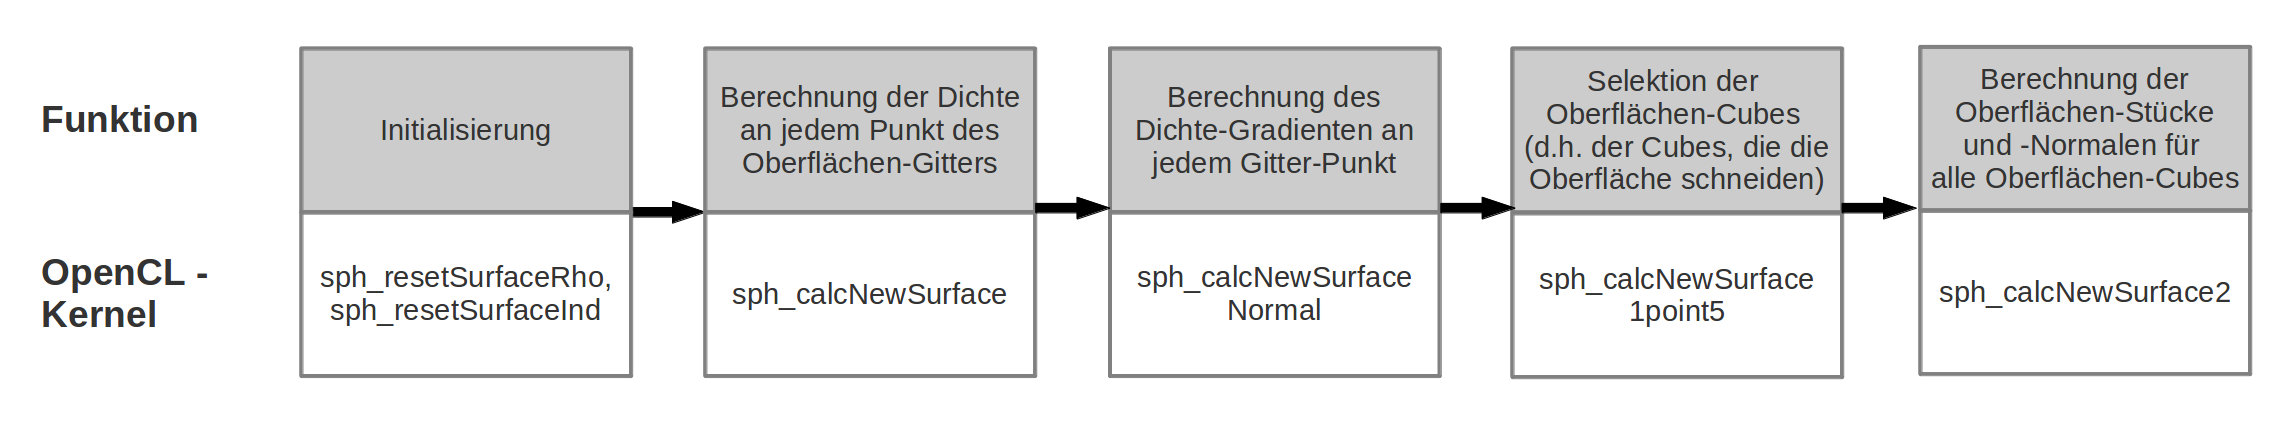
\includegraphics[scale=0.245]{images/MC-Ablauf}
\medskip

\subsubsection*{Berechnung der Gitter-Punkt-Dichten}
Nach der Initialisierung einiger OpenCL-Buffer wird im Kernel {\tt sph\_calcNewSurface} die Dichte an jedem Punkt des Oberflächen-Gitters approximiert. Hierzu wird für jeden Gitter-Punkt $x$ die Dichte $\rho_x$ mittels Gleichung \ref{density} berechnet, also
\begin{align*}
\rho_x = \sum_{i=1}^n m w(x - r_i, h).
\end{align*}
Der naive Ansatz wäre nun, dass je Work-Item sequentiell die obige Summe für einen Gitter-Punkt $x$ berechnet wird. Dies führt allerdings dazu, dass viele Work-Items nichts zu tun haben -- nämlich immer dann, wenn sich der zugehörige Gitter-Punkt außerhalb der Flüssigkeit befindet. Um die Parallelität zu erhöhen hat es sich daher als sinnvoll herausgestellt, für jeden Flüssigkeits-Partikel $i$ ein Work-Item zu starten. In einem OpenCL-Buffer sollen nun für jeden Gitter-Punkt $x$ die Dichten $\rho_x$ abgelegt werden. Hierzu bildet jedes Work-Item die Summanden $m w(x-r_i, h)$ der obigen Dichte-Summe für alle benachbarten Gitter-Punkte $x$ und addiert jeden dieser Summanden mittels der {\tt atomic\_add}-Funktion an die zu $x$ gehörende Stelle des Dichte-Buffers. Es sei noch angemerkt, dass hierbei die Summanden zunächst geeignet skaliert werden, da die {\tt atomic\_add}-Funktion nur Integer-Werte addieren kann.
\medskip
\pagebreak

\subsubsection*{Berechnung der Dichte-Gradienten}
Die Berechnung der Dichte-Gradienten im OpenCL-Kernel {\tt sph\_calcNewSurfaceNormal} erfolgt nach der in \cite[S. 165]{MC} beschriebenen Methode. Jedes Work-Item ist hierbei für die Berechnung des Gradienten an einem der Gitter-Punkte zuständig.
\medskip

\subsubsection*{Selektion der Oberflächen-Cubes}
Nachdem Dichte und Gradienten an den Gitter-Punkten berechnet wurden, kann prinzipiell die Berechnung der Oberflächen-Stücke für jeden Cube des Gitters durchgeführt werden. Hierzu soll sinnvollerweise in einem OpenCL-Kernel für jeden Cube ein Work-Item gestartet werden. Allerdings ist für diejenigen Cubes, die entweder ganz innerhalb oder ganz außerhalb der Flüssigkeit liegen, keine Oberfläche zu berechnen. Bevor daher mit der eigentlichen Oberflächen-Berechnung begonnen wird, werden die Cubes, die tatsächlich von der Oberfläche geschnitten werden, zunächst selektiert. Hierzu wird im Kernel {\tt sph\_calcNewSurface1point5} für jeden Cube des Gittes ein Work-Item gestartet. Jedes Work-Item überprüft nun, ob entweder alle Ecken des Cubes in der Flüssigkeit liegen (d.h. die Dichte an allen Ecken ist größer als ein vorgegebener Schwellenwert) oder ob alle Ecken außerhalb der Flüssigkeit liegen. Tritt einer der beiden Fälle ein, so wird in einem OpenCL-Buffer an der zum betrachteten Cube gehörenden Stelle eine $1$ eingetragen, anderenfalls eine $0$. Anschließend wird dieser Buffer Host-seitig verarbeitet und die Indizes der $0$-Einträge an den Kernel {\tt sph\_calcNewSurface2} übergeben, der für die eigentliche Oberflächen-Berechnung zuständig ist.
\medskip

\subsubsection*{Berechnung der Oberflächen-Stücke und -Normalen}
Zur Berechnung der Oberfläche wird im OpenCL-Kernel {\tt sph\_calcNewSurface2} für jeden zuvor selektierten Oberflächen-Cube ein Work-Item gestartet. Um den Ablauf der Berechnung des Oberflächen-Stückes eines Cubes zu beschreiben, werden zunächst einige Vorbemerkungen benötigt.
\smallskip

\noindent Da jede der acht Ecken eines Cubes entweder in der Flüssigkeit liegt (d.h. die Dichte an diesem Gitter-Punkt übersteigt den Schwellenwert) oder außerhalb, sind zur Bestimmung der richtigen Konfiguration grundsätzlich $2^8 = 256$ Fälle zu unterscheiden. Nummeriert man nun die Ecken mit $1$ bis $8$, so ergibt sich für jeden dieser Fälle ein eindeutiger $8$-Bit-Code, indem das $i$-te Bit genau dann gesetzt wird, wenn die $i$-te Ecke in der Flüssigkeit liegt (vgl. \cite[S. 165]{MC}).
\smallskip

\noindent Mittels diverser Symmetrien (Rotation etc., siehe \cite{MC} und \cite{MCADD} für Details) lassen sich nun die ursprünglichen $256$ Fälle auf einige wenige unterschiedliche Konfigurationen zurückführen. In diesem Projekt werden die Konfigurationen $0$ bis $14$ aus \cite[S. 165]{MC} und zur Vermeidung von Lücken in der Oberfläche ergänzend die Konfigurationen $3a$, $6a$ und $7a$ aus \cite[S. 247]{MCADD} verwendet (letztere erhalten hier die Konfigurations-Nummern $15, 16$ und $17$).
\smallskip
\pagebreak

\noindent Die Zuordnung des 8-Bit-Codes zu einem der insgesamt $18$ unterschiedlichen Konfigurationen wird vor der Simulation in der Java-Klasse {\tt caseMapCreator} berechnet und anschließend in einem constant-Array in den OpenCL-Code geschrieben, welches mit {\tt case\_map} bezeichnet wird. In diesem Array wird für jeden Code zusätzlich zur richtigen Konfigurations-Nummer auch die Permutation der Cube-Ecken abgelegt, die die Ecken der zugeordneten Konfiguration auf die zugehörigen Ecken des ursprünglichen Cubes abbildet.
\smallskip

\noindent Zum Rendern der die Oberfläche darstellenden Dreiecke wird an OpenGL ein Vertex-Buffer und ein Index-Buffer übergeben. Der Vertex-Buffer enthält für jeden Eckpunkt der Oberflächen-Dreiecke sechs Einträge -- die ersten drei geben die räumliche Position des Eckpunktes an und die nächsten drei geben die Oberflächen-Normale an diesem Punkt an. Der Index-Buffer enthält für jedes Oberflächen-Dreieck drei aufeinander folgende Indizes, die sich auf den Vertex-Buffer beziehen und die Eckpunkte des zu zeichnenden Dreiecks festlegen.
\smallskip


\noindent Betrachtet man nun das Oberflächen-Stück eines Oberflächen- Cubes, so liegen die Eckpunkte der Dreiecke, die dieses Stück definieren, genau auf denjenigen Kanten des Cubes, deren eine Ecke innerhalb und deren andere Ecke außerhalb der Flüssigkeit liegt (vgl. \cite[S. 164]{MC}). Jede der $18$ Konfigurationen ist daher genau festgelegt durch die Angabe der beteiligten Kanten für die Eckpunkte und eine Angabe von Indizes, durch die bestimmt ist, welche der Eckpunkte die Dreiecke bilden. Hierzu werden die Kanten des Cubes von $1$ bis $12$ nummeriert. Wie schon die Nummerierung der Ecken folgt auch die in diesem Projekt verwendete Nummerierung der Kanten dem Vorschlag in \cite[S. 165]{MC}. Die Angabe der beteiligten Kanten für jede Konfiguration sowie die Angabe der die Dreiecke definierenden Indizes wird nun in zwei separaten constant-Arrays abgelegt, die mit {\tt confVertex} und {\tt confIndex} bezeichnet werden.
\smallskip


\noindent Wenn nun für einen konkreten Oberflächen-Cube das Oberflächen-Stück berechnet werden soll, so wird zunächst der $8$-Bit-Code berechnet und mittels des {\tt case\_map}-Arrays die richtige Konfigurations-
Nummer bestimmt. Mithilfe dieser Nummer lassen sich aus dem {\tt confIndex}-Array die richtigen Indizes für den OpenGL-Index-Buffer auslesen. Um die richtigen Werte für den OpenGL-Vertex-Buffer zu erhalten, müssen zunächst für jede im {\tt confVertex}-Array hinterlegte Kanten-Nummer die räumliche Position des zugehörigen Dreiecks-Eckpunktes und die Oberflächen-Normale an dieser Stelle berechnet werden. Für jede Kanten-Nummer werden hierzu aus dem constant-Array {\tt edgesToVerts} die zwei zugehörigen Ecken-Nummern ausgelesen. Die Ecken-Nummern werden dann mittels der im {\tt case\_map}-Array hinterlegten Permutation auf die entsprechenden Ecken im ursprünglichen Cube abgebildet. Interpoliert man nun diese ursprünglichen Cube-Ecken mittels der Dichte-Werte an diesen Gitter-Punkten, so erhält man die gewünschte Position des Dreiecks-Eckpunktes und eine analoge Interpolation der zugehörigen Dichte-Gradienten liefert zudem die Normale (vgl. \cite[S. 165]{MC}).
\smallskip

\noindent Abschließend illustriert das folgende Schaubild noch einmal anhand eines Beispiels den Ablauf der Berechnung eines Oberflächen-Stückes. Wie auch bei den Zeichnungen in \cite[S. 165]{MC} werden dabei die in der Flüssigkeit liegenden Cube-Ecken mit schwarzen Punkten gekennzeichnet. Es sei noch angemerkt, dass für die Nummerierung der Cube-Ecken an einigen Stellen die Zahlen $0$ bis $7$ anstatt $1$ bis $8$ verwendet werden.
\medskip

\begin{center}
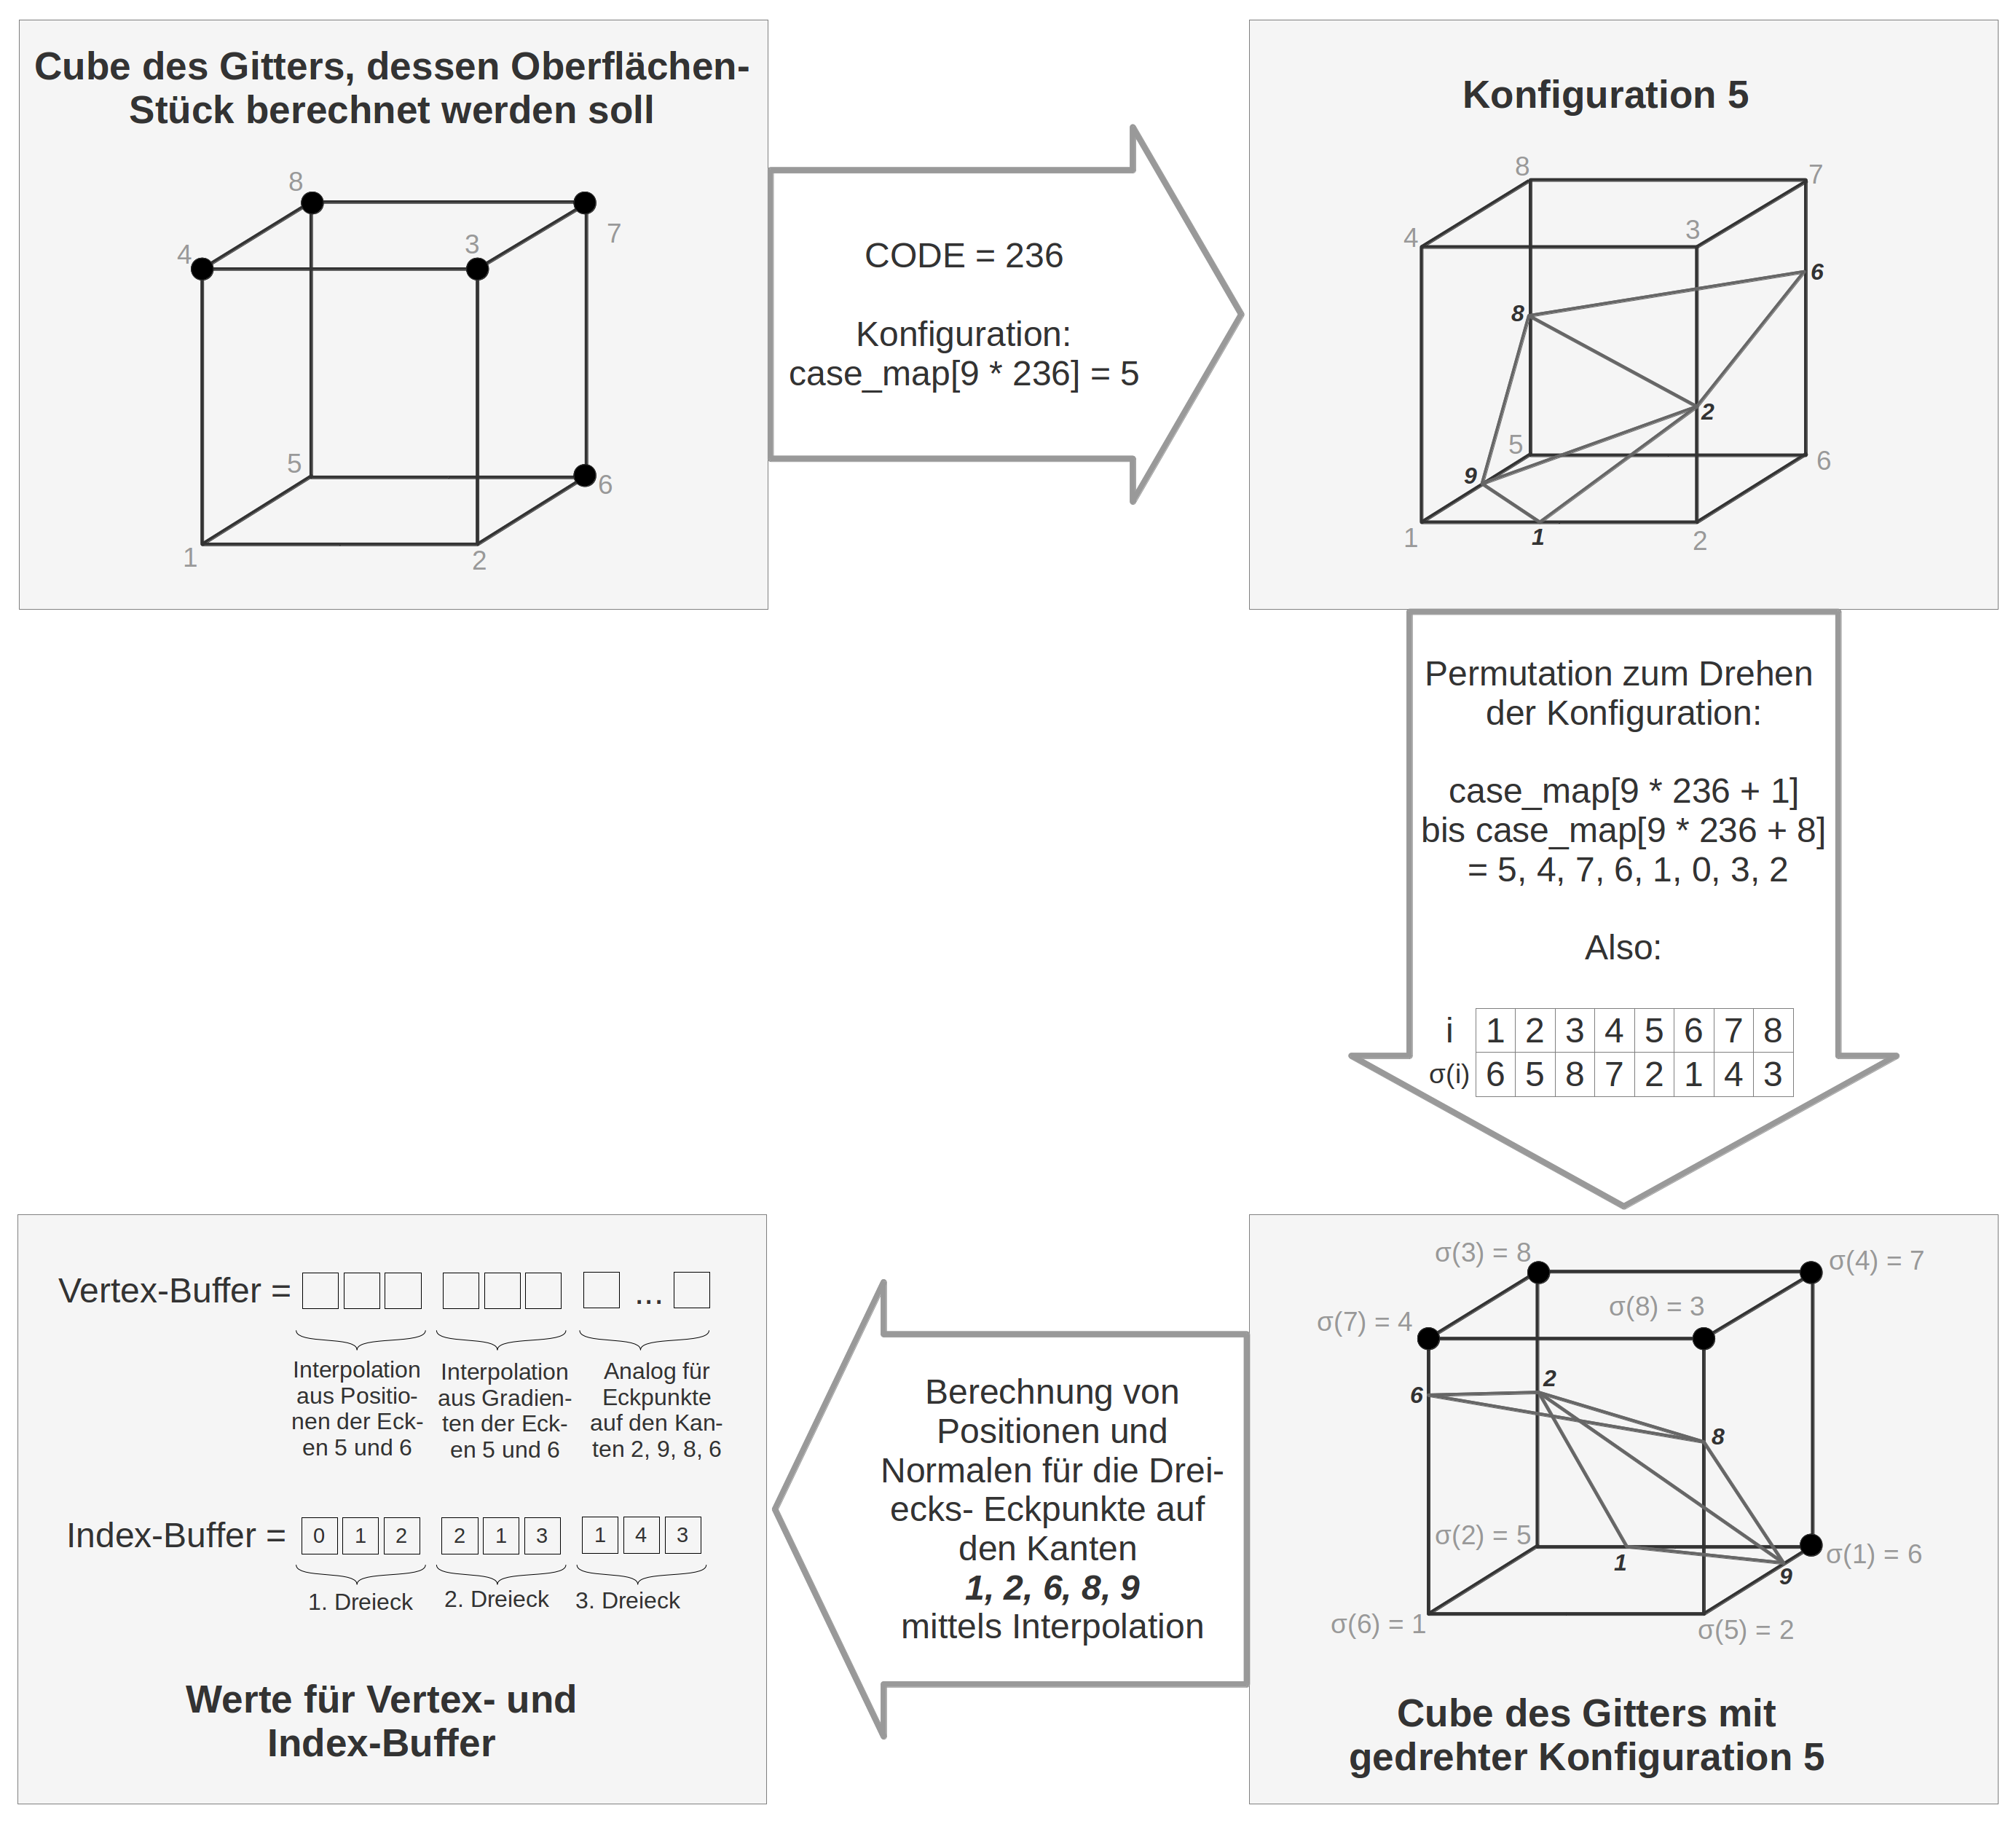
\includegraphics[scale=0.2]{images/Cube-Ablauf}
\end{center}
\newpage
\pagebreak
\section{Deferred Shading}

\begin{center}
\emph{{\small Tobias Graf}}
\end{center}

\bigskip

\subsubsection*{Einleitung} Um aus der entstandenen Drahtgitter - Oberfläche des Marching Cubes Algorithmus eine Näherung zu einer Wasseroberfläche zu erzielen verwenden wir Deferred Shading. In diesem Kapitel wird kurz erläutert was Deferred Shading generell ist und wie unsere Implementierung das ganze Nutzt um einen Transparenten Wassereffekt zu erreichen.

\subsection*{Deferred Shading} Ursprünglich ist Deferred Shading eine Technik der Computergrafik um die Lichtberechnung von der Geometrieberechnung zu trennen. Sie erlaubt durch das Reduzieren der Komplexität wesentlich mehr Lichtobjekte in einer Szene als bei klassischen Rendermethoden, in denen anhand der Tiefe, Normale und Farbwert eines Eckpunktes in Korrelation einer Lichtquelle die Dargestellte Farbe berechnet wurden. Beim Deferred Shading werden durch sogenannte Framebufferobjekte (FBO) Tiefenwerte, Normale und Farbe der Geometrien in eine Textur mit Bildschirmauflösung gerendert. Statt nun für jeden Geometrischen Eckpunkt den Farbwert zu berechnen wird dies nun für jeden Pixel angewandt wodurch der Aufwand von $O(m*n)$ auf $O(m+n)$ reduziert wird. Nachteilig dabei ist das zwar weniger Hardwareanforderungen benötigt werden um die gleiche Szene zu rendern, jedoch der Speicherverbrauch extrem ansteigt da die Texturen im Grafikkartenspeicher vorgehalten werden müssen.\\
Relativ schnell Entwickelten sich vielfältige Nutzungen der Technik zur Berechnung von Shadow Maps und einsetzen von Postprocessing Effekten.

\subsection*{Unser Ansatz} Angelehnt an den Ansatz des GDC Vortrags\cite{DSGDC} erfolgte zuerst die Implementation mehrerer Framebufferobjekte die als einzelne Rendertargets benutzt werden um verschiedene Aspekte der Szene einzeln in Texturen zu Rendern. Die Aufteilung erfolgt in folgende FBO und Grafiken:
\begin{itemize}
\item Hintergrund
\item Thickness
\item Partikel
	\begin{itemize}
	\item Farbwert
	\item Tiefenwert
	\item Welt - Koordinate
	\item Normale
	\item Spekulare Farbe
	\item Diffuse Farbe
	\end{itemize}
\end{itemize}  
\medskip
\noindent Das getrennte Rendern des Hintergrundes ist notwendig um den Transparenz Effekt zu erreichen da dies eine schwäche von Deferred Shading ist da man keinen nutzen aus der \texttt{GL_BLEND} Funktion ziehen kann wenn die einzelnen Geometrien in getrennten FBO gezeichnet werden. Die Thickness bestimmt im abschließenden Bild die Hauptsächliche Transparenz der Oberfläche. Der Partikel FBO schreibt die einzelnen Parameter mit denen die Lichtberechnung des Phong Modells und die Farbgebung des Objektes in die jeweiligen Texturen.
\begin{align*}
\noindent
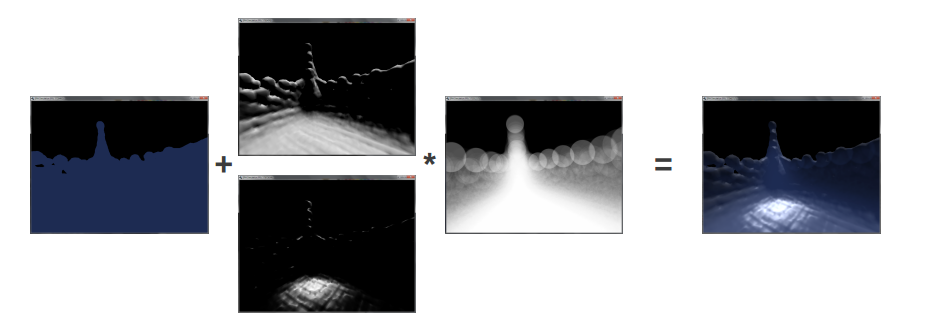
\includegraphics[scale=0.9]{images/Dereffered}
\end{align*}
\medskip  


\begin{thebibliography}{}


\bibitem{IntroSPH}
J.\ J.\ Monaghan (1988),
{\em An Introduction to SPH}. Computer Physics Communication, Vol. 48, pp. 89-96.


\bibitem{FlowSPH}
J.\ J.\ Monaghan (1994),
{\em Simulating Free Surface Flows with SPH}. Journal of Computational Physics, Vol. 110, pp. 399-406.


\bibitem{FluidSim}
M.\ Müller, D.\ Charypar, M.\ Gross (2003),
{\em Particle-Based Fluid Simulation for Interactive Applications}. Proceedings of the 2003 ACM SIGGRAPH/Eurographics symposium on Computer animation, pp. 154-159.


\bibitem{BoundarySPH}
T.\ Harada, S.\ Koshizuka and Y.\ Kawaguchi (2007),
{\em Improvement in the Boundary Conditions of Smoothed Particle Hydrodynamics}. Computer Graphics \& Geometry, Vol. 9, No. 3, pp. 2-15.


\bibitem{MC}
W.\ E.\ Lorensen, H.\ E.\ Cline (1987),
{\em Marching cubes: A high resolution 3D surface construction algorithm}. SIGGRAPH Comput. Graph., Vol. 21, No. 4, pp. 163-169.


\bibitem{MCADD}
W.\ Heiden, T.\ Goetze, J.\ Brickmann (1993). {\em Fast generation of molecular surfaces from 3D data fields with an enhanced ``marching cube'' algorithm}. Journal of Computational Chemistry, Vol. 14, Iss. 2, pp. 246-250.

\end{thebibliography}


\end{document}